% Manual de Arturito R2D2 — robot recolector de limones (Grupo 2, FIUNA Mecatrónica, 2026S2)
% Compilar desde docs/manual:  pdflatex manual && pdflatex manual   (dos pasadas: índice y referencias)
% Las figuras de los HTML se regeneran con:  python3 capturar.py
\documentclass[11pt,a4paper,oneside]{report}

\usepackage[T1]{fontenc}
\usepackage[utf8]{inputenc}
\DeclareUnicodeCharacter{2212}{\ensuremath{-}}
\DeclareUnicodeCharacter{2192}{\ensuremath{\rightarrow}}
\DeclareUnicodeCharacter{2190}{\ensuremath{\leftarrow}}
\DeclareUnicodeCharacter{2265}{\ensuremath{\geq}}
\DeclareUnicodeCharacter{2264}{\ensuremath{\leq}}
\DeclareUnicodeCharacter{2248}{\ensuremath{\approx}}
\DeclareUnicodeCharacter{03A9}{\ensuremath{\Omega}}
\DeclareUnicodeCharacter{0394}{\ensuremath{\Delta}}
\DeclareUnicodeCharacter{03B3}{\ensuremath{\gamma}}
\DeclareUnicodeCharacter{03BC}{\ensuremath{\mu}}
\DeclareUnicodeCharacter{03B8}{\ensuremath{\theta}}
\DeclareUnicodeCharacter{03C9}{\ensuremath{\omega}}
\DeclareUnicodeCharacter{2026}{\ldots}
\usepackage[spanish,es-noshorthands,es-tabla]{babel}
\usepackage{lmodern}
\usepackage{microtype}
\usepackage[a4paper,margin=2.3cm,headheight=14pt]{geometry}
\usepackage{amsmath,amssymb,mathtools}
\usepackage{icomma}
\usepackage[table]{xcolor}
\usepackage{graphicx}
\usepackage{float}
\usepackage{caption}
\usepackage{subcaption}
\usepackage{booktabs,tabularx,longtable,multirow,makecell}
\usepackage{enumitem}
\usepackage{fancyhdr}
\usepackage{titlesec}
\usepackage{pifont}
\usepackage{listings}
\usepackage[most]{tcolorbox}
\usepackage{tikz}
\usetikzlibrary{positioning,arrows.meta,shapes.geometric,shapes.misc,fit,calc,backgrounds,decorations.pathreplacing,matrix}
\usepackage[hidelinks]{hyperref}

% ---------------------------------------------------------------- colores
\definecolor{tinta}{HTML}{17231F}
\definecolor{gris}{HTML}{56655F}
\definecolor{suave}{HTML}{E4EBE7}
\definecolor{acento}{HTML}{2A66AD}
\definecolor{verde}{HTML}{237A4F}
\definecolor{rojo}{HTML}{C2362C}
\definecolor{naranja}{HTML}{CF7A12}
\definecolor{violeta}{HTML}{8646B8}
\definecolor{ocre}{HTML}{A8740A}
\definecolor{fondocod}{HTML}{F4F6F5}

% ---------------------------------------------------------------- títulos y encabezados
\titleformat{\chapter}[display]{\normalfont\bfseries\color{tinta}}
  {\color{acento}\large\MakeUppercase{Capítulo}~\thechapter}{6pt}{\Huge}
\titlespacing*{\chapter}{0pt}{-10pt}{24pt}
\titleformat{\section}{\normalfont\Large\bfseries\color{tinta}}{\color{acento}\thesection}{0.8em}{}
\titleformat{\subsection}{\normalfont\large\bfseries\color{tinta}}{\color{acento}\thesubsection}{0.8em}{}
\pagestyle{fancy}
\fancyhf{}
\fancyhead[L]{\small\color{gris}Arturito R2D2 · Manual del sistema}
\fancyhead[R]{\small\color{gris}\nouppercase{\leftmark}}
\fancyfoot[C]{\small\thepage}
\renewcommand{\headrulewidth}{0.4pt}
\setlength{\parindent}{0pt}
\setlength{\parskip}{6pt}
\setlength{\emergencystretch}{3em}
\setlist{itemsep=2pt,topsep=4pt}
\captionsetup{font=small,labelfont=bf}

% ---------------------------------------------------------------- código
\lstdefinestyle{base}{
  basicstyle=\ttfamily\footnotesize, backgroundcolor=\color{fondocod}, frame=single, rulecolor=\color{suave},
  breaklines=true, breakatwhitespace=false, columns=fullflexible, keepspaces=true, showstringspaces=false,
  commentstyle=\color{gris}\itshape, keywordstyle=\color{acento}\bfseries, stringstyle=\color{verde},
  xleftmargin=4pt, xrightmargin=4pt, aboveskip=6pt, belowskip=6pt,
  literate={á}{{\'a}}1 {é}{{\'e}}1 {í}{{\'i}}1 {ó}{{\'o}}1 {ú}{{\'u}}1 {ñ}{{\~n}}1 {Á}{{\'A}}1 {É}{{\'E}}1
           {Í}{{\'I}}1 {Ó}{{\'O}}1 {Ú}{{\'U}}1 {Ñ}{{\~N}}1 {°}{{\textdegree}}1 {¿}{{?`}}1 {¡}{{!`}}1
           {→}{{$\rightarrow$}}2 {←}{{$\leftarrow$}}2 {·}{{$\cdot$}}1 {≥}{{$\geq$}}1 {≤}{{$\leq$}}1 {×}{{$\times$}}1
           {µ}{{$\mu$}}1 {²}{{$^2$}}1 {±}{{$\pm$}}1 {−}{{-}}1 {…}{{...}}3 {Ω}{{$\Omega$}}1 {—}{{---}}1 {–}{{--}}1 {ü}{{\"u}}1 {“}{{``}}1 {”}{{''}}1 {Δ}{{$\Delta$}}1 {≈}{{$\approx$}}1 {✓}{{v}}1
}
\lstset{style=base}
\lstdefinelanguage{consola}{morekeywords={ros2,colcon,source,pio,ssh,cd,export,sudo,python3,rsync,git},sensitive=true,
  morecomment=[l]\#}

% ---------------------------------------------------------------- cajas
\newtcolorbox{nota}[1][Nota]{colback=acento!5,colframe=acento,fonttitle=\bfseries,title={#1},boxrule=0.6pt,arc=2pt,left=6pt,right=6pt}
\newtcolorbox{peligro}[1][Cuidado]{colback=rojo!5,colframe=rojo,fonttitle=\bfseries,title={#1},boxrule=0.6pt,arc=2pt,left=6pt,right=6pt}
\newtcolorbox{idea}[1][En pocas palabras]{colback=verde!6,colframe=verde,fonttitle=\bfseries,title={#1},boxrule=0.6pt,arc=2pt,left=6pt,right=6pt}
\newtcolorbox{pendiente}[1][Pendiente de medir o probar]{colback=naranja!6,colframe=naranja,fonttitle=\bfseries,title={#1},boxrule=0.6pt,arc=2pt,left=6pt,right=6pt}

% ---------------------------------------------------------------- TikZ
\tikzset{
  >={Stealth[length=2.2mm]},
  caja/.style={draw=tinta,rounded corners=2pt,fill=white,align=center,font=\small,minimum height=8mm,inner sep=4pt},
  placa/.style={caja,fill=suave,font=\small\bfseries},
  nodo/.style={draw=acento,fill=acento!8,rounded corners=6pt,align=center,font=\small,minimum height=8mm,inner sep=4pt},
  topico/.style={font=\scriptsize\ttfamily,fill=white,inner sep=1pt},
  estado/.style={draw=tinta,fill=white,rounded corners=8pt,align=center,font=\small\bfseries,minimum height=8mm,minimum width=20mm},
  estadorojo/.style={estado,draw=rojo,fill=rojo!8},
  grupo/.style={draw=gris,dashed,rounded corners=4pt,inner sep=7pt},
  flecha/.style={->,thick,draw=tinta},
  datos/.style={->,thick,draw=acento},
  gpio/.style={->,thick,draw=verde},
  pot/.style={->,very thick,draw=rojo},
  logica/.style={->,very thick,draw=naranja},
  seg/.style={->,thick,draw=violeta},
}

% En \cod, \topic y \archivo se puede cortar la línea después de "_" (rutas y nombres largos)
\usepackage{xstring}
\newcommand{\codus}{\textunderscore\allowbreak}
\newcommand{\cortable}[1]{\let\_\codus\noexpandarg\StrSubstitute{#1}{/}{/\allowbreak}}
\DeclareRobustCommand{\cod}[1]{\leavevmode{\ttfamily\cortable{#1}}}
\DeclareRobustCommand{\topic}[1]{\leavevmode{\ttfamily\color{acento}\cortable{#1}}}
\DeclareRobustCommand{\archivo}[1]{\leavevmode{\ttfamily\color{gris}\cortable{#1}}}
\newcommand{\ok}{\textcolor{verde}{\ding{51}}}
\newcommand{\no}{\textcolor{rojo}{\ding{55}}}

\graphicspath{{figuras/}}

\begin{document}

% ================================================================ portada
\begin{titlepage}
  \thispagestyle{empty}
  \begin{tikzpicture}[remember picture,overlay]
    \fill[tinta] (current page.north west) rectangle ([yshift=-9cm]current page.north east);
    \fill[acento] ([yshift=-9cm]current page.north west) rectangle ([yshift=-9.25cm]current page.north east);
  \end{tikzpicture}
  \vspace*{0.4cm}
  {\color{white}\small\sffamily FACULTAD DE INGENIERÍA · UNIVERSIDAD NACIONAL DE ASUNCIÓN\\
  Ingeniería Mecatrónica · Robótica I y Robótica II · 2026S2\par}
  \vspace{1.6cm}
  {\color{white}\fontsize{34}{40}\selectfont\bfseries Arturito R2D2\par}
  \vspace{0.3cm}
  {\color{white}\Large Robot móvil autónomo recolector de limones\par}
  \vspace{0.2cm}
  {\color{acento!40}\large Manual completo del sistema: hardware, electrónica, firmware, ROS 2, visión y operación\par}
  \vspace{1.4cm}
  \begin{center}
    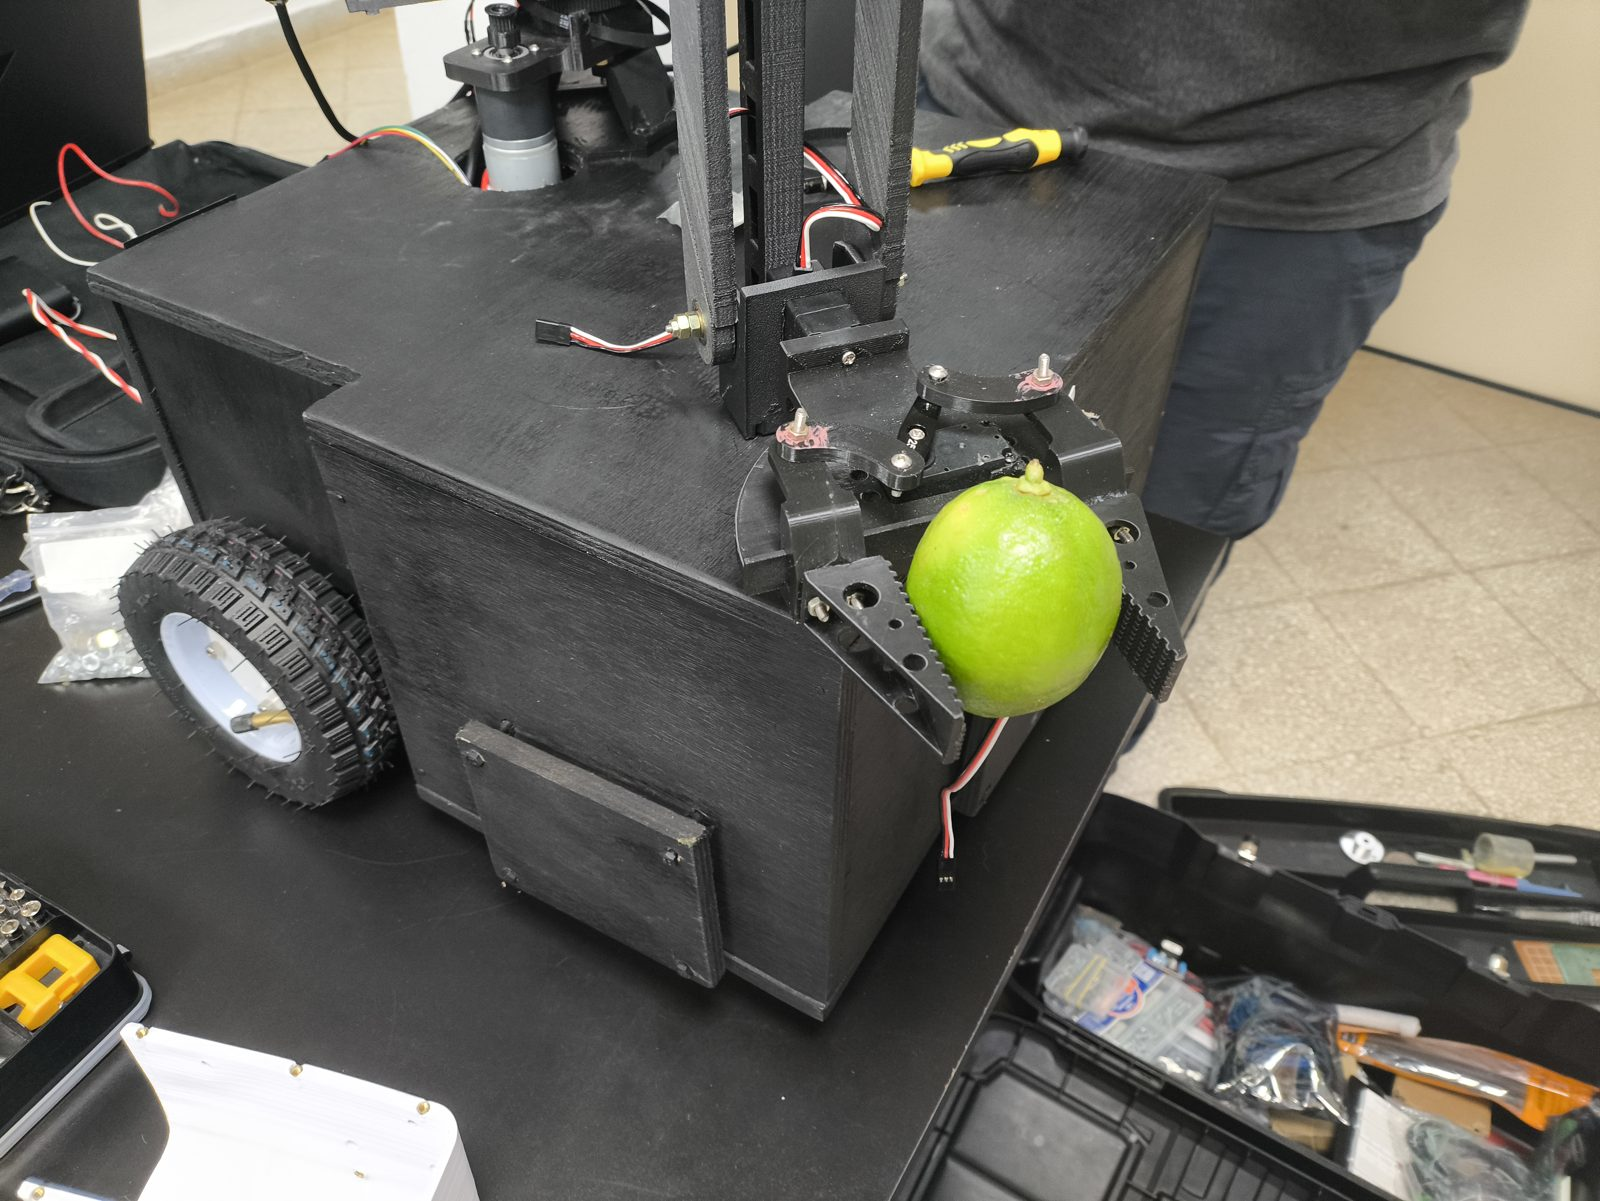
\includegraphics[height=7.2cm]{robot_limon.jpg}\hspace{3mm}%
    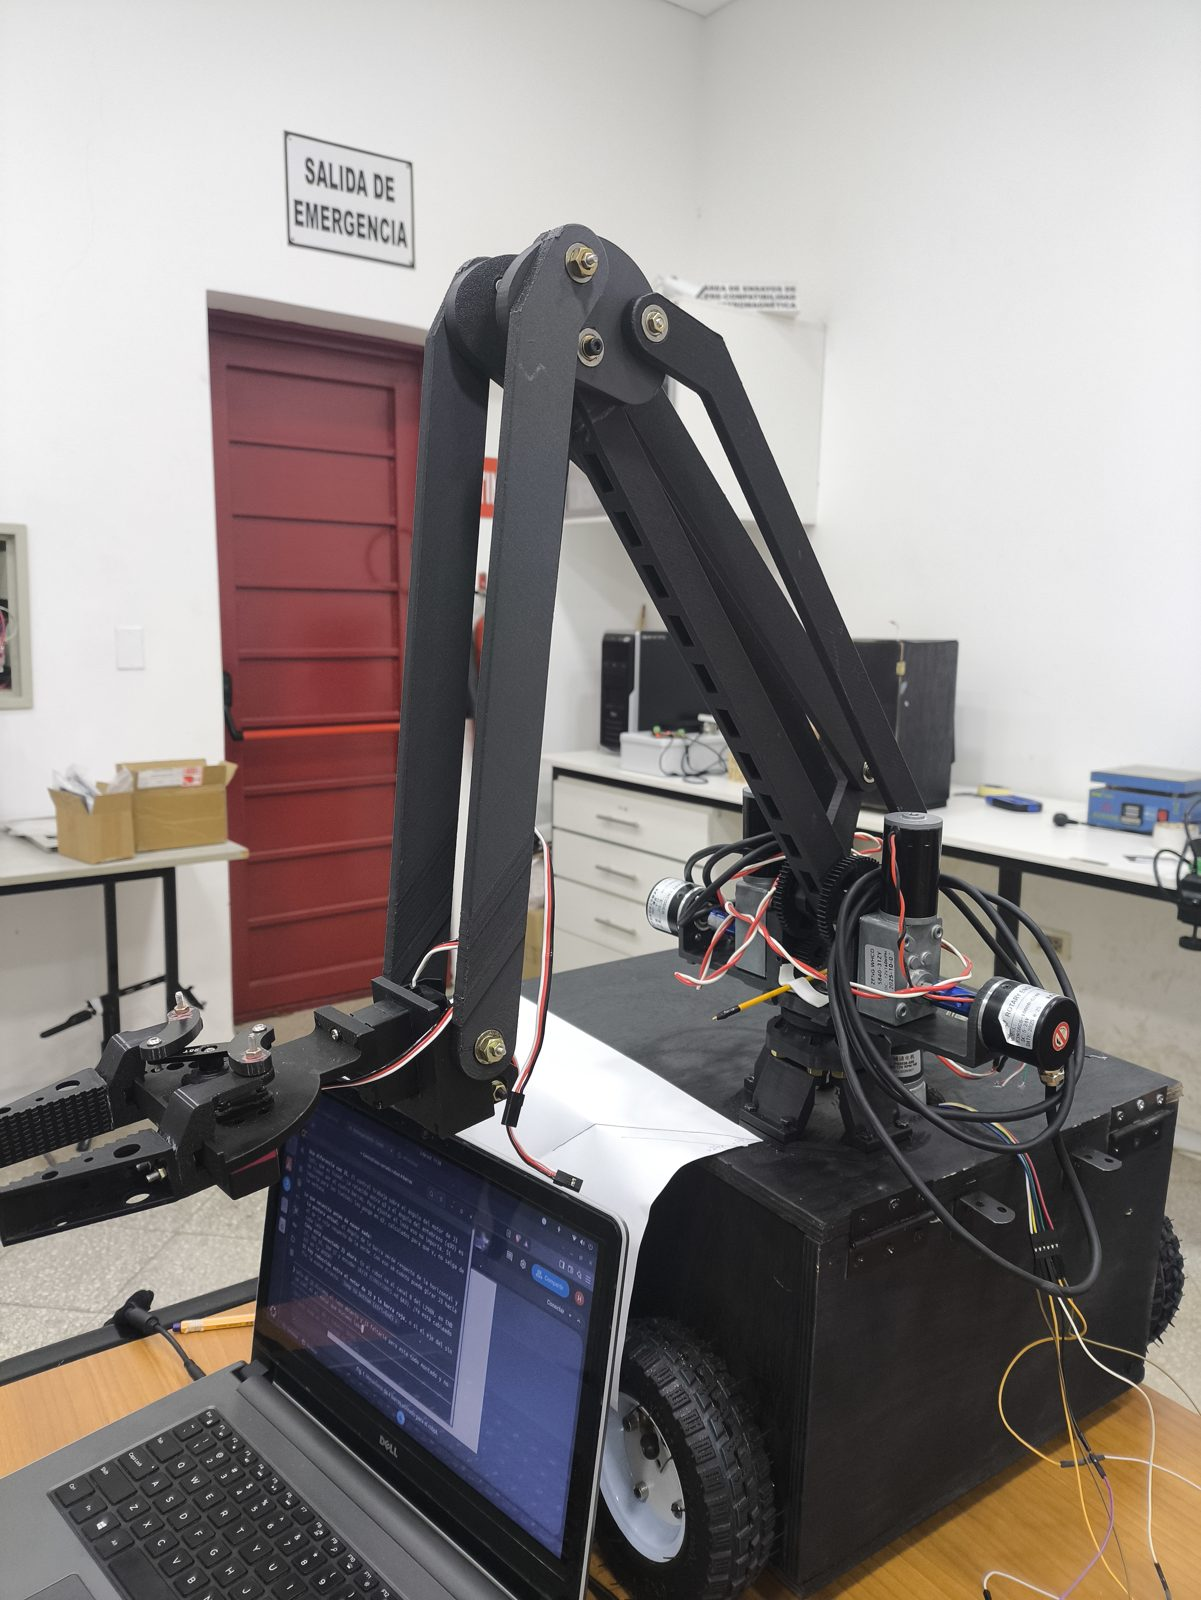
\includegraphics[height=7.2cm]{robot2.jpg}
  \end{center}
  \vfill
  {\large\bfseries Grupo 2\par}
  {\color{gris} Versión 1.0 · 14 de octubre de 2026 · estado del proyecto a esa fecha\par}
  {\color{gris}\small Repositorios: \texttt{HecVelaz/recolector\_de\_frutas} (robot) y \texttt{HecVelaz/vision\_estereo} (visión)\par}
\end{titlepage}

\pagenumbering{roman}
\tableofcontents
\clearpage
\pagenumbering{arabic}

\chapter{Introducción}

\section{Qué es Arturito R2D2}

Arturito R2D2 es un robot móvil que recorre el pasillo entre dos hileras de limoneros, encuentra los limones con
una cámara, calcula dónde están en el espacio y los cosecha con un brazo articulado. Es el trabajo práctico final del
Grupo~2 para dos materias a la vez:

\begin{itemize}
  \item \textbf{Robótica I} evalúa el \textbf{brazo}: un manipulador RRR (tres articulaciones rotativas) tipo
        uArm / Dobot Magician, con una pinza de dos servos.
  \item \textbf{Robótica II} evalúa el \textbf{robot móvil}: la base con tracción diferencial, los sensores, la
        seguridad, la integración con ROS~2 y la autonomía.
\end{itemize}

\begin{idea}[Objetivo mínimo para aprobar]
El robot \textbf{se mueve}, \textbf{detecta el limón con YOLO}, \textbf{lo localiza en 3D con visión estéreo} y
\textbf{lo agarra} con el brazo. Todo lo demás (GPS, app móvil, clasificación por tamaño, 30 frutos medidos) viene
después de que esto funcione de punta a punta.
\end{idea}

El limón no figura entre las especies de la guía de Robótica~II, pero su uso fue aprobado por el profesor. También
se aprobó que la herramienta sea una \textbf{pinza con agarre, tracción y giro} en vez de la ventosa de succión que
proponía la consigna.

\begin{figure}[H]
  \centering
  \begin{subfigure}{0.32\textwidth}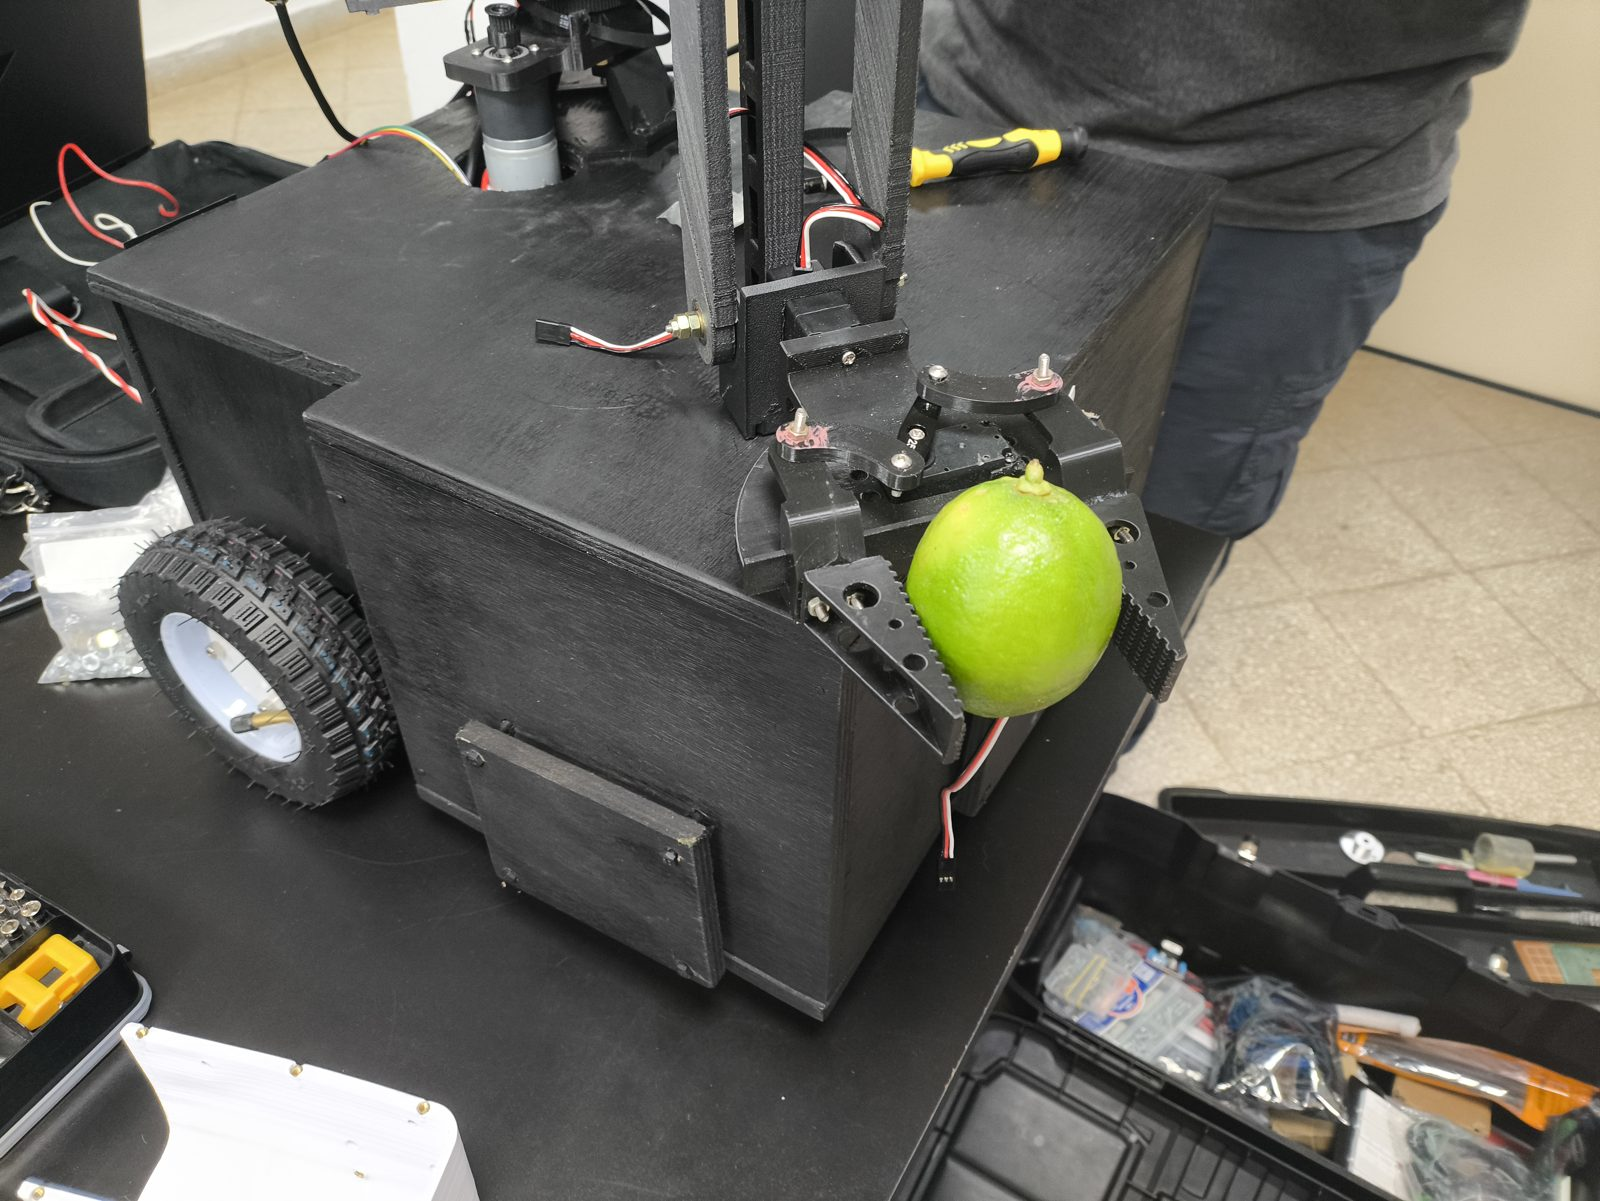
\includegraphics[width=\linewidth]{robot_limon.jpg}\caption{Agarrando un limón.}\end{subfigure}\hfill
  \begin{subfigure}{0.32\textwidth}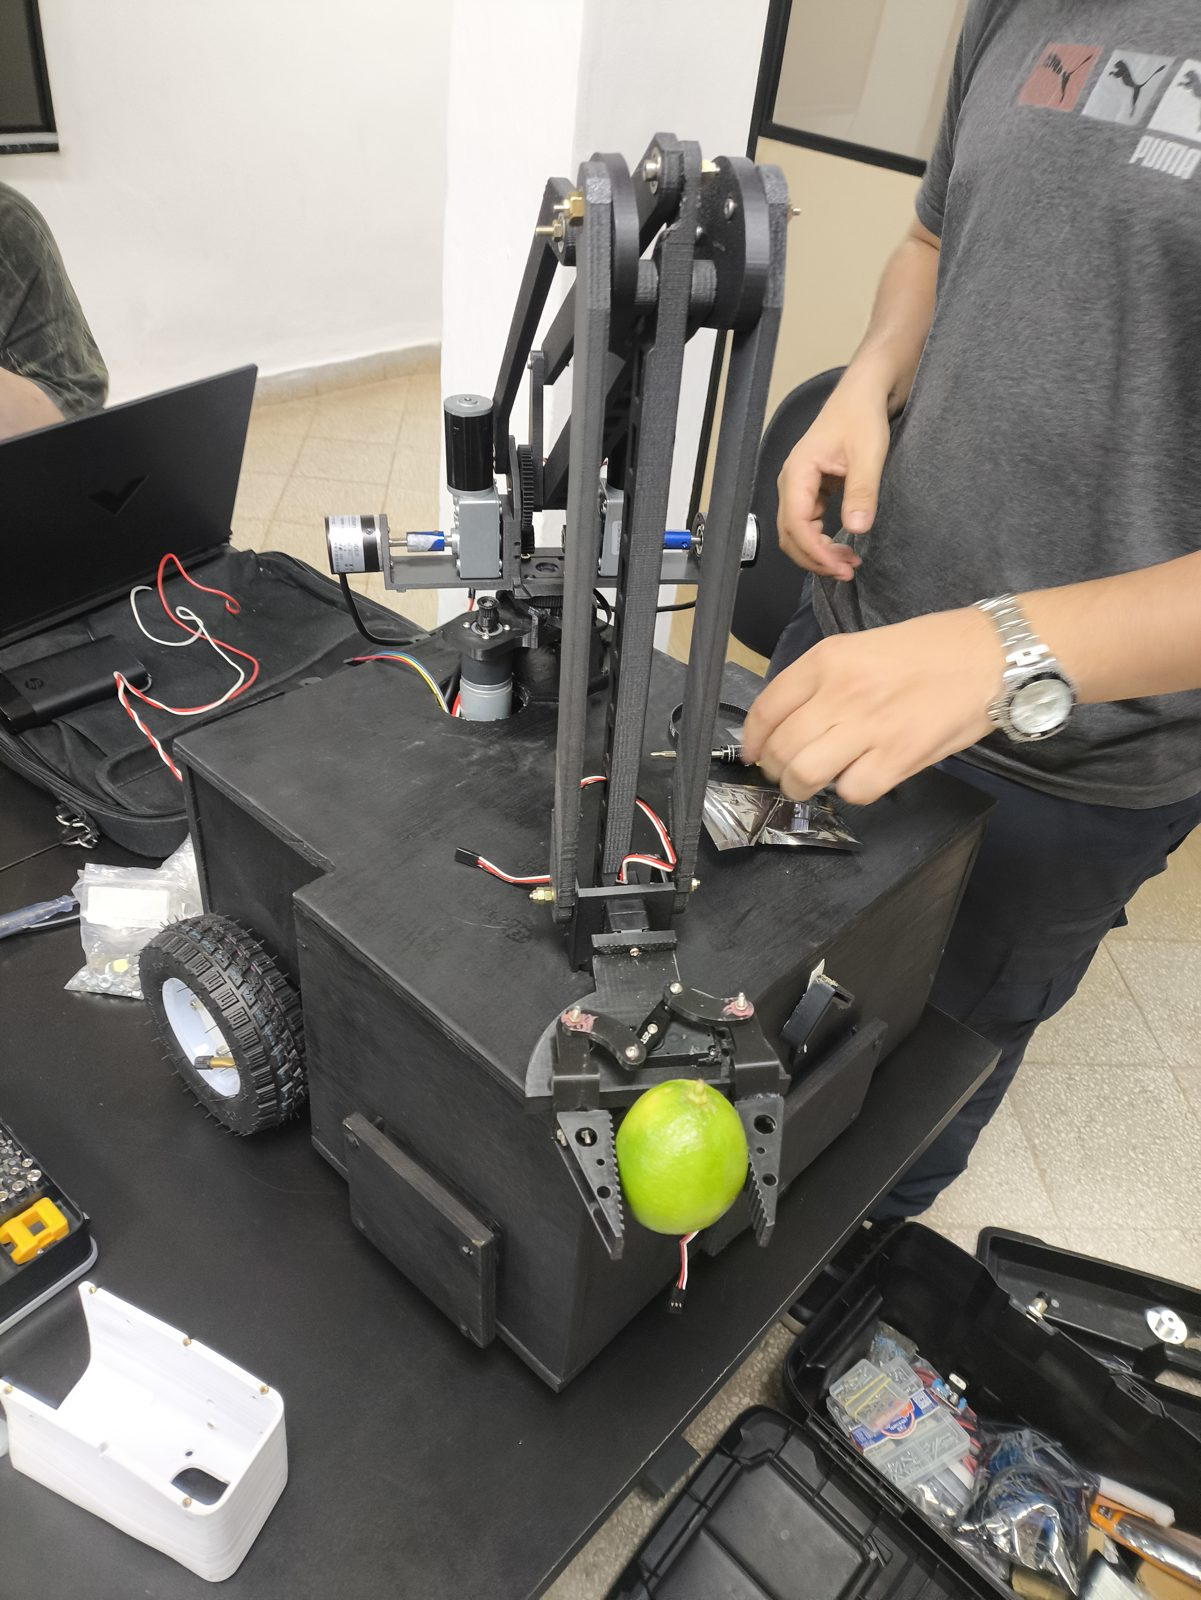
\includegraphics[width=\linewidth]{robot3.jpg}\caption{Brazo sobre la base.}\end{subfigure}\hfill
  \begin{subfigure}{0.32\textwidth}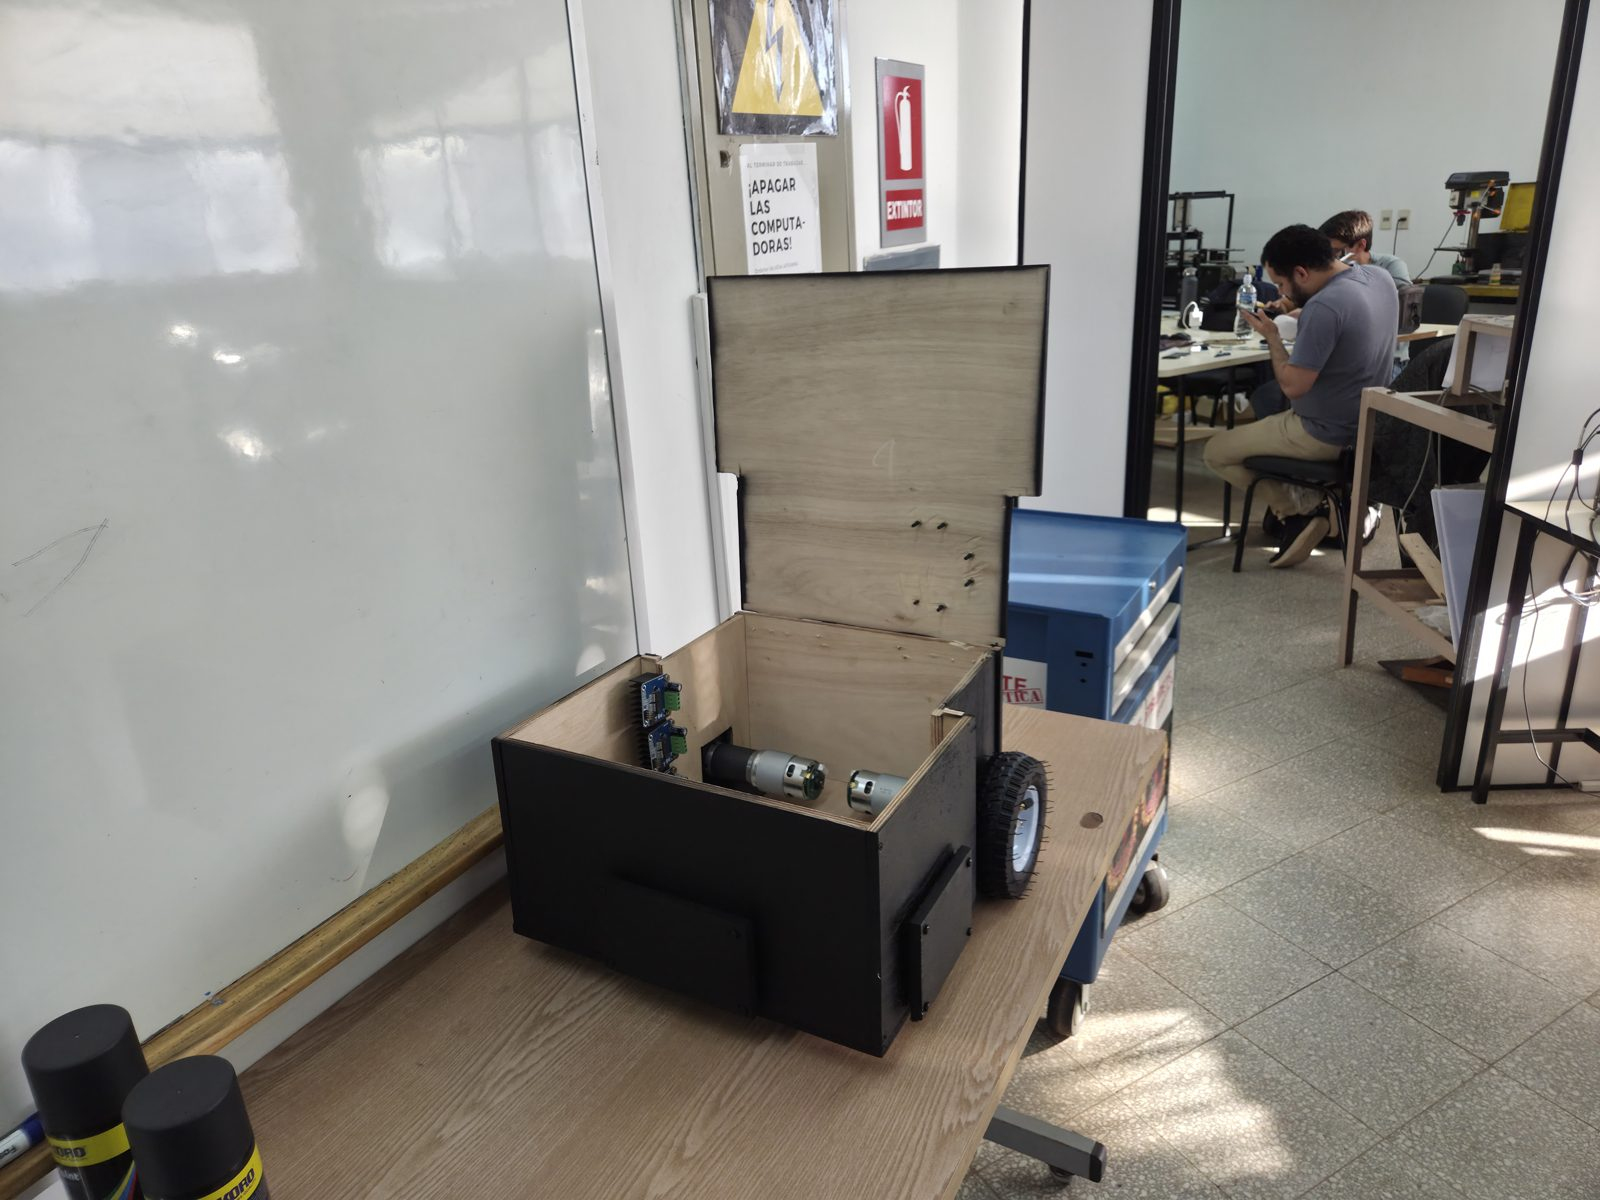
\includegraphics[width=\linewidth]{robot_montado.jpg}\caption{Base de madera en T.}\end{subfigure}
  \caption{El robot en el laboratorio (fotos de las entregas R1~E6 y R2~E3).}
\end{figure}

\section{Cómo leer este manual}

El manual va de lo físico a lo lógico y termina con procedimientos. Se puede leer de corrido o ir directo a lo que
se necesite:

\begin{center}
\begin{tabularx}{\textwidth}{@{}l X@{}}
\toprule
\textbf{Si querés\ldots} & \textbf{Leé} \\
\midrule
Entender el sistema completo en 10 minutos & Capítulo~\ref{cap:general} (vista general) \\
Saber qué es cada pieza física & Capítulos~\ref{cap:mecanica} (mecánica) y \ref{cap:potencia} (potencia) \\
Cablear una placa & Capítulo~\ref{cap:placas} \\
Entender qué hace el código de los ESP32 & Capítulo~\ref{cap:firmware} \\
Aprender ROS~2 desde cero (publicar, suscribir, \textit{launch}) & Capítulo~\ref{cap:ros2} \\
Entender el ``armar'' y cómo hablan la Pi y los ESP32 & Capítulo~\ref{cap:microros} \\
Entender cómo se encuentra el limón en 3D & Capítulo~\ref{cap:vision} \\
Entender cómo se calculan los ángulos del brazo & Capítulo~\ref{cap:ik} \\
Entender cómo decide el robot cuándo frenar y cuánto avanzar & Capítulo~\ref{cap:mision} \\
Probar todo sin hardware & Capítulo~\ref{cap:sim} (Gazebo) \\
Encender el robot por primera vez, paso a paso & Capítulo~\ref{cap:marcha} \\
Arreglar algo que no anda & Capítulo~\ref{cap:diag} \\
Saber qué falta & Capítulo~\ref{cap:estado} \\
Buscar un tópico, un comando o un parámetro & Apéndice~\ref{ap:ref} \\
\bottomrule
\end{tabularx}
\end{center}

\subsection*{Convenciones}
\begin{itemize}
  \item \topic{/cmd\_vel}: un \textbf{tópico} de ROS~2 (un ``canal'' de mensajes).
  \item \archivo{firmware/base/include/pins.h}: un \textbf{archivo} del repositorio \cod{recolector\_de\_frutas}.
  \item \cod{armar}: un \textbf{comando} o texto que se escribe tal cual.
  \item Unidades del Sistema Internacional en todo ROS~2: metros, radianes, segundos. El firmware del brazo trabaja
        internamente en grados y la capa micro-ROS convierte.
  \item Los valores marcados \textbf{MEDIR} son estimaciones: hay que reemplazarlos por lo medido en el robot real.
\end{itemize}

\begin{nota}[Cajas de este manual]
Las cajas azules son notas; las verdes, resúmenes; las rojas, \textbf{cosas que pueden romper algo o lastimar}; las
naranjas, valores o pruebas que todavía faltan.
\end{nota}

\section{Glosario rápido}

\begin{longtable}{@{}p{3.2cm} p{12.3cm}@{}}
\toprule
\textbf{Término} & \textbf{Qué significa acá} \\
\midrule
\endhead
ROS~2 (Jazzy) & \textit{Robot Operating System}: no es un sistema operativo sino un conjunto de bibliotecas y
  herramientas para que muchos programas (nodos) intercambien mensajes. Corre en la Raspberry Pi. \\
Nodo & Un programa de ROS~2. Ej.: el detector YOLO, la cinemática inversa, la misión. \\
Tópico & Canal con nombre por donde viajan mensajes de un tipo fijo. Ej.: \topic{/cmd\_vel} lleva
  \cod{geometry\_msgs/Twist}. \\
Publicar / suscribir & Mandar mensajes a un tópico / recibirlos. Cualquiera puede publicar o suscribirse. \\
micro-ROS & ROS~2 reducido que corre en un microcontrolador (los ESP32). Necesita un \textbf{agente} en la Pi
  que lo conecte con el resto. \\
Agente micro-ROS & Programa en la Pi que hace de puente entre el ESP32 (por USB serie) y la red de ROS~2. \\
Armar / desarmar & Seguro por sesión de cada ESP32: desarmado no acepta órdenes de movimiento
  (capítulo~\ref{cap:microros}). \\
ESP32-S3 & Microcontrolador de la \textbf{base} (tracción, sensores, seguridad). \\
ESP32-WROOM-32D & Microcontrolador del \textbf{brazo} (J1, J2, J3 y la pinza). \\
IBT-2 (BTS7960) & Puente H de potencia que mueve un motor DC en los dos sentidos. Hay cinco. \\
PWM & Modulación por ancho de pulso: cómo el ESP32 le dice al IBT-2 ``cuánta tensión'' darle al motor. \\
Encoder & Sensor en el eje del motor que cuenta pulsos: dice cuánto y a qué velocidad giró. \\
PCNT & Contador de pulsos por hardware del ESP32: cuenta los pulsos del encoder sin usar la CPU. \\
PID / PI & Controlador que corrige la salida según el error entre lo pedido y lo medido. \\
Odometría & Estimar cuánto avanzó y giró el robot integrando lo que midieron los encoders de las ruedas. \\
IMU & Unidad inercial (MPU-6500): acelerómetro y giróscopo. Da el rumbo y detecta vuelcos. \\
HC-SR04 & Sensor de distancia por ultrasonido (hay tres al frente). \\
Bumper & Microinterruptor que se aprieta al chocar (hay tres: frente e izquierda y derecha). \\
Seta & Botón rojo de parada de emergencia. Corta los 12~V de los motores. \\
Estéreo & Dos cámaras separadas 9~cm: comparando las dos imágenes se calcula la distancia. \\
Disparidad & Cuántos píxeles se corre un punto entre la imagen izquierda y la derecha. Más disparidad = más cerca. \\
YOLO & Red neuronal que encuentra objetos (limones) en una imagen y les dibuja una caja. \\
TF & Sistema de ROS~2 que guarda dónde está cada marco de coordenadas (cámara, brazo, base) respecto de los otros. \\
TCP & \textit{Tool Center Point}: el punto de agarre, entre los dedos de la pinza. \\
IK & Cinemática inversa: dado un punto (x, y, z), calcular los ángulos de J1, J2 y J3. \\
FSM & Máquina de estados finitos: el ``cerebro'' de la misión (ESPERAR, APROXIMAR, AGARRAR\ldots). \\
Watchdog & Temporizador que frena todo si deja de llegar una señal periódica. \\
LiPo 3S & Batería de polímero de litio de 3 celdas en serie (11,1~V nominal). \\
Buck & Convertidor que baja la tensión (12~V a 6~V para los servos). \\
\bottomrule
\end{longtable}

\chapter{El sistema completo en una mirada}\label{cap:general}

\section{La idea central: la Pi piensa, los ESP32 ejecutan}

El robot tiene \textbf{tres computadoras}, cada una con un trabajo distinto:

\begin{description}
  \item[Raspberry Pi 5] (Ubuntu 24.04, ROS~2 Jazzy). Es el ``cerebro'': ve con las cámaras, detecta limones con
        YOLO, calcula su posición 3D, decide qué hacer (misión y recorrido) y calcula los ángulos del brazo. No
        maneja ningún motor directamente: solo \textbf{manda consignas}.
  \item[ESP32-S3 (base)] Mueve las dos ruedas de tracción a la velocidad pedida, cuenta los pulsos de los encoders,
        calcula la odometría, lee la IMU, los 3 ultrasonidos, los 3 bumpers, la seta y la batería, y \textbf{decide
        sola la seguridad de la base}: si algo anda mal, frena sin preguntarle a la Pi.
  \item[ESP32-WROOM-32D (brazo)] Lleva J1, J2 y J3 a los ángulos pedidos con un control en cascada y maneja los dos
        servos de la pinza. También se frena sola ante fallas (atasco, límites, encoder roto, pérdida de la Pi).
\end{description}

\begin{idea}
La Pi dice \textbf{qué} hacer (``andá a 0,1~m/s'', ``poné J2 a 45°''). Cada ESP32 decide \textbf{cómo} hacerlo
(cuánto PWM darle a cada motor, 100 veces por segundo) y \textbf{si es seguro} hacerlo. Si la Pi se cuelga o se
desconecta el USB, cada ESP32 se detiene sola en menos de medio segundo.
\end{idea}

Hablan entre sí por \textbf{USB} usando \textbf{micro-ROS}: para el resto de ROS~2, cada ESP32 aparece como un nodo
más que publica y se suscribe a tópicos.

\section{Diagrama de bloques}

\begin{figure}[H]
\centering
\resizebox{\textwidth}{!}{%
\begin{tikzpicture}[every node/.append style={minimum width=27mm}]
  \tikzset{t/.style={topico,align=center,minimum width=0pt}}
  % columnas x = 0, 4.6, 9.6, 14.2 ; filas en cm
  \node[nodo] (cam) at (0,0) {Cámaras\\\cod{camera\_ros}};
  \node[nodo] (disp) at (0,-2.2) {rectificación\\+ disparidad SGBM};
  \node[nodo] (gps) at (0,-4.6) {\cod{nmea\_navsat}\\GPS};
  \node[nodo] (yolo) at (4.6,0) {\cod{detector\_node}\\YOLO};
  \node[nodo] (loc) at (4.6,-2.2) {\cod{localizador\_node}\\estéreo};
  \node[nodo] (mis) at (9.6,-2.2) {\cod{mision}\\FSM};
  \node[nodo] (rec) at (9.6,-4.6) {\cod{recorrido}\\(autónomo)};
  \node[nodo] (ik) at (14.2,-2.2) {\cod{brazo\_ik}\\cinemática inversa};
  \node[nodo] (tel) at (1.6,-6.8) {\cod{teleop}\\(teclado, a mano)};
  \node[caja] (ag1) at (6.2,-6.8) {agente micro-ROS\\\cod{/dev/ttyACM0}};
  \node[caja] (ag2) at (14.2,-6.8) {agente micro-ROS\\\cod{/dev/ttyUSB0}};
  \draw[datos] (cam) -- node[t,above]{imagen} (yolo);
  \draw[datos] (cam) -- node[t,right]{imágenes\\izq. y der.} (disp);
  \draw[datos] (disp) -- node[t,above]{/disparity} (loc);
  \draw[datos] (yolo) -- node[t,right]{/yolo/detecciones} (loc);
  \draw[datos] (loc) -- node[t,above]{/limon/\\posicion} (mis);
  \draw[datos] (mis) -- node[t,above]{/brazo/\\objetivo} (ik);
  \draw[datos,<->] (mis) -- node[t,left]{estado y\\``fuera de alcance''} (rec);
  \draw[datos] (rec) |- node[t,pos=0.75,above]{/cmd\_vel} (ag1);
  \draw[datos,dashed] (tel) -- node[t,above]{/cmd\_vel} (ag1);
  \draw[datos] (ik) -- node[t,right]{/brazo/joint\_cmd} (ag2);
  \draw[datos] (mis.south east) -- node[t,right,pos=0.45]{/pinza/cierre\\/brazo/comando} ($(ag2.north west)+(0.3,0)$);
  \begin{scope}[on background layer]
    \node[grupo,fill=acento!3,fit=(cam)(gps)(tel)(ag1)(ag2)(ik)(yolo),inner sep=10pt,label={[font=\bfseries]above:Raspberry Pi 5 — Ubuntu 24.04 — ROS 2 Jazzy}] (pi) {};
  \end{scope}
  \node[placa,align=left,font=\small,text width=66mm] (s3) at (6.2,-9.6)
    {\textbf{ESP32-S3 · base}\\\footnotesize PI de velocidad de cada rueda (100 Hz)\\\footnotesize odometría, IMU, 3 HC-SR04, 3 bumpers\\\footnotesize seta, batería, \textbf{seguridad local}};
  \node[placa,align=left,font=\small,text width=66mm] (wr) at (14.2,-9.6)
    {\textbf{ESP32-WROOM-32D · brazo}\\\footnotesize cascada posición → velocidad (100 Hz)\\\footnotesize J1, J2, J3 + homing + límites\\\footnotesize 2 servos de la pinza};
  \draw[datos,<->] (ag1) -- node[t,right]{USB (micro-ROS)} (s3);
  \draw[datos,<->] (ag2) -- node[t,right]{USB (micro-ROS)} (wr);
  \node[caja] (tr) at (4.6,-12.2) {2 × IBT-2\\2 × 42GM-895H};
  \node[caja] (sen) at (7.8,-12.2) {IMU · HC-SR04\\bumpers · seta};
  \node[caja] (art) at (12.6,-12.2) {3 × IBT-2\\J1 · J2 · J3};
  \node[caja] (pz) at (15.8,-12.2) {2 servos\\RDS3218};
  \draw[gpio] (s3) -- (tr); \draw[gpio,<-] (s3) -- (sen);
  \draw[gpio] (wr) -- (art); \draw[gpio] (wr) -- (pz);
  \node[caja,draw=rojo,thick] (lipo) at (0,-12.2) {LiPo 3S\\11,1 V};
  \node[caja,draw=naranja,thick] (pb) at (0,-9.6) {Power bank\\5 V 3 A};
  \draw[pot] (lipo) -- node[t,above]{12 V} (tr);
  \draw[pot] (lipo.south) -- ++(0,-0.5) -| node[t,pos=0.25,below]{12 V (pasa por fusible, selector y seta)} (art.south);
  \draw[logica] (pb) -- node[t,left]{5 V} (pb |- pi.south);
\end{tikzpicture}}
\caption{Arquitectura del sistema. Azul: nodos de ROS~2 en la Pi. Gris: placas. Las flechas llevan el nombre del
tópico de ROS~2 por el que viaja el dato. \cod{recorrido} también escucha
\topic{/yolo/detecciones}, \topic{/odom}, \topic{/range/*}, \topic{/bumpers} y \topic{/imu/data\_raw} (no dibujados). El
teclado (\cod{teleop}) se usa en vez del recorrido autónomo, nunca a la vez.}
\label{fig:bloques}
\end{figure}

\section{Dónde está cada cosa en el robot}

\begin{figure}[H]
\centering
\resizebox{\textwidth}{!}{%
\begin{tikzpicture}[scale=21]
  % base en T (x adelante, y a la izquierda); dibujada con x hacia arriba
  \begin{scope}[rotate=90]
    \fill[suave,draw=tinta,thick] (-0.085,-0.17) -- (0.085,-0.17) -- (0.085,-0.20) -- (0.315,-0.20) -- (0.315,0.20)
      -- (0.085,0.20) -- (0.085,0.17) -- (-0.085,0.17) -- cycle;
    % ruedas de tracción
    \fill[tinta] (-0.075,0.175) rectangle (0.075,0.22);
    \fill[tinta] (-0.075,-0.22) rectangle (0.075,-0.175);
    % ruedas locas
    \draw[tinta,fill=white] (0.27,0.14) circle (0.02); \draw[tinta,fill=white] (0.27,-0.14) circle (0.02);
    % eje y base_link
    \draw[dashed,gris] (0,-0.24) -- (0,0.24);
    \fill[rojo] (0,0) circle (0.006);
    \draw[->,rojo,thick] (0,0) -- (0.07,0) node[right,font=\scriptsize]{$x$};
    \draw[->,rojo,thick] (0,0) -- (0,0.07) node[above,font=\scriptsize]{$y$};
    % brazo
    \fill[acento] (0,0.11) circle (0.025);
    \draw[acento,very thick] (0,0.11) -- ++(150:0.07);
    % mástil y cámaras
    \fill[naranja] (0.255,-0.17) circle (0.016);
    \draw[naranja,thick,->] (0.255,-0.17) -- ++(94:0.12);
    % HC-SR04
    \foreach \yy/\aa in {0/0,0.15/15,-0.15/-15} {\fill[verde] (0.323,\yy) circle (0.008); \draw[verde,->] (0.323,\yy) -- ++(\aa:0.06);}
    % bumpers
    \draw[violeta,line width=2pt] (0.32,-0.05) -- (0.32,0.05);
    \draw[violeta,line width=2pt] (0.15,0.205) -- (0.25,0.205);
    \draw[violeta,line width=2pt] (0.15,-0.205) -- (0.25,-0.205);
  \end{scope}
  % rótulos (figura: x = -y del robot, y = x del robot)
  \node[font=\scriptsize,gris] at (0,0.43) {ADELANTE (parte ancha, 40 × 23 cm)};
  \node[font=\scriptsize,gris] at (0,-0.135) {ATRÁS (parte angosta, 34 × 17 cm)};
  \node[font=\scriptsize,anchor=west,align=left] (lus) at (0.27,0.37) {\textcolor{verde}{3 × HC-SR04 al frente}\\\textcolor{verde}{(0°, ±15°)}};
  \node[font=\scriptsize,anchor=west,align=left] (lm) at (0.27,0.27) {\textcolor{naranja}{mástil: cámaras y Pi,}\\\textcolor{naranja}{miran 94° a la izquierda}};
  \draw[naranja,thin] (lm.west) -- (0.185,0.255);
  \node[font=\scriptsize,anchor=west,align=left] (lb) at (0.27,0.16) {\textcolor{violeta}{bumpers: frente}\\\textcolor{violeta}{y laterales}};
  \draw[violeta,thin] (lb.west) -- (0.21,0.18);
  \node[font=\scriptsize,anchor=east,align=right] (la) at (-0.27,0.14) {\textcolor{acento}{brazo: J1 sobre el eje,}\\\textcolor{acento}{a 0,11 m del centro}};
  \draw[acento,thin] (la.east) -- (-0.12,0.02);
  \node[font=\scriptsize,anchor=east] at (-0.235,-0.05) {rueda izq.};
  \node[font=\scriptsize,anchor=west] at (0.235,-0.05) {rueda der.};
  \node[font=\scriptsize,anchor=north] at (0.04,-0.09) {\textcolor{rojo}{\cod{base\_link}}};
\end{tikzpicture}}
\caption{Vista desde arriba (medidas de la entrega R2~E3 y de la simulación; posiciones del mástil y del brazo
\textbf{preliminares}). El origen \cod{base\_link} está en el eje de las ruedas de tracción, a 8,5~cm del borde
trasero. Los limones están a la \textbf{izquierda} del robot: el brazo y las cámaras miran hacia ese lado.}
\label{fig:planta}
\end{figure}

\section{Un limón, de principio a fin}

Esta es la secuencia completa de una cosecha autónoma. Cada paso se explica en detalle más adelante.

\begin{figure}[H]
\centering
\resizebox{\textwidth}{!}{%
\begin{tikzpicture}[x=23.5mm,y=-6.6mm,font=\small]
  \foreach \x/\n in {0/YOLO,1/Estéreo,2/\cod{recorrido},3/\cod{mision},4/\cod{brazo\_ik},5/S3 (base),6/WROOM (brazo)} {
    \node[placa,minimum width=21mm,font=\footnotesize\bfseries] at (\x,0) {\n};
    \draw[gris,dashed] (\x,0.7) -- (\x,17.8);
  }
  \providecommand{\msg}[4]{\draw[datos] (#1,#3) -- node[topico,above,font=\tiny\ttfamily]{#4} (#2,#3);}
  \newcommand{\anot}[3]{\node[anchor=west,font=\scriptsize,fill=white,inner sep=1pt] at (#1+0.05,#2) {#3};}
  \msg{2}{5}{1.4}{/cmd\_vel 0,10 m/s}
  \anot{5}{1.4}{AVANZAR}
  \msg{0}{2}{2.6}{limón en la zona útil}
  \msg{2}{5}{3.8}{/cmd\_vel = 0}
  \anot{5}{3.8}{frena: MIRAR}
  \msg{1}{3}{5.0}{/limon/posicion ×5}
  \anot{3}{6.0}{¿alcanzable? \textbf{no}}
  \msg{3}{2}{7.0}{fuera de alcance}
  \anot{2}{8.0}{$\Delta x = +0{,}23$ m: ARRIMAR}
  \msg{2}{5}{9.0}{/cmd\_vel hasta x+0,23}
  \msg{1}{3}{10.2}{/limon/posicion}
  \anot{3}{11.1}{\textbf{alcanzable}: APROXIMAR}
  \msg{3}{4}{12.0}{/brazo/objetivo}
  \msg{4}{6}{13.0}{/brazo/joint\_cmd}
  \anot{6}{14.0}{mueve J1–J3}
  \msg{6}{3}{15.0}{llego (estado)}
  \msg{3}{6}{16.0}{/pinza/cierre 100}
  \anot{6}{16.0}{AGARRAR}
  \msg{3}{4}{17.0}{objetivo = reposo}
  \anot{4}{17.0}{RETIRAR, luego SOLTAR}
\end{tikzpicture}}
\caption{Diagrama de secuencia de una cosecha con el recorrido autónomo. La base \textbf{nunca} se mueve mientras
el brazo trabaja.}
\label{fig:secuencia}
\end{figure}

En palabras:
\begin{enumerate}
  \item \textbf{AVANZAR}: \cod{recorrido} manda \topic{/cmd\_vel} con 0,10~m/s por el centro del pasillo. La S3
        convierte eso en rpm para cada rueda y las controla con sus encoders.
  \item YOLO ve un limón. Con el ancho de la caja se estima si está a una distancia que el estéreo puede medir
        (0,38--0,96~m). Si es así, \cod{recorrido} \textbf{frena}: el estéreo necesita el robot quieto porque las dos
        cámaras no toman la foto exactamente al mismo tiempo.
  \item Quieto, el estéreo publica la posición 3D del limón en \topic{/limon/posicion}. \cod{mision} junta 5
        muestras que coincidan a menos de 2~cm, pasa el punto al marco del brazo con la TF y pregunta a la
        cinemática inversa si es alcanzable.
  \item Si \textbf{no} es alcanzable, \cod{recorrido} calcula cuántos centímetros avanzar o retroceder por el
        pasillo para que lo sea, y se mueve esa distancia midiendo con la odometría.
  \item Si es alcanzable, \cod{mision} manda el punto a \cod{brazo\_ik}, que calcula los ángulos de las tres
        articulaciones y se los manda a la WROOM.
  \item La WROOM mueve J1, J2 y J3. Cuando las tres llegaron, \cod{mision} cierra la pinza, lleva el brazo a la
        pose de reposo y abre la pinza para soltar el limón.
  \item Vuelve a ESPERAR y \cod{recorrido} sigue avanzando hasta el próximo limón o el fin de la hilera.
\end{enumerate}

\section{Las capas de seguridad}

\begin{figure}[H]
\centering
\begin{tikzpicture}[node distance=2mm]
  \node[caja,draw=rojo,fill=rojo!6,minimum width=150mm,text width=145mm,align=left] (h) {\textbf{1. Hardware}: la seta corta el
    + de los 12~V de todos los motores. Funciona aunque se cuelgue todo el software. El fusible de 20~A protege la
    LiPo de un cortocircuito.};
  \node[caja,draw=violeta,fill=violeta!6,minimum width=150mm,text width=145mm,align=left,below=of h] (e) {\textbf{2. Firmware de
    cada ESP32}: watchdog de 300~ms, bumpers, distancia al frente, vuelco, atasco de motores, límites articulares,
    encoder roto. Decide sin la Pi.};
  \node[caja,draw=acento,fill=acento!6,minimum width=150mm,text width=145mm,align=left,below=of e] (a) {\textbf{3. Armado por
    sesión}: después de cada conexión con la Pi, los ESP32 ignoran las órdenes de movimiento hasta recibir
    \cod{armar}.};
  \node[caja,draw=verde,fill=verde!6,minimum width=150mm,text width=145mm,align=left,below=of a] (m) {\textbf{4. Misión en la Pi}:
    si ve \cod{SETA} en \topic{/base/estado}, desarma el brazo y pasa a FALLA; la base solo se mueve con el brazo
    en reposo; si el brazo no llega en 20~s, FALLA.};
  \node[caja,draw=gris,fill=suave,minimum width=150mm,text width=145mm,align=left,below=of m] (o) {\textbf{5. Operador}: pruebas
    acotadas y vigiladas, con alguien con la mano en el selector o la seta.};
\end{tikzpicture}
\caption{Capas de seguridad, de la más dura (hardware) a la más blanda (procedimientos).}
\end{figure}

\chapter{Mecánica: base, ruedas, brazo y pinza}\label{cap:mecanica}

\section{La base}

La base es una \textbf{caja de madera de 1~cm en forma de T}, de 40~cm de largo y unos 20~cm de alto (paredes de
18~cm), pintada de negro. Se definió en la entrega R2~E3.

\begin{itemize}
  \item \textbf{Adelante, la parte ancha}: 40 × 23~cm. Debajo van las dos ruedas locas.
  \item \textbf{Atrás, la parte angosta}: 34 × 17~cm, con las dos ruedas de tracción en rebajes de 3~cm a cada
        lado. Así las ruedas no sobresalen del ancho de la parte delantera.
  \item El origen de coordenadas del robot, \cod{base\_link}, está en el \textbf{eje de las ruedas de tracción}, a
        8,5~cm del borde trasero (figura~\ref{fig:planta}). $x$ apunta hacia adelante, $y$ a la izquierda y $z$ hacia
        arriba (convención REP-103 de ROS).
  \item Peso estimado del robot completo: 6--9~kg (la guía pide $\geq 5$~kg). \textbf{MEDIR}.
\end{itemize}

\begin{figure}[H]
\centering
\begin{subfigure}{0.36\textwidth}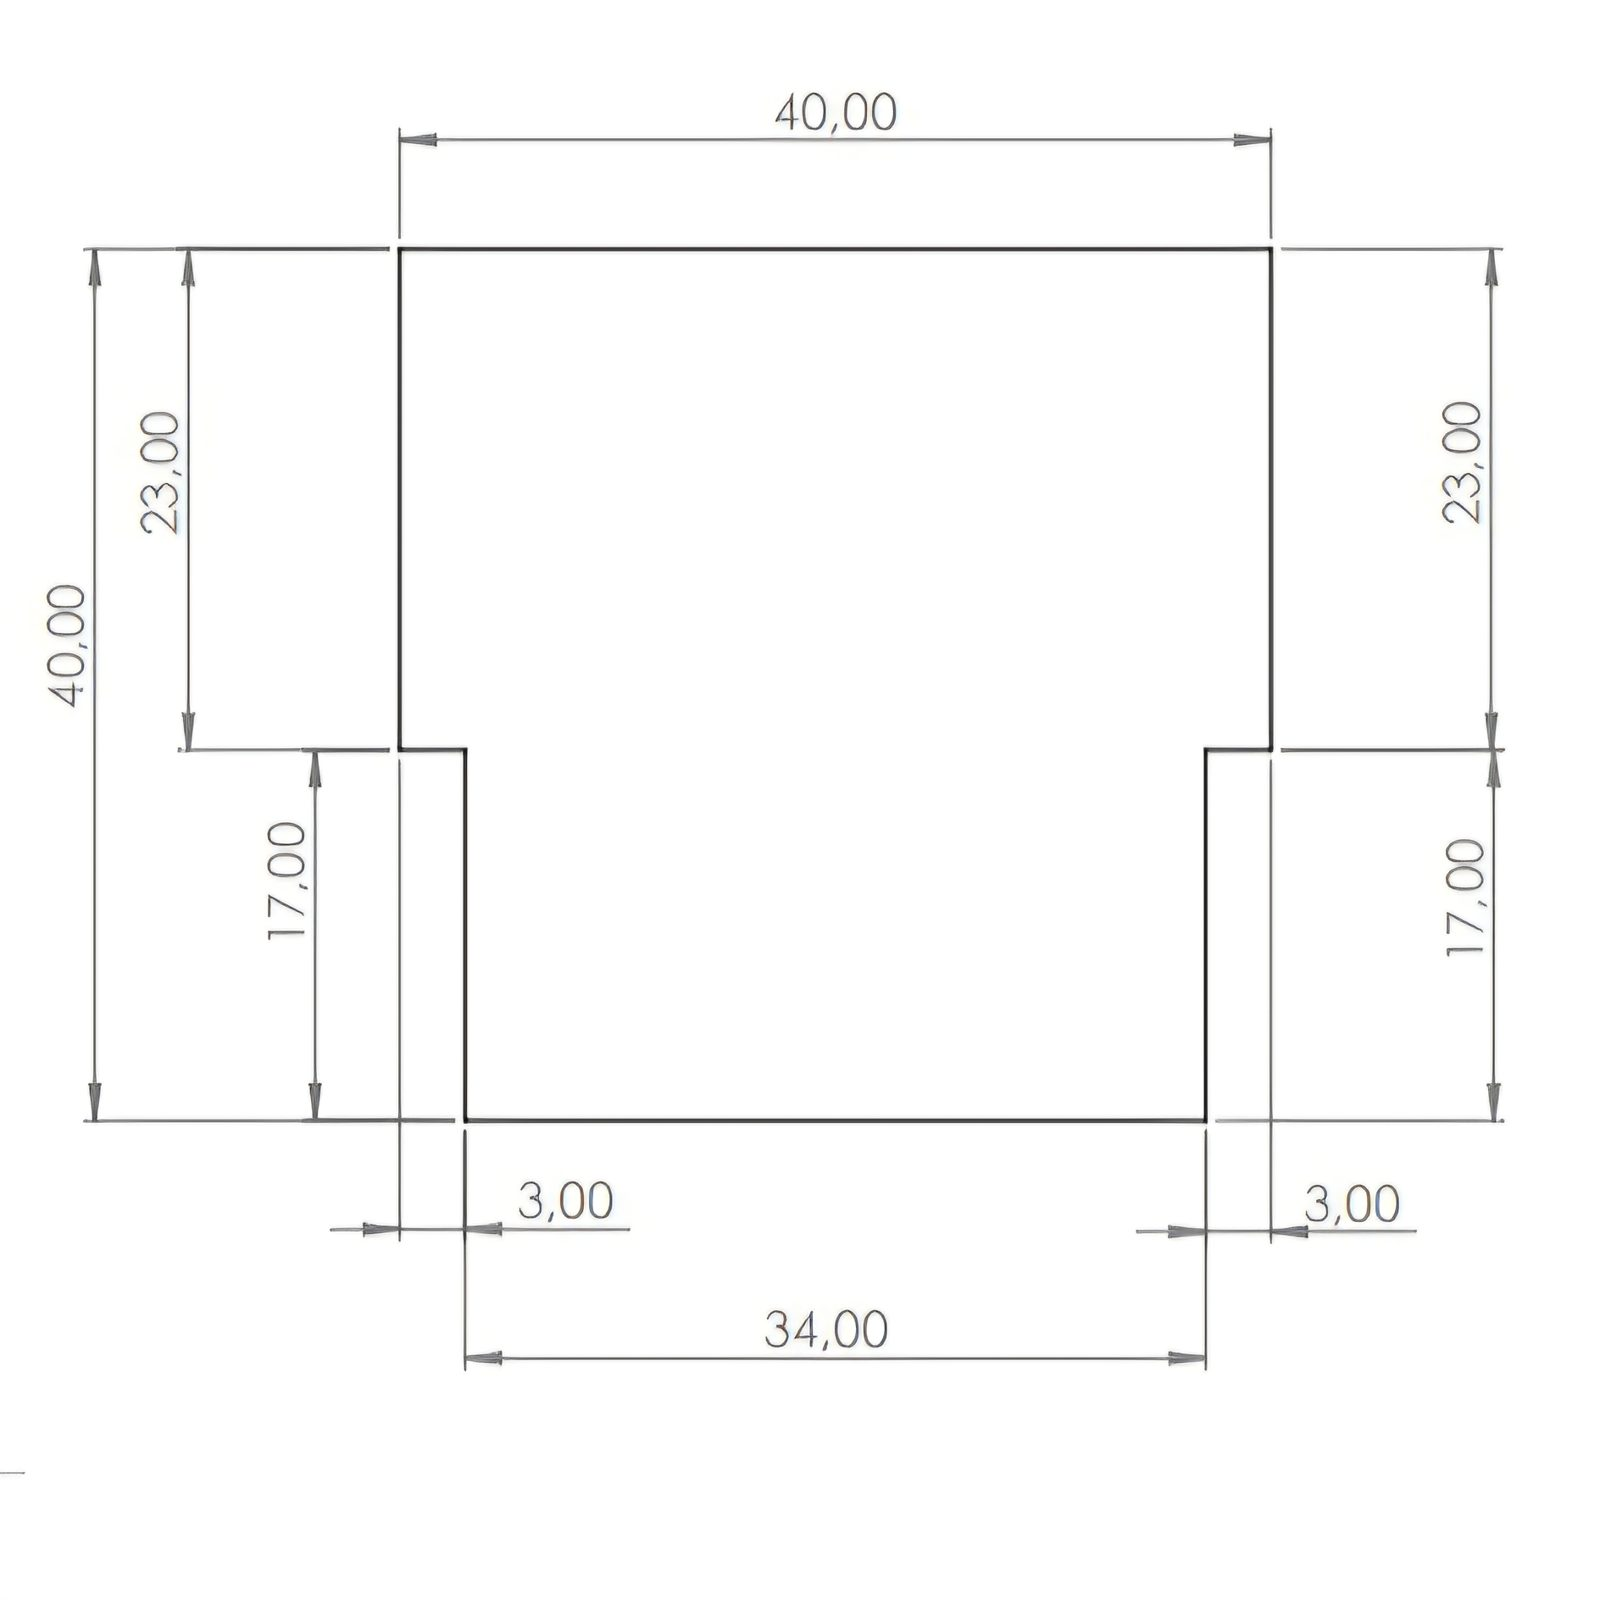
\includegraphics[width=\linewidth]{dimensiones_base.jpg}\caption{Planta de la tapa (cm).}\end{subfigure}\hfill
\begin{subfigure}{0.30\textwidth}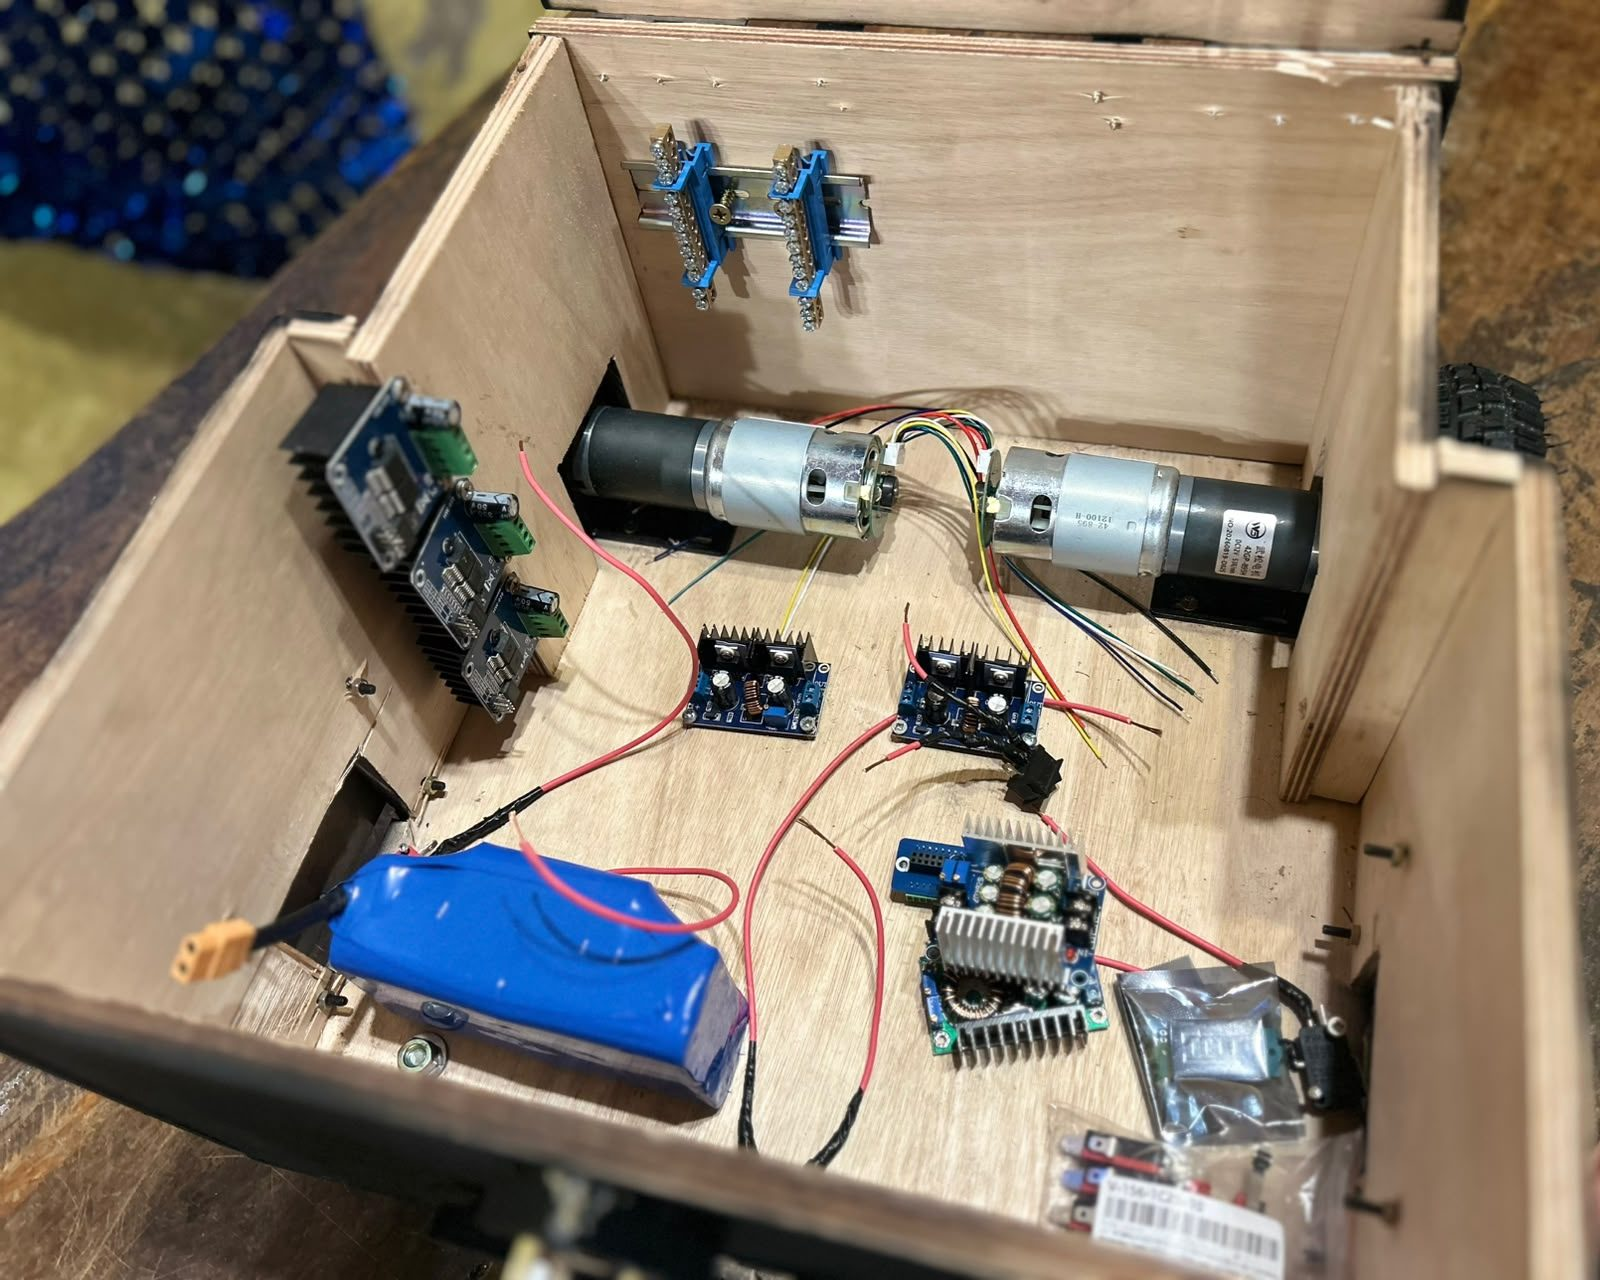
\includegraphics[width=\linewidth]{interior.jpg}\caption{Interior con la batería vieja.}\end{subfigure}\hfill
\begin{subfigure}{0.30\textwidth}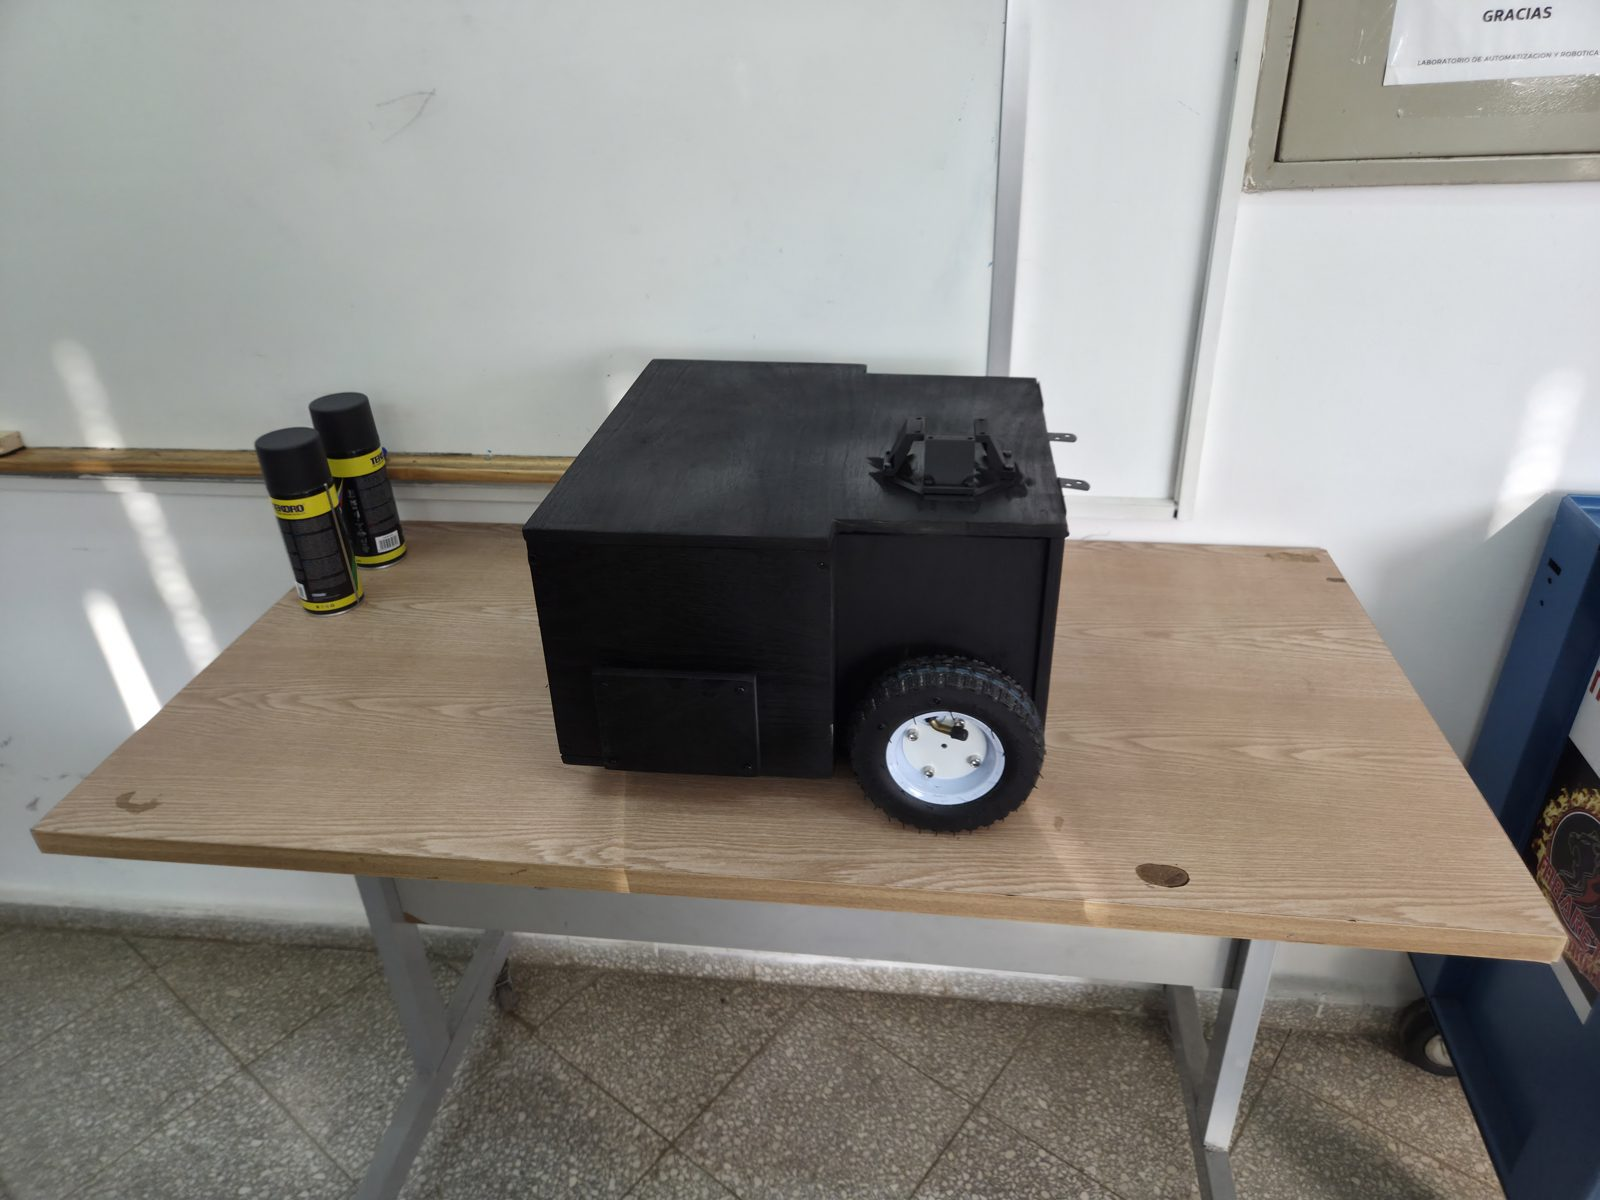
\includegraphics[width=\linewidth]{robot_izq.jpg}\caption{Vista lateral.}\end{subfigure}
\caption{La base de madera (entrega R2~E3).}
\end{figure}

\section{Tracción diferencial}

\subsection{Cómo se mueve un robot diferencial}
El robot tiene \textbf{dos ruedas motrices independientes} sobre el mismo eje y dos ruedas locas que solo apoyan.
No tiene dirección: para girar, una rueda va más rápido que la otra.

\begin{figure}[H]
\centering
\begin{tikzpicture}[scale=1.1]
  \draw[thick,fill=suave] (-1.2,-1) rectangle (1.2,1.4);
  \fill[tinta] (-1.45,-0.45) rectangle (-1.2,0.45); \fill[tinta] (1.2,-0.45) rectangle (1.45,0.45);
  \draw[dashed] (-1.6,0) -- (1.6,0);
  \fill[rojo] (0,0) circle (2pt);
  \draw[->,very thick,acento] (-1.33,0) -- (-1.33,1.0) node[above]{$v_i$};
  \draw[->,very thick,acento] (1.33,0) -- (1.33,1.6) node[above]{$v_d$};
  \draw[->,thick,rojo] (0,0) -- (0,1.3) node[above left]{$v$};
  \draw[->,thick,rojo] (0.5,0.2) arc (0:150:0.5) node[left]{$\omega$};
  \draw[<->] (-1.33,-1.3) -- node[below]{$b$ (trocha)} (1.33,-1.3);
  \node[align=left,anchor=west,font=\small] at (2.2,0.4) {
    $v = \dfrac{v_d + v_i}{2}$ \qquad $\omega = \dfrac{v_d - v_i}{b}$\\[10pt]
    $v_i = v - \omega\,\dfrac{b}{2}$ \qquad $v_d = v + \omega\,\dfrac{b}{2}$\\[10pt]
    $\text{rpm}_{i,d} = \dfrac{60\, v_{i,d}}{2\pi r}$};
\end{tikzpicture}
\caption{Cinemática diferencial. $v$ es la velocidad de avance del centro del eje [m/s], $\omega$ la velocidad de
giro [rad/s, positiva a la izquierda], $r = 0{,}075$~m el radio de rueda y $b = 0{,}40$~m la trocha (estimada:
\textbf{MEDIR}).}
\label{fig:diferencial}
\end{figure}

Ejemplos:
\begin{itemize}
  \item $v = 0{,}10$~m/s, $\omega = 0$: las dos ruedas a $\frac{60 \cdot 0{,}10}{2\pi \cdot 0{,}075} \approx 12{,}7$~rpm. Avanza recto.
  \item $v = 0$, $\omega = 0{,}5$~rad/s: $v_d = +0{,}10$, $v_i = -0{,}10$~m/s. Gira sobre su eje hacia la izquierda.
  \item $v = 0{,}10$, $\omega = 0{,}25$: $v_d = 0{,}15$, $v_i = 0{,}05$~m/s. Avanza curvando a la izquierda con radio
        $v/\omega = 0{,}4$~m.
\end{itemize}

Esto es lo que hace la clase \cod{Diferencial} del firmware de la base (\archivo{firmware/base/lib/BaseLogica/}): recibe
$(v, \omega)$ de \topic{/cmd\_vel}, calcula las rpm de cada rueda y, si alguna supera el máximo, \textbf{reduce las dos
en la misma proporción} para conservar la curvatura (el robot hace la misma curva, más despacio). Además aplica una
\textbf{rampa}: la velocidad cambia como mucho 0,3~m/s² y 1,5~rad/s², para que el robot no pegue tirones.

\subsection{Ruedas y motores de tracción}

\begin{figure}[H]
\centering
\begin{subfigure}{0.26\textwidth}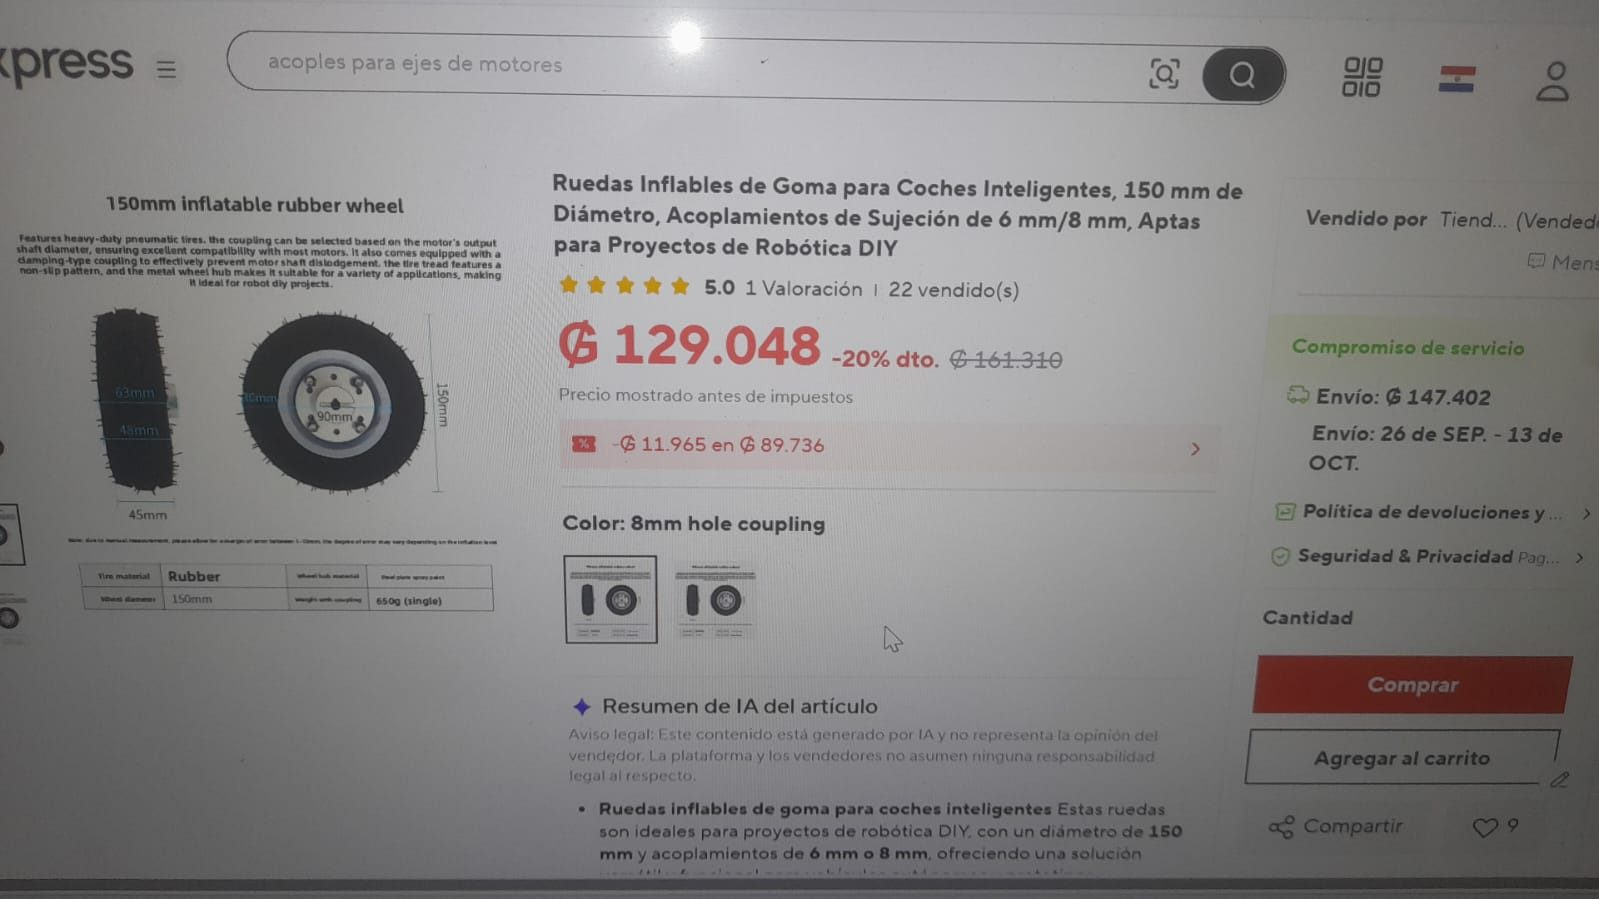
\includegraphics[width=\linewidth]{rueda.jpg}\caption{Rueda inflable de 150 mm.}\end{subfigure}\hfill
\begin{subfigure}{0.26\textwidth}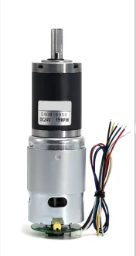
\includegraphics[width=\linewidth]{p_motor_traccion.jpg}\caption{42GM-895H con encoder.}\end{subfigure}\hfill
\begin{subfigure}{0.44\textwidth}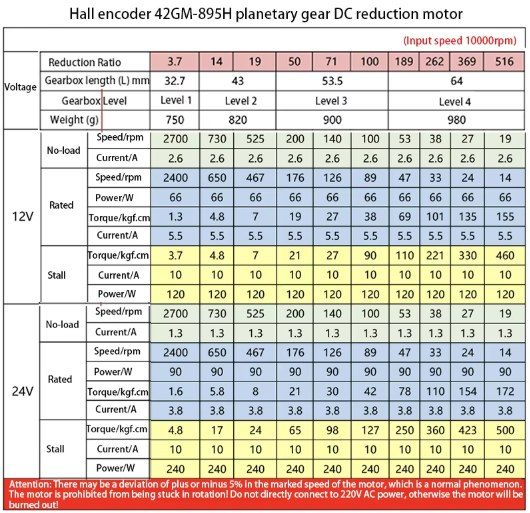
\includegraphics[width=\linewidth]{tabla_42gm.jpg}\caption{Hoja del vendedor (columna 189).}\end{subfigure}
\caption{Ruedas y motores de tracción.}
\end{figure}

\begin{center}
\begin{tabular}{@{}ll@{}}
\toprule
\textbf{Dato} & \textbf{Valor} \\
\midrule
Rueda & inflable, 150~mm de diámetro, 45~mm de ancho, 650~g \\
Motor & 42GM-895H planetario, 12~V, reducción 189:1 \\
Velocidad sin carga / nominal & 53~rpm / 47~rpm \\
Par nominal / trabado & 69~kgf·cm / 110~kgf·cm \\
Corriente sin carga / nominal / trabado & 2,6~A / 5,5~A / 10~A \\
Encoder & Hall, 11 pulsos por vuelta del motor, canales A y B, alimentado a 5~V \\
Cuentas por vuelta de la rueda & $11 \times 4 \times 189 = 8316$ (cuadratura ×4) \textbf{MEDIR} \\
Velocidad máxima teórica & $53 \cdot \pi \cdot 0{,}15 / 60 \approx 0{,}42$~m/s \\
Velocidad máxima configurada & 0,25~m/s y 1~rad/s (\cod{CFG\_DIF} en \archivo{base\_config.h}) \\
Velocidad de crucero del recorrido & 0,10~m/s \\
\bottomrule
\end{tabular}
\end{center}

\begin{nota}[Por qué se cuentan 4 flancos]
El encoder tiene dos canales, A y B, desfasados un cuarto de período. Contando los flancos de subida y de bajada de
los dos canales se obtienen 4 cuentas por pulso (``cuadratura ×4''), y el orden en que cambian A y B dice el
sentido de giro. El PCNT del ESP32 hace esto por hardware.
\end{nota}

\section{El brazo}

\subsection{Tipo y geometría}
El brazo es un manipulador \textbf{RRR} (tres articulaciones rotativas) del tipo \textbf{uArm / Dobot Magician}:
\begin{itemize}
  \item \textbf{J1 (base)} gira todo el brazo alrededor de un eje vertical.
  \item \textbf{J2 (hombro)} levanta la barra principal $L_2$.
  \item \textbf{J3 (codo)} mueve, a través de un \textbf{mecanismo de cuatro barras}, el antebrazo $L_3$. El motor
        de J3 está abajo, en la base del brazo, no en el codo: así el brazo es más liviano.
  \item Un \textbf{paralelogramo} mantiene la herramienta \textbf{siempre horizontal}, apuntando hacia afuera en
        la dirección de J1. Por eso basta con 3 motores para posicionar la pinza.
\end{itemize}

\begin{figure}[H]
\centering
\begin{tikzpicture}[scale=0.85]
  \fill[suave] (-1.5,-0.3) rectangle (1.5,0); \draw (-1.5,0) -- (1.5,0);
  \draw[very thick] (0,0) -- (0,1.5) node[midway,left]{$H_1 = 150$};
  \fill[tinta] (0,1.5) circle (3pt);
  \coordinate (B) at ($(0,1.5)+(50:3.5)$);
  \draw[line width=3pt,verde] (0,1.5) -- (B) node[midway,above left]{$L_2 = 350{,}2$};
  \fill[tinta] (B) circle (3pt);
  \coordinate (P) at ($(B)+(-20:3.3)$);
  \draw[line width=3pt,acento] (B) -- (P) node[midway,above right]{$L_3 = 329{,}5$};
  \fill[tinta] (P) circle (3pt) node[below]{muñeca $P_3$};
  \draw[line width=2pt,naranja] (P) -- ++(0.9,0) node[right]{TCP};
  \draw[dashed,gris] (0,1.5) -- (3,1.5);
  \draw[->] (1.2,1.5) arc (0:50:1.2) node[midway,right]{$q_2$};
  \draw[dashed,gris] (B) -- ($(B)+(50:1.5)$);
  \draw[->] ($(B)+(50:1.0)$) arc (50:-20:1.0) node[midway,right]{$q_{3O}$};
  % cuatro barras simplificado
  \draw[thick,rojo] (0,1.5) -- ++(-40:0.6) coordinate (r1);
  \draw[thick,ocre] (r1) -- ($(B)+(-110:0.6)$) node[midway,right,font=\scriptsize]{$L_4 = 338$};
  \draw[thick,rojo] (B) -- ($(B)+(-110:0.6)$);
  \node[font=\scriptsize,rojo] at (-0.2,0.85) {balancín};
  \draw[->,thick] (-1.0,0.3) arc (200:340:1.0 and 0.3) node[right]{$q_1$};
  \node[align=left,font=\small,anchor=west] at (6.6,2.6) {Medidas en mm (entrega R1~E4):\\
    $H_1 = 150$ (altura del hombro)\\ $L_2 = 350{,}22$ (barra verde)\\ $L_3 = 329{,}51$ (antebrazo)\\
    $L_4 = 338$ (acoplador)\\ $L_{3,0} = L_{3,1} = 40$ (balancines)\\[4pt]
    Rangos:\\ $q_1 \in [45^\circ, 225^\circ]$\\ $q_2 \in [-25^\circ, 135^\circ]$\\ $q_3 \in [-50^\circ, 50^\circ]$};
\end{tikzpicture}
\caption{Esquema lateral del brazo (no a escala). El motor de J3 mueve el balancín rojo de abajo; el acoplador
amarillo transmite el movimiento al codo. $q_{3O}$, el ángulo del antebrazo respecto de la prolongación de $L_2$, es
una consecuencia de $q_2$ y $q_3$ por el cierre del cuatro barras.}
\label{fig:brazo}
\end{figure}

\begin{pendiente}[Balancín del cuatro barras]
\archivo{cinematica.py} usa balancines de 40~mm (E4). Según \archivo{ARQUITECTURA.md} §11, el balancín rojo se
cambió a \textbf{60~mm} el 03/10 para que el mecanismo sea de Grashof. Verificar la medida real y, si cambió,
actualizar \cod{L30} en \archivo{ros2\_ws/src/brazo\_ik/brazo\_ik/cinematica.py} y volver a correr sus pruebas.
\end{pendiente}

\subsection{Dónde va montado y qué alcanza}
El brazo va \textbf{atrás a la izquierda, sobre el eje de tracción}, a unos 6~cm del costado ($y = 0{,}11$~m,
preliminar). $q_1 = 0$ apunta hacia adelante y crece en sentido antihorario visto desde arriba. El rango de J1
($45^\circ$ a $225^\circ$) va de adelante-izquierda, pasando por la izquierda y por atrás, hasta atrás-derecha: \textbf{nunca
cruza el mástil de las cámaras}, que está adelante a la derecha. $q_1 = 90^\circ$ (brazo hacia el costado izquierdo) es
la marca del banco de pruebas y la pose de cero de J1.

La consigna de R1 define la zona de trabajo como una esfera de 30~cm de diámetro centrada a unos 35~cm del suelo.
Con el robot centrado en el pasillo de la simulación, los limones quedan a unos 0,45~m del eje de J1.

\subsection{Motores y transmisiones}

\begin{center}
\begin{tabular}{@{}lccc@{}}
\toprule
 & \textbf{J1 (base)} & \textbf{J2 (hombro)} & \textbf{J3 (codo)} \\
\midrule
Motor & 36GP-555, 160~rpm & 36-555, 58~rpm & 36-555, 58~rpm \\
Reductora del motor & 50:1 & 139:1 & 139:1 \\
Transmisión & correa GT2 18 → 90 (5:1) & helicoidales 15 → 75 (5:1) & helicoidales 15 → 75 (5:1) \\
Velocidad máx. de la articulación & 32~rpm (192~°/s) & 11,6~rpm (70~°/s) & 11,6~rpm (70~°/s) \\
Encoder & \multicolumn{3}{c}{SCX-555, 16 pulsos por vuelta, cuadratura ×4, alimentado a \textbf{3,3~V}} \\
Cuentas por vuelta de la articulación & $3200 \times 5 = 16\,000$ & $8896 \times 5 = 44\,480$ & $44\,480$ \\
Resolución & 44,4 cuentas/° & 123,6 cuentas/° & 123,6 cuentas/° \\
Corriente (vacío / nominal / trabado) & \multicolumn{3}{c}{0,5~A / 1,3~A / 10~A a 12~V} \\
Se autobloquea & no & \textbf{no} & \textbf{no} \\
Estado & medido (02/10) & llega 19--29/10 & llega 19--29/10 \\
\bottomrule
\end{tabular}
\end{center}

\begin{peligro}[J2 y J3 no se sostienen solos]
Los motores planetarios de J2 y J3 \textbf{no se autobloquean}: sin corriente, el brazo cae por su peso. Pasa al
apretar la seta, al desarmar en rueda libre o al cortar los 12~V. Dejar siempre el brazo en reposo \textbf{apoyado en
un tope} y no poner las manos debajo. Falta resolver cómo sostenerlo (contrapeso o resorte con lo que haya).
\end{peligro}

\begin{figure}[H]
\centering
\begin{subfigure}{0.24\textwidth}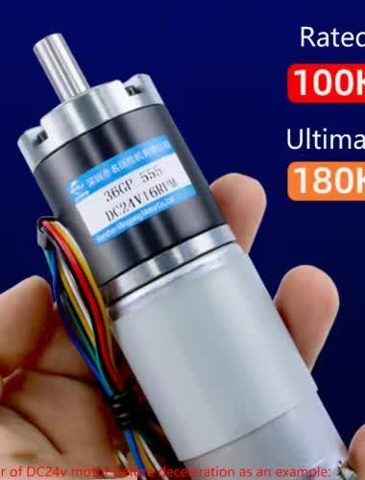
\includegraphics[width=\linewidth]{p_motor_brazo.jpg}\caption{36GP-555 con encoder.}\end{subfigure}\hfill
\begin{subfigure}{0.24\textwidth}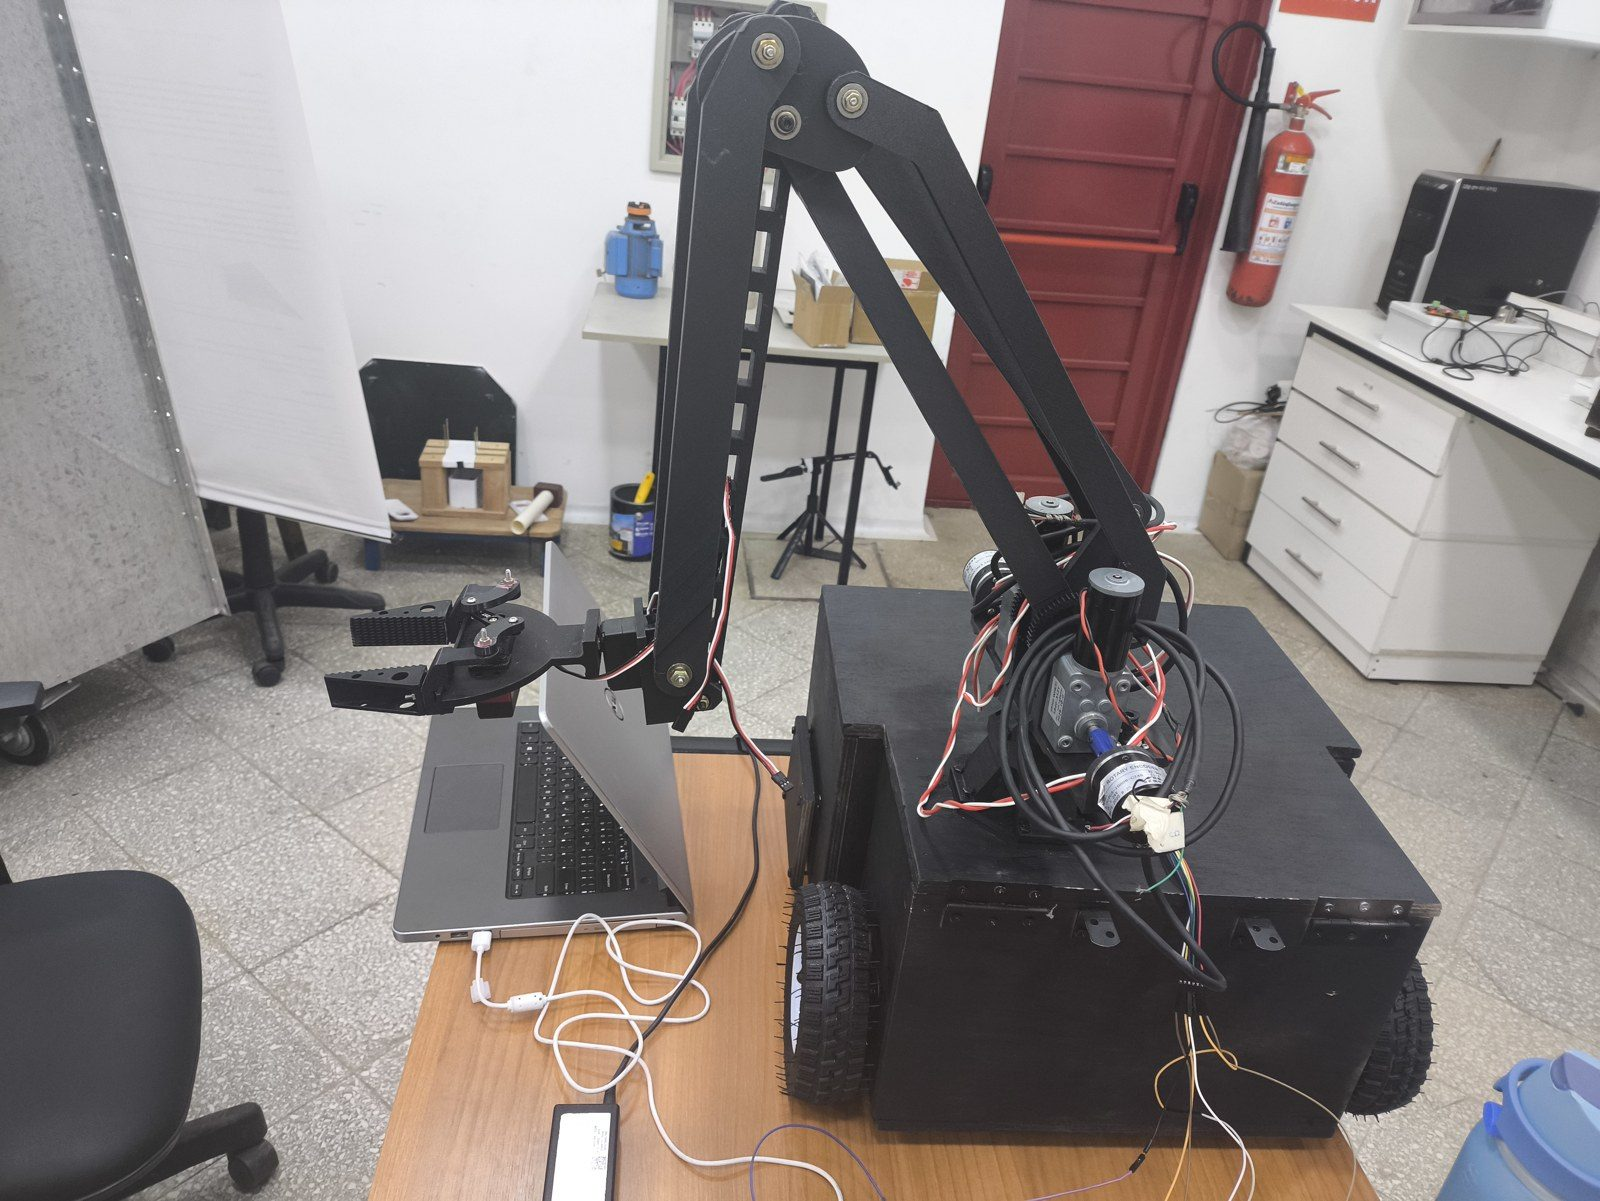
\includegraphics[width=\linewidth]{brazo_j1_cero.jpg}\caption{J1 en su cero.}\end{subfigure}\hfill
\begin{subfigure}{0.24\textwidth}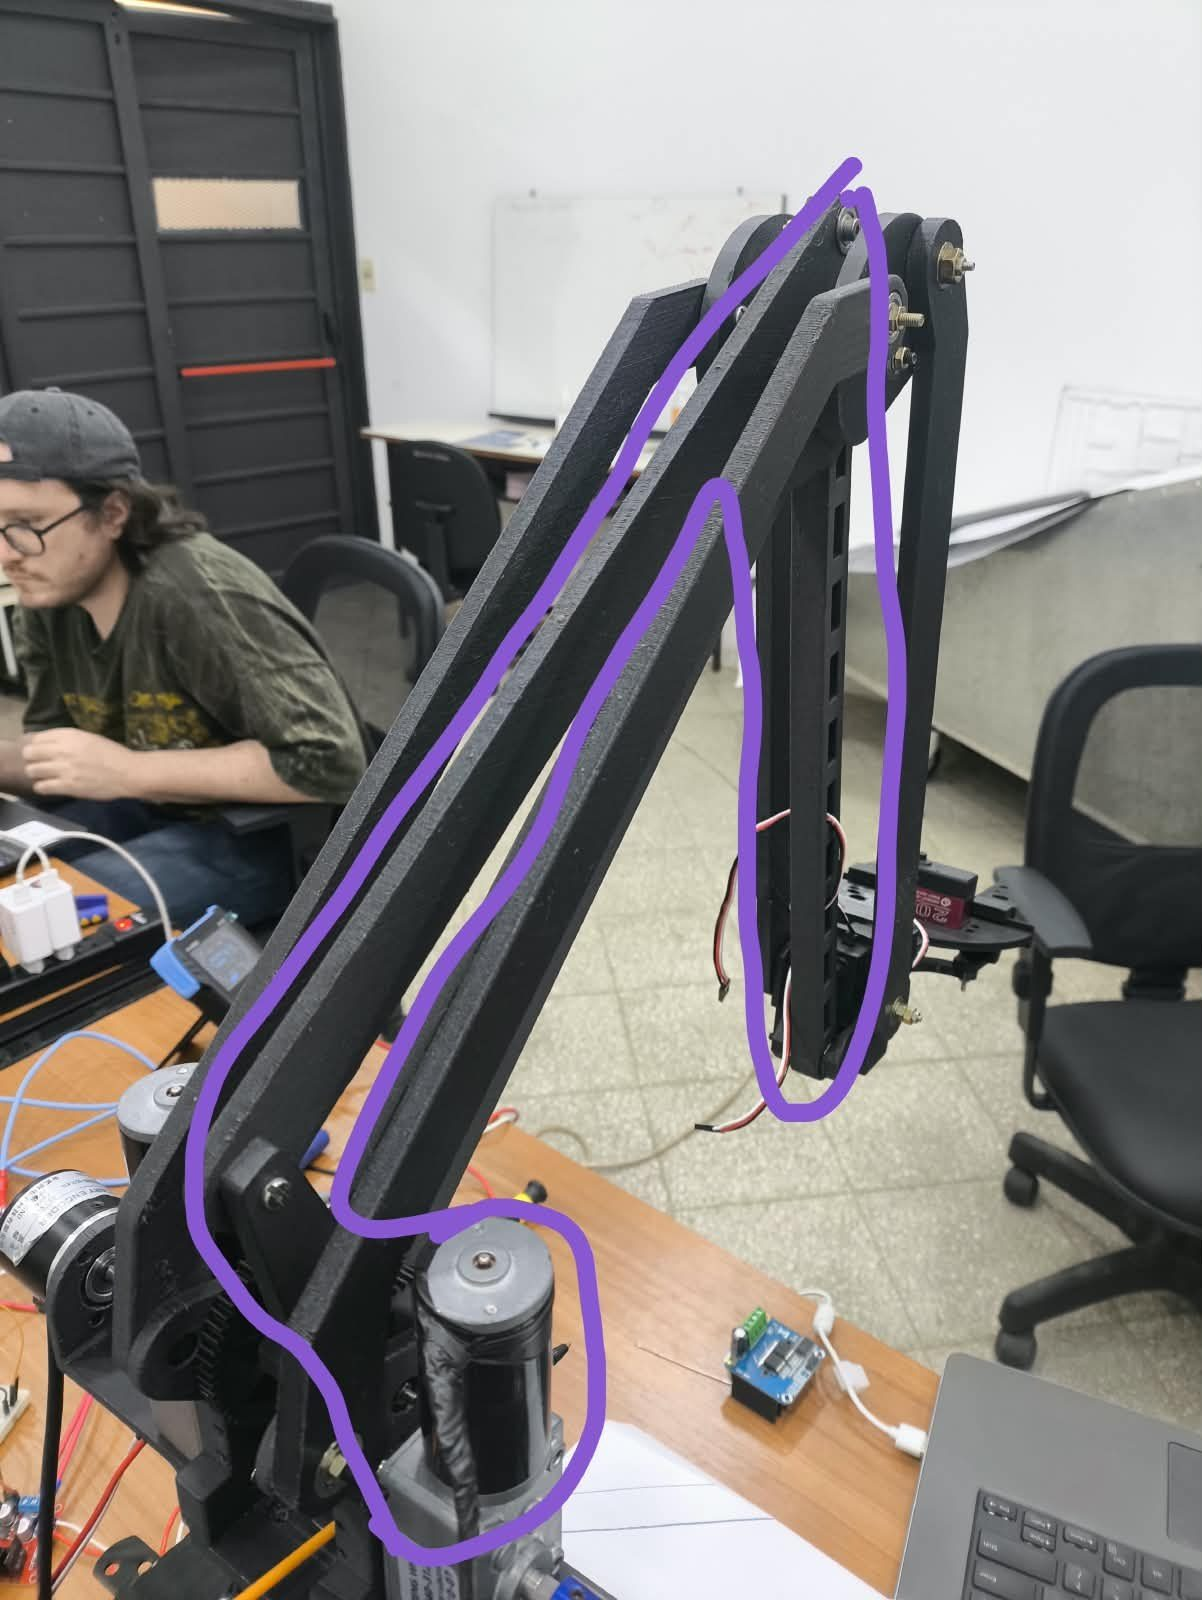
\includegraphics[width=\linewidth]{brazo_codo_j3.jpg}\caption{Cuatro barras del codo.}\end{subfigure}\hfill
\begin{subfigure}{0.24\textwidth}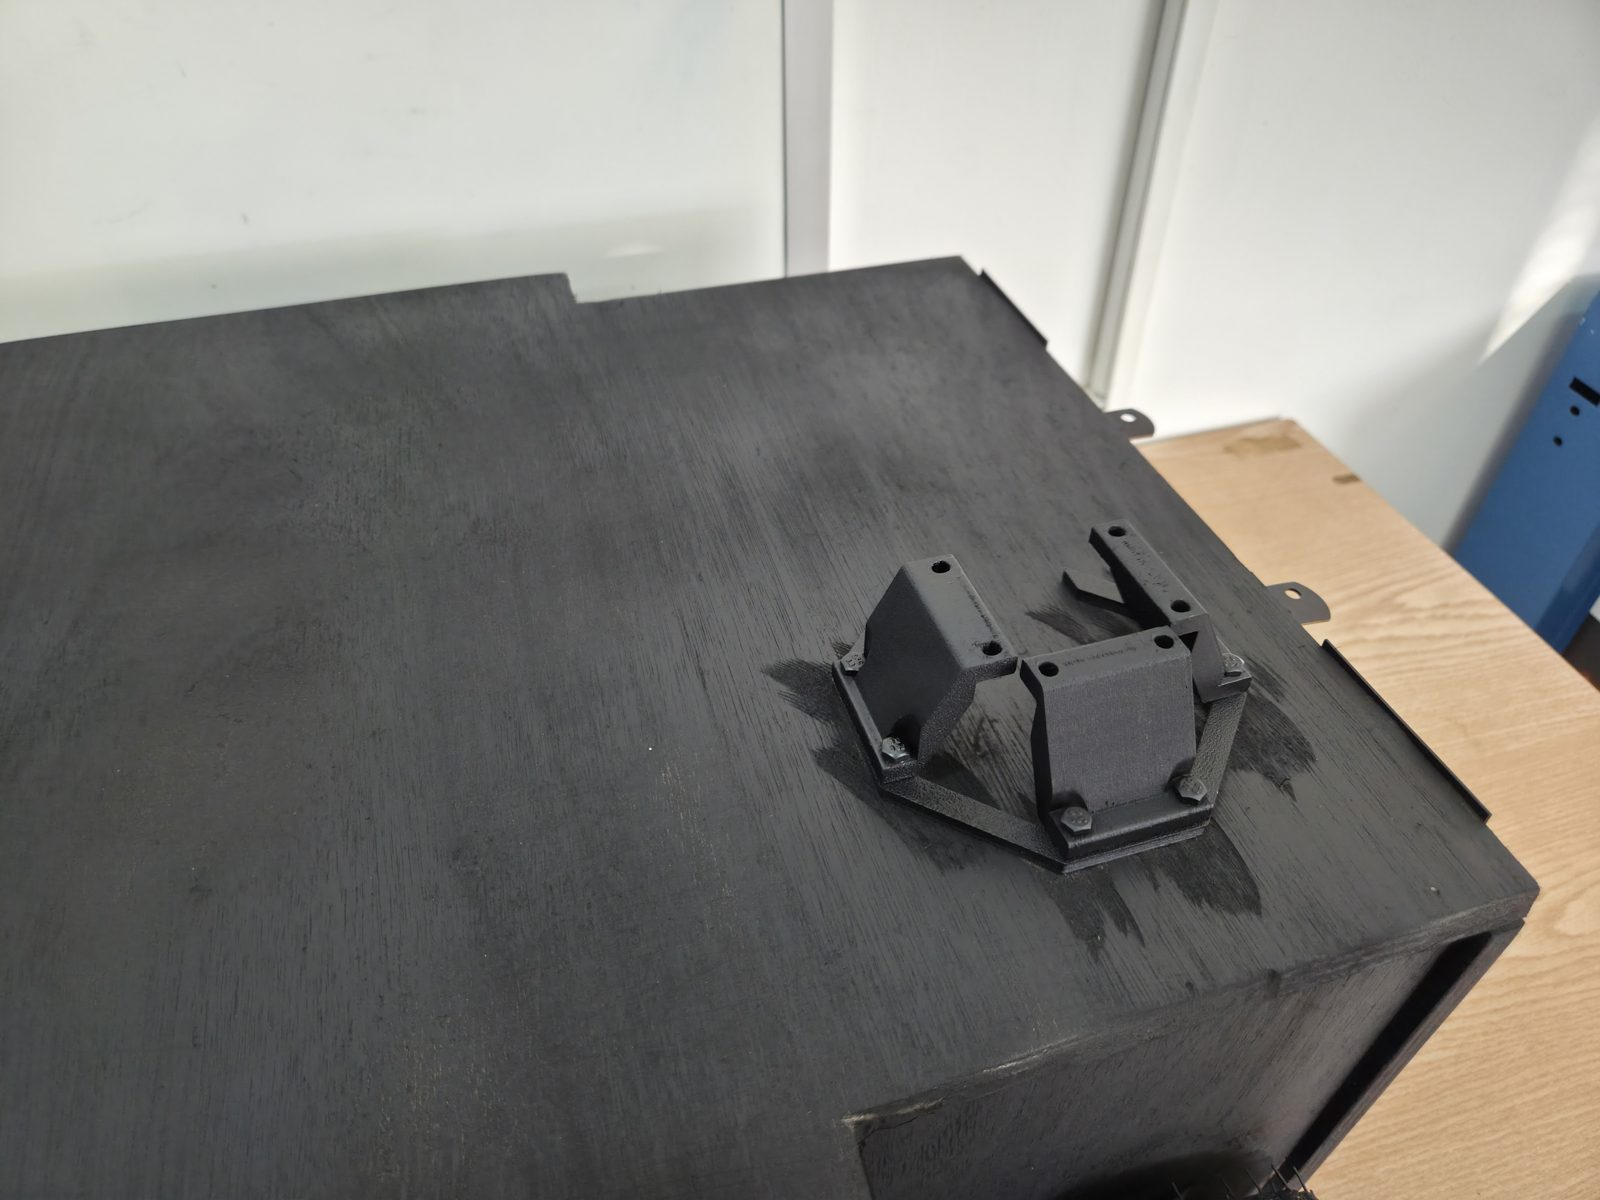
\includegraphics[width=\linewidth]{base_brazo.jpg}\caption{Base impresa del brazo.}\end{subfigure}
\caption{Motores y partes del brazo.}
\end{figure}

Colores de los cables de los 36GP-555: \textbf{blanco} = motor +, \textbf{amarillo} = motor −, \textbf{verde} =
encoder + (a 3,3~V), \textbf{azul} = GND, \textbf{negro} = canal A, \textbf{rojo} = canal B. El encoder tiene salida de
colector abierto con pull-up de 5,1~kΩ en su plaquita: alimentado a 3,3~V, sus salidas quedan en 0 o 3,3~V, que el
ESP32 tolera.

\section{La pinza}

La pinza tiene dos servos \textbf{DSSERVO RDS3218} de 20~kg·cm, alimentados con 6~V por el buck~3:
\begin{itemize}
  \item \textbf{Apertura} (GPIO~4 de la WROOM): 0~\% = abierta, 100~\% = cerrada (\topic{/pinza/cierre}).
  \item \textbf{Giro J4} (GPIO~14): rota la pinza alrededor del eje de la herramienta, de $-90^\circ$ a $+90^\circ$
        (\topic{/pinza/giro}). Sirve para desprender el limón retorciendo el pedúnculo.
\end{itemize}
La cosecha es: \textbf{agarrar} (cerrar), \textbf{traccionar} (retroceder 1--2~cm), \textbf{girar} J4 y
\textbf{retirar}. Hoy la misión hace solo agarrar y retirar; el giro queda para después.

\begin{figure}[H]
\centering
\begin{subfigure}{0.28\textwidth}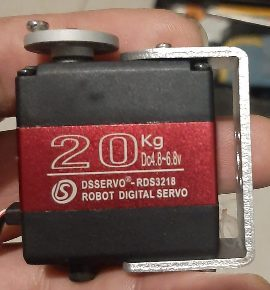
\includegraphics[width=\linewidth]{p_servo.jpg}\caption{Servo RDS3218.}\end{subfigure}\hspace{8mm}
\begin{subfigure}{0.28\textwidth}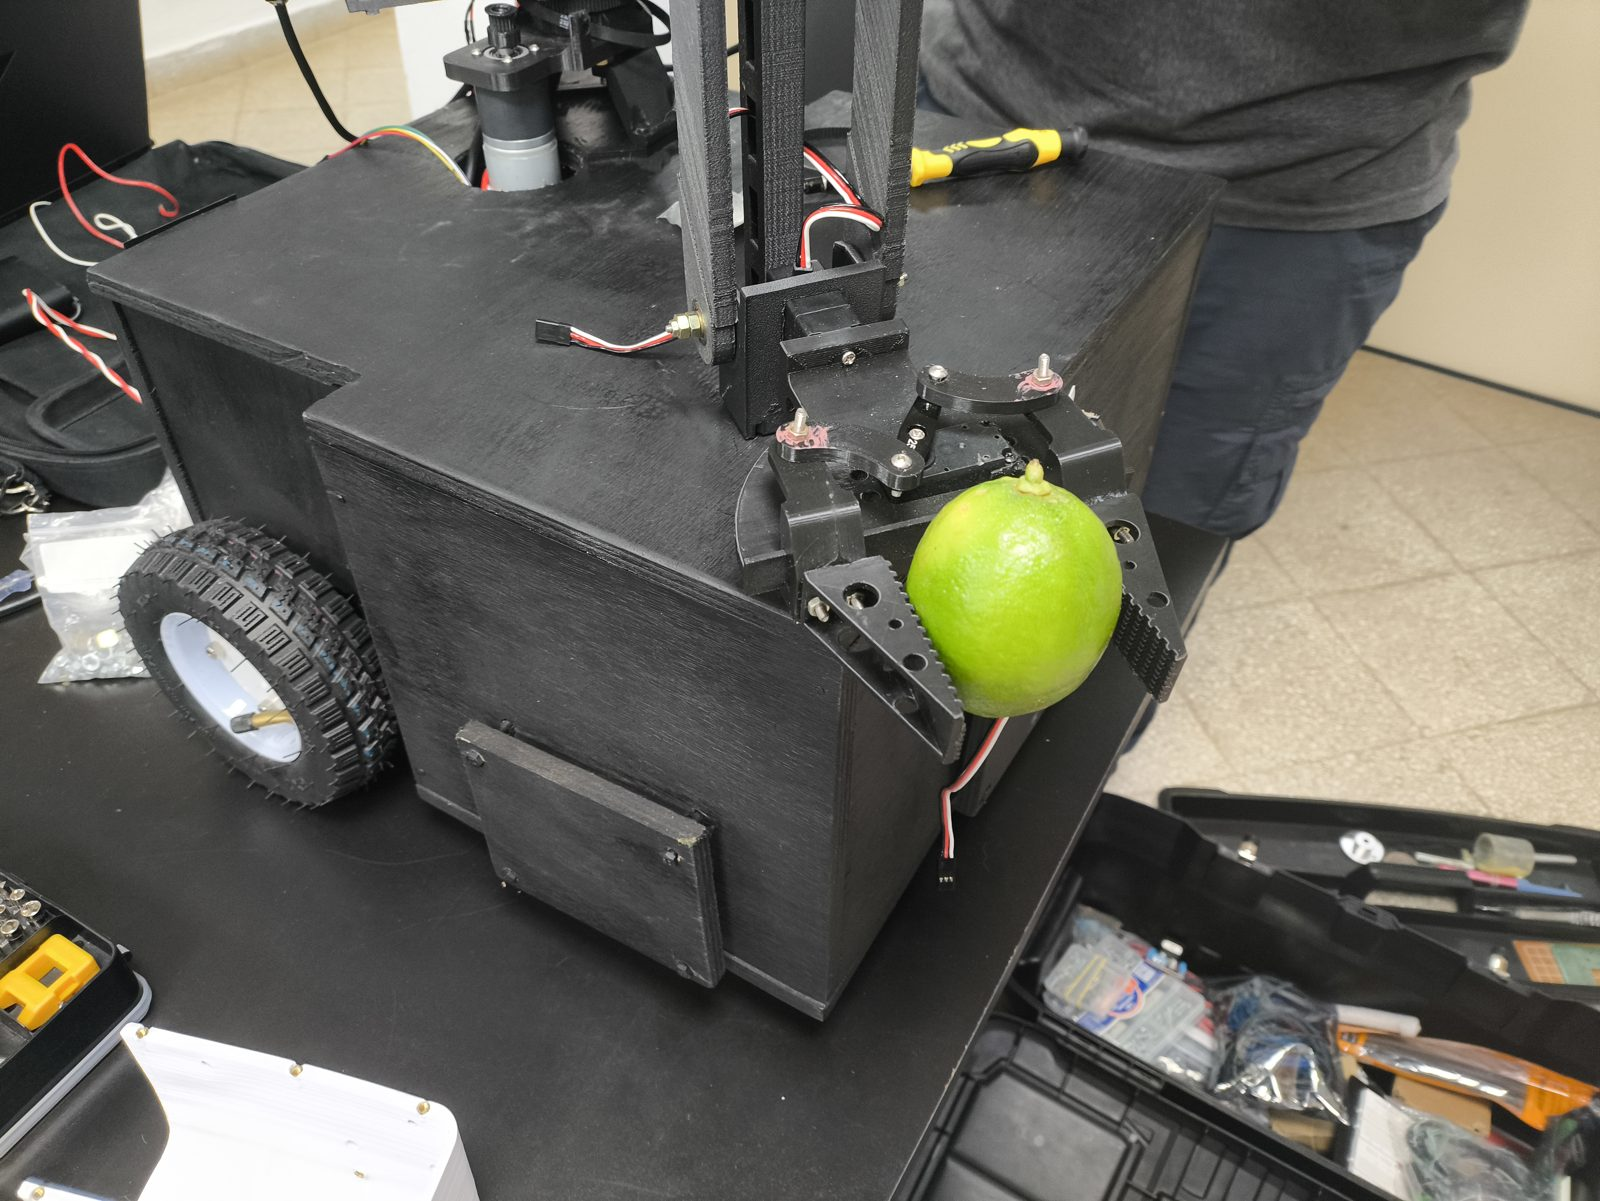
\includegraphics[width=\linewidth]{robot_limon.jpg}\caption{Pinza con un limón.}\end{subfigure}
\caption{La pinza.}
\end{figure}

\begin{pendiente}
Pulsos reales de cada servo (\cod{PINZA\_US\_*}, \cod{GIRO\_US\_*}), el porcentaje de cierre que agarra sin aplastar
(\cod{cierre} en la misión) y \cod{largo\_herramienta}: la distancia horizontal de la muñeca al centro del agarre
(capítulo~\ref{cap:ik}).
\end{pendiente}

\chapter{Alimentación y potencia}\label{cap:potencia}

\section{Dos fuentes separadas}

El robot tiene \textbf{dos fuentes de energía que nunca se tocan} (salvo el GND común):

\begin{description}
  \item[LiPo 3S para los motores] 11,1~V nominal (9,9--12,6~V), 8000~mAh (88,8~Wh). Alimenta los cinco IBT-2 y el
        buck de los servos. Los motores son de 12~V y el IBT-2 acepta de 5,5 a 27~V, así que la LiPo va
        \textbf{directa, sin convertidor}.
  \item[Power bank para la lógica] Xiaomi PB2030MI, 5~V 3~A por su cable USB-C. Alimenta la Raspberry Pi, y la Pi
        alimenta los dos ESP32 por USB.
\end{description}

\begin{idea}[Por qué separadas]
Un motor trabado puede pedir 10~A y hacer caer la tensión de la batería. Si la Pi estuviera en la misma batería,
se reiniciaría en medio de una cosecha. Con fuentes separadas, aunque los motores se queden sin energía (seta,
fusible, batería baja), la Pi y los ESP32 siguen encendidos y saben lo que pasó.
\end{idea}

\section{El circuito, paso a paso}

\begin{figure}[H]
\centering
\resizebox{\textwidth}{!}{%
\begin{tikzpicture}[node distance=5mm]
  \node[caja,draw=rojo,thick] (lipo) {LiPo 3S\\8000 mAh\\sin BMS};
  \node[caja,right=of lipo] (xt) {XT60};
  \node[caja,right=of xt,draw=rojo] (fus) {fusible de\\auto 20 A};
  \node[caja,right=of fus] (sel) {selector WEG\\2 NA en paralelo\\(ON/OFF)};
  \node[caja,right=of sel,draw=violeta,thick] (seta) {seta\\bloque A (NC)};
  \node[caja,right=12mm of seta,minimum height=58mm,text width=18mm,fill=rojo!8] (bus) {bornera\\+12 V\\[18mm]bornera\\GND};
  \draw[pot] (lipo) -- (xt); \draw[pot] (xt) -- (fus); \draw[pot] (fus) -- (sel); \draw[pot] (sel) -- (seta); \draw[pot] (seta) -- (bus);
  \node[caja,right=14mm of bus,yshift=22mm] (t) {2 × IBT-2 de tracción};
  \node[caja,right=14mm of bus,yshift=10mm] (b) {3 × IBT-2 del brazo};
  \node[caja,right=14mm of bus,yshift=-2mm] (bk) {buck 3 → 6 V → 2 servos};
  \node[caja,right=14mm of bus,yshift=-14mm] (dv) {divisor 100 k / 30 k → S3 GPIO 1};
  \node[caja,right=14mm of bus,yshift=-26mm] (cap) {capacitores ≥ 25 V};
  \foreach \n in {t,b,bk,dv,cap} \draw[pot] (bus.east |- \n) -- (\n);
  \node[caja,below=10mm of lipo,font=\scriptsize] (ind) {indicador de barras\\(conector de balanceo)};
  \draw[->,gris] (lipo) -- (ind);
  \node[caja,draw=naranja,thick,below=26mm of xt] (pb) {power bank\\5 V 3 A};
  \node[caja,right=of pb] (pi) {Raspberry Pi 5};
  \node[caja,right=of pi] (esp) {ESP32-S3 y WROOM\\(por USB)};
  \draw[logica] (pb) -- (pi); \draw[logica] (pi) -- node[topico,above]{USB} (esp);
  \node[caja,draw=violeta,below=of seta,yshift=-6mm] (setab) {seta bloque B (NC)};
  \draw[seg] (setab) |- node[topico,pos=0.7,above]{GPIO 47} (esp.east);
  \draw[violeta,dashed] (seta) -- node[topico,right]{mismo botón} (setab);
  \draw[thick,tinta] (esp.south) -- ++(0,-0.5) -| node[topico,pos=0.25,below]{GND común (un cable de cada placa)} (bus.south);
\end{tikzpicture}}
\caption{Circuito de potencia (v0.7, 10/10). Rojo: 12~V de motores. Naranja: 5~V de lógica. Violeta: seguridad.}
\label{fig:potencia}
\end{figure}

\begin{figure}[H]
\centering
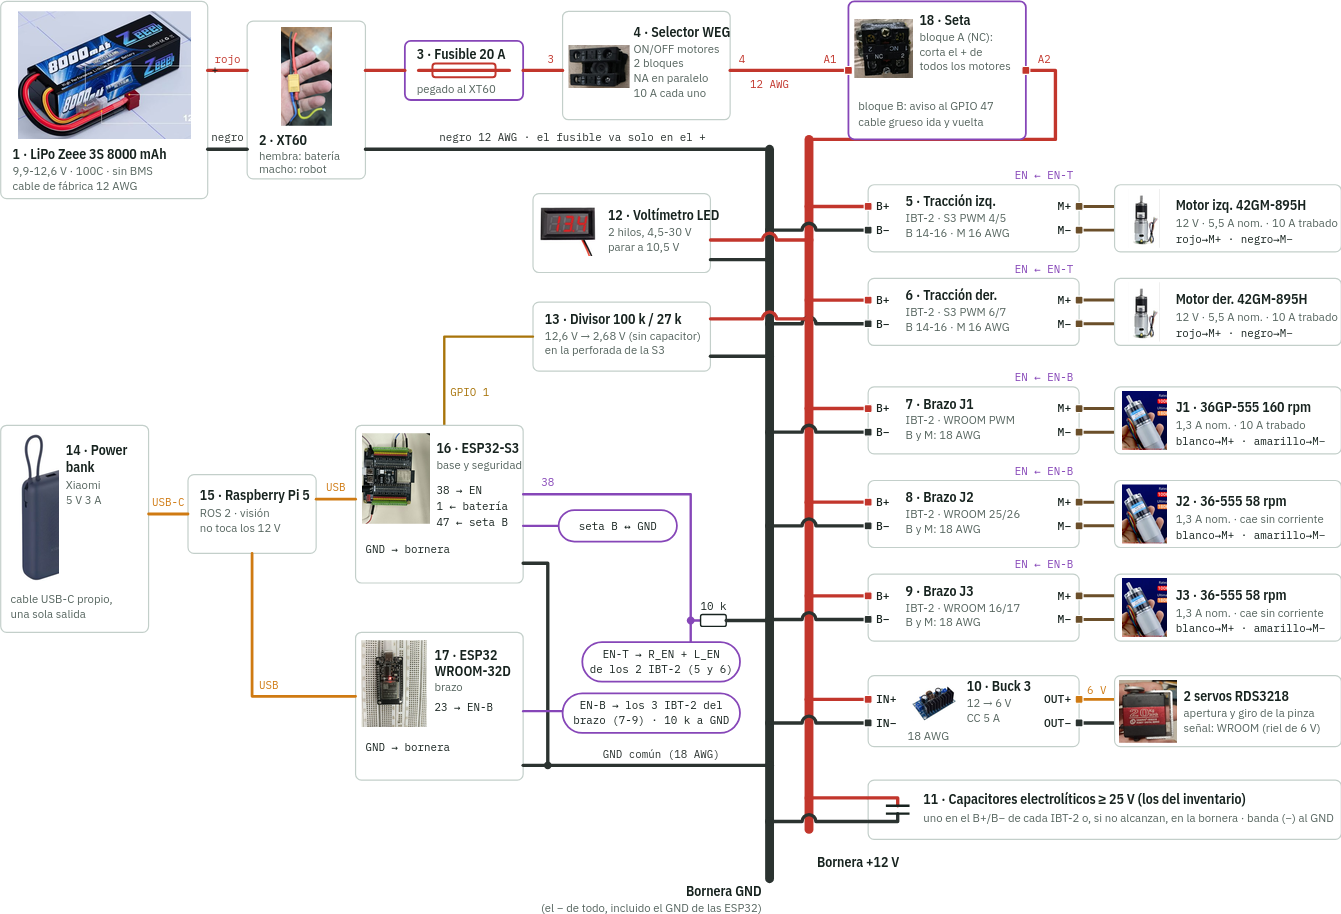
\includegraphics[width=\textwidth]{html_potencia.png}
\caption{Cableado de potencia completo, con fotos y calibres (de \archivo{docs/html/potencia.html}). Los números
coinciden con las fichas de la sección~\ref{sec:piezas}.}
\end{figure}

\section{Cada pieza}\label{sec:piezas}

\begin{figure}[H]
\centering
\begin{subfigure}{0.19\textwidth}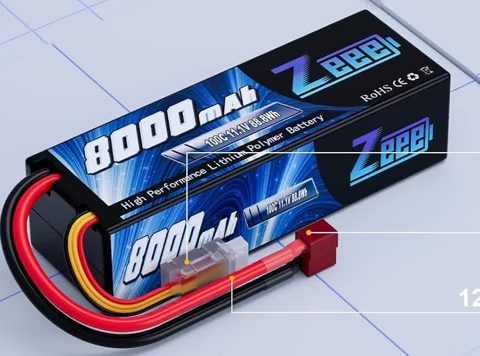
\includegraphics[width=\linewidth,height=3cm,keepaspectratio]{p_lipo.jpg}\caption{LiPo 3S}\end{subfigure}\hfill
\begin{subfigure}{0.19\textwidth}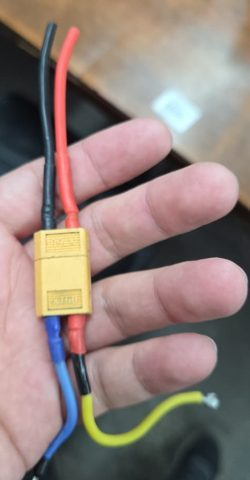
\includegraphics[width=\linewidth,height=3cm,keepaspectratio]{p_xt60.jpg}\caption{XT60}\end{subfigure}\hfill
\begin{subfigure}{0.19\textwidth}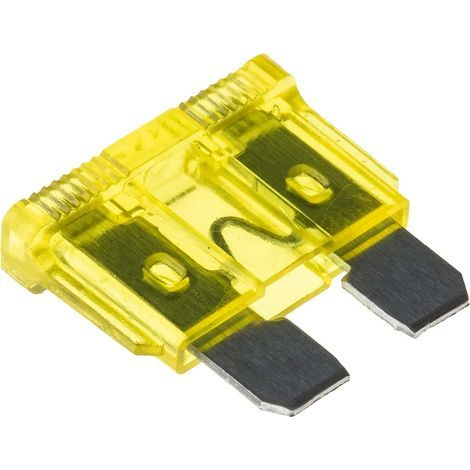
\includegraphics[width=\linewidth,height=3cm,keepaspectratio]{fusible.jpg}\caption{Fusible 20 A}\end{subfigure}\hfill
\begin{subfigure}{0.19\textwidth}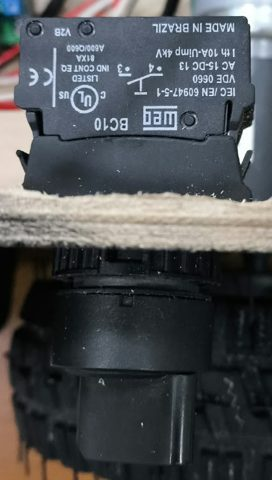
\includegraphics[width=\linewidth,height=3cm,keepaspectratio]{p_selector.jpg}\caption{Selector WEG}\end{subfigure}\hfill
\begin{subfigure}{0.19\textwidth}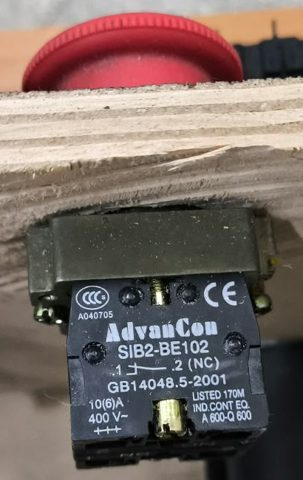
\includegraphics[width=\linewidth,height=3cm,keepaspectratio]{p_seta.jpg}\caption{Seta}\end{subfigure}\\[4pt]
\begin{subfigure}{0.19\textwidth}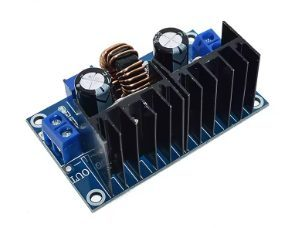
\includegraphics[width=\linewidth,height=3cm,keepaspectratio]{p_buck3.jpg}\caption{Buck 3}\end{subfigure}\hfill
\begin{subfigure}{0.19\textwidth}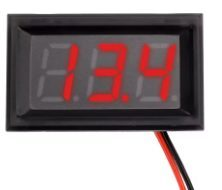
\includegraphics[width=\linewidth,height=3cm,keepaspectratio]{p_voltimetro.jpg}\caption{Voltímetro}\end{subfigure}\hfill
\begin{subfigure}{0.19\textwidth}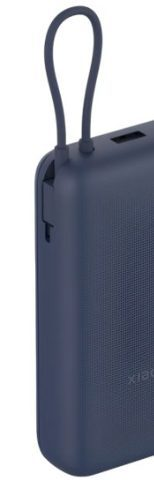
\includegraphics[width=\linewidth,height=3cm,keepaspectratio]{p_powerbank.jpg}\caption{Power bank}\end{subfigure}\hfill
\begin{subfigure}{0.19\textwidth}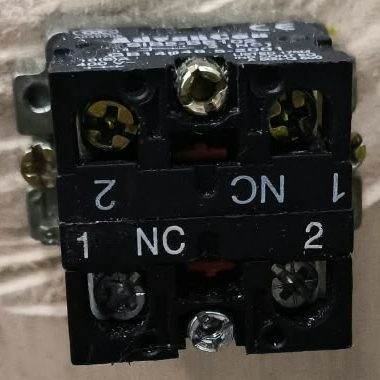
\includegraphics[width=\linewidth,height=3cm,keepaspectratio]{p_hongo_atras.jpg}\caption{Seta, atrás}\end{subfigure}\hfill
\begin{subfigure}{0.19\textwidth}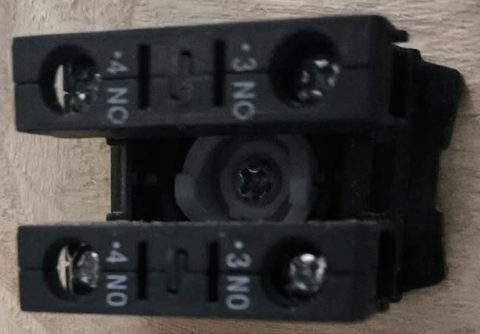
\includegraphics[width=\linewidth,height=3cm,keepaspectratio]{p_selector_atras.jpg}\caption{Selector, atrás}\end{subfigure}
\caption{Las piezas del circuito de potencia.}
\end{figure}

\begin{longtable}{@{}p{3.3cm} p{12.2cm}@{}}
\toprule
\textbf{Pieza} & \textbf{Qué hace y cómo se usa} \\
\midrule
\endhead
LiPo Zeee 3S & 11,1~V, 8000~mAh, 100C, 493~g. \textbf{No tiene BMS}: nada la protege de la sobredescarga. Se carga
  solo con el cargador balanceador y fuera del robot. Guardada varios días, a $\sim$11,4~V (3,8~V por celda). Su
  conector Deans de fábrica se cambia por un \textbf{XT60} (no hay Deans hembra). \\
XT60 & Conector de la batería. Se enchufa \textbf{con el selector en OFF} y respetando la polaridad: los IBT-2 al
  revés se rompen. Al cambiar el Deans, cortar \textbf{de a un cable} (los dos juntos con la pinza hacen un corto). \\
Fusible de auto 20~A & Lámina ATO/ATC, apto para continua hasta 32~V. Va \textbf{pegado al XT60}: el cable antes
  del fusible no está protegido. \textbf{Protege contra cortocircuitos}; no salta con dos motores trabados
  ($2 \times 10$~A es justo su nominal). Cable del bus de al menos 14~AWG. \\
Selector WEG & ON/OFF diario de los motores. Dos bloques BC10 normalmente abiertos en paralelo. \textbf{Moverlo solo
  con los motores quietos}: dos contactos en paralelo no suman 20~A al abrir (el último en separarse corta todo). \\
Seta (bloque A) & Contacto normalmente cerrado en serie con el + del bus de 12~V, después del selector. Al apretarla,
  los cinco IBT-2 y el buck quedan sin tensión. Los motores quedan en rueda libre: \textbf{no frena}. Está pensada
  para alterna (\cod{10(6)A 400V\textasciitilde}): solo para emergencias. \\
Seta (bloque B) & Otro contacto NC del mismo botón, entre el GPIO~47 de la S3 y GND. Avisa al firmware. \textbf{Nunca
  12~V en este bloque}: queman el GPIO. \\
IBT-2 (×5) & Puentes H BTS7960: 2 de tracción y 3 del brazo. Entrada de potencia B+/B−, salida al motor M+/M−. \\
Buck 3 & XL4016 (4--38~V de entrada, 5~A). Baja 12~V a 6~V para los servos, con límite de corriente en 5~A.
  \textbf{Ajustarlo sin carga y con el multímetro} antes de conectar los servos. \\
Capacitores & Electrolíticos de $\geq 25$~V cerca de los IBT-2, para absorber picos. \\
Divisor 100~k / 30~k & Baja 12,6~V a 2,91~V para el ADC del GPIO~1 de la S3. Si alguna vez vuelve la batería 10S
  (36~V), \textbf{cambiarlo antes a 120~k / 8,2~k}: con 42~V el de 30~k pondría $\sim$9~V en el GPIO y lo quema. \\
Voltímetro / indicador & Muestra la tensión a la vista. Parar a 10,5~V. \\
Power bank & 20\,000~mAh, 5~V 3~A. Una sola salida, cable incorporado (corto), arriba al lado de la Pi. No cargarlo
  mientras alimenta la Pi (puede cortar un instante). \\
\bottomrule
\end{longtable}

\section{Consumo y autonomía}

\begin{center}
\begin{tabular}{@{}lr@{}}
\toprule
\textbf{Carga} & \textbf{Potencia} \\
\midrule
Tracción avanzando a 0,25~m/s ($2 \times 60\% \times 12\text{ V} \times 3\text{ A}$) & $\sim$43~W \\
Tracción girando o en terreno malo & $\sim$70~W \\
Brazo moviéndose (J1--J3 + servos) & $\sim$26~W \\
Brazo quieto sosteniendo (J2/J3 contra el peso + pinza) & $\sim$6~W \\
Lógica: Pi 5 con YOLO ($\sim$9~W), ESP32 (0,8~W), sensores (0,6~W) & $\sim$11~W \\
\bottomrule
\end{tabular}
\end{center}

Ciclo de cosecha de un limón (60~s): 20~s avanzando, 5~s maniobrando, 25~s con el brazo en movimiento y 10~s con el
brazo quieto:
\[
P_\text{motores} = \frac{20\,(43 + 6) + 5\,(70 + 6) + 25 \cdot 26 + 10 \cdot 6}{60} \approx 34{,}5\text{ W}
\]
Con el 80~\% de la energía nominal como útil (71~Wh):

\begin{figure}[H]
\centering
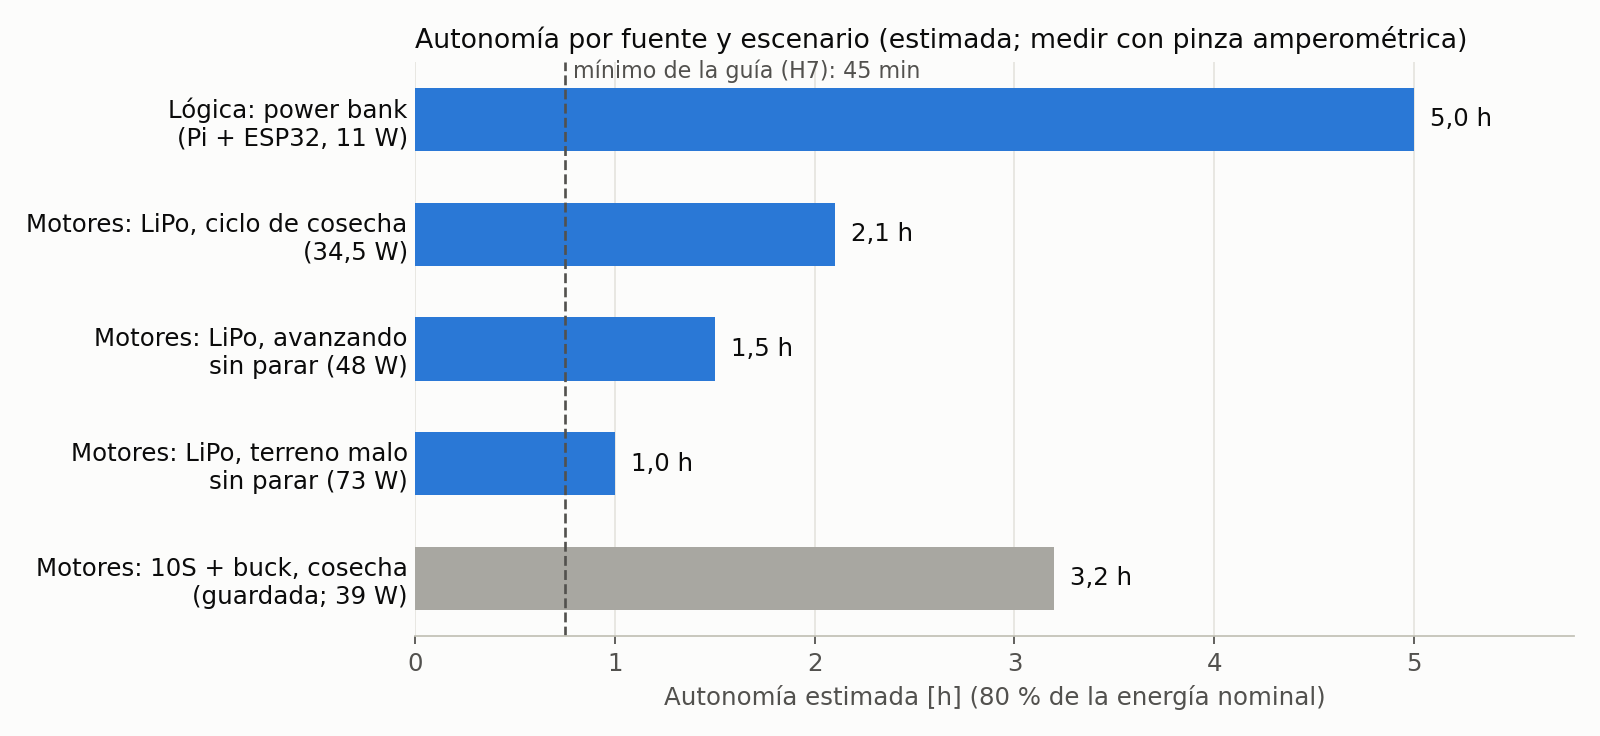
\includegraphics[width=0.85\textwidth]{autonomia.png}
\caption{Autonomía estimada por fuente y escenario (de la entrega R2~E4). La guía pide al menos 45~min. El robot
dura lo que dura la LiPo: $\sim$2,1~h de cosecha.}
\end{figure}

\section{La batería sin BMS}

\begin{peligro}[La LiPo no se protege sola]
\begin{itemize}[leftmargin=*]
  \item El firmware de la base mide la tensión y avisa \cod{BATERIA\_BAJA} a 10,5~V en \topic{/base/estado}, pero
        \textbf{no frena}: hay que parar a mano.
  \item 10,5~V en total no garantizan 3,5~V en cada celda. Ni el ADC ni el indicador ven una celda desbalanceada.
        \textbf{Medir cada celda} con el balanceador o el tester antes y después de cada prueba.
  \item Calibrar la lectura del ADC contra el tester.
  \item Con la seta apretada, el divisor marca 0~V (\cod{BATERIA\_BAJA}): es normal.
\end{itemize}
\end{peligro}

\section{Reglas para las pruebas}

La revisión de Codex del 14/10 confirmó que el conexionado está bien, pero que varios componentes no tienen
garantizado cortar con carga en continua. Por eso las pruebas son \textbf{acotadas y vigiladas}:

\begin{enumerate}
  \item Mover el selector \textbf{solo con los motores quietos}.
  \item Si se aprieta la seta, \textbf{mandar \cod{desarmar} al brazo y confirmar que quedó desarmado antes de
        soltarla} (aunque \cod{mision} esté corriendo).
  \item \textbf{Nada de pruebas de motores trabados con la LiPo}: el fusible no salta con eso. Usar una fuente
        limitada en corriente.
  \item Cables a las borneras con \textbf{cobre pelado y retorcido, sin estañar}: el estaño cede bajo el tornillo.
  \item Siempre alguien con la mano en la seta o en el selector.
  \item Apagar los 12~V antes de flashear o resetear un ESP32 (al reiniciar, los pines quedan un instante sin
        control).
\end{enumerate}

\chapter{Placas, pines y cableado}\label{cap:placas}

\section{Vista general del cableado}

\begin{figure}[H]
\centering
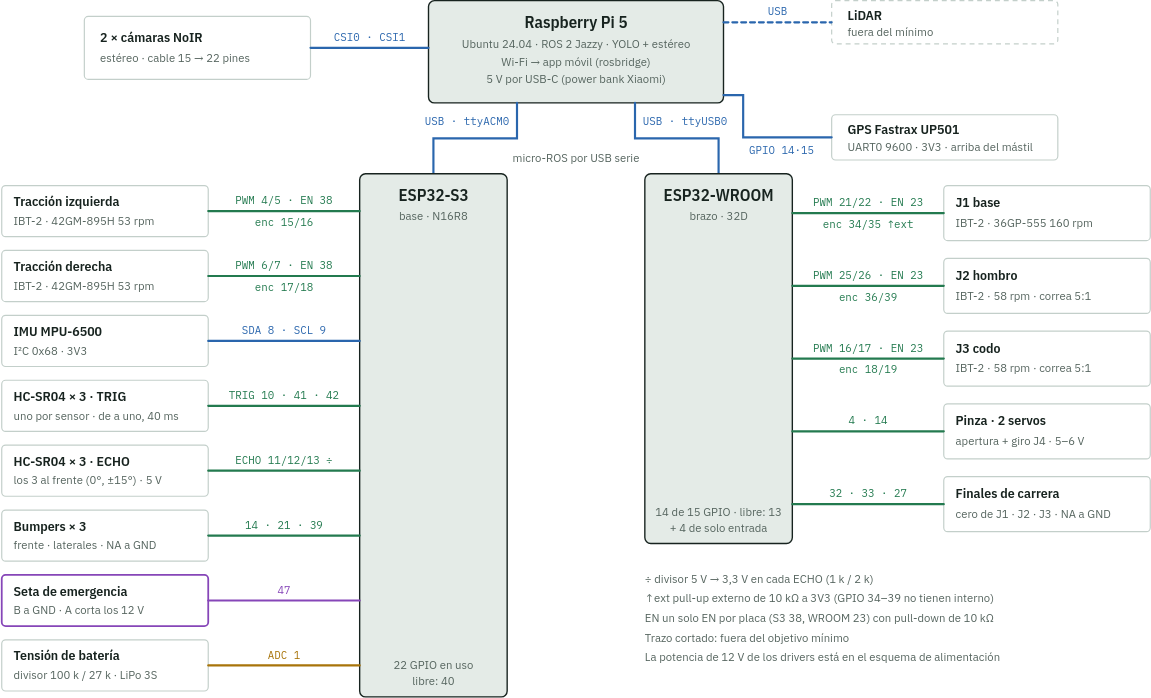
\includegraphics[width=\textwidth]{html_general.png}
\caption{Qué va conectado a qué, con el número de GPIO en cada cable (de \archivo{docs/html/conexiones.html}).
Azul: datos (USB, CSI, I²C, UART). Verde: GPIO y PWM. Ocre: analógico. Violeta: seguridad.}
\end{figure}

\begin{nota}[Dónde está la verdad]
Los pines \textbf{solo} se definen en \archivo{firmware/base/include/pins.h} y \archivo{firmware/brazo/include/pins.h}.
\archivo{docs/CONEXIONES.md} y las páginas de \archivo{docs/html/} los copian. Si hay una diferencia, manda
\cod{pins.h}. Las páginas HTML son interactivas: \archivo{docs/html/todo.html} junta todas, con cajas clickeables.
\end{nota}

\section{Tres ideas eléctricas que aparecen en todas partes}

\subsection{Los GPIO del ESP32 son de 3,3~V}
Un pin del ESP32 se rompe si recibe más de 3,6~V. Hay tres cosas en el robot que sacan 5~V: el ECHO de los HC-SR04,
los encoders de tracción y (si vuelve la 10S) la batería. Todas pasan por un \textbf{divisor resistivo}:
\[
V_\text{GPIO} = V_\text{entrada}\,\frac{R_\text{abajo}}{R_\text{arriba} + R_\text{abajo}}
\]
\begin{itemize}
  \item ECHO del HC-SR04: 1~kΩ arriba y 2~kΩ abajo: $5 \cdot \frac{2}{3} = 3{,}33$~V.
  \item Encoders de tracción: tienen un pull-up interno de 10~kΩ a 5~V; se agrega 20~kΩ a GND: $5 \cdot \frac{20}{30} = 3{,}33$~V.
  \item Batería: 100~kΩ arriba y 27~kΩ abajo: $12{,}6 \cdot \frac{27}{127} = 2{,}68$~V (el ADC lee hasta $\sim$3,1~V).
\end{itemize}

\subsection{Pull-up y pull-down}
Un pin de entrada ``al aire'' lee cualquier cosa. Un \textbf{pull-up} (resistencia a 3,3~V) lo deja en 1 cuando nada
lo conecta; el interruptor lo lleva a 0 conectándolo a GND. Así funcionan los bumpers, la seta y los finales de
carrera: \textbf{apretado = LOW}. El ESP32 tiene pull-ups internos, \textbf{salvo los GPIO 34 a 39 de la WROOM}, que
son solo de entrada y no tienen: ahí van los encoders, que traen su propio pull-up de 5,1~kΩ.

Un \textbf{pull-down} hace lo contrario. Los EN de los IBT-2 tienen uno de 10~kΩ: mientras el ESP32 arranca o se
reinicia, sus pines flotan; el pull-down mantiene los puentes deshabilitados y los motores quietos.

\subsection{La seta es normalmente cerrada (falla segura)}
El bloque B de la seta une el GPIO~47 con GND cuando está suelta. Al apretarla, o si \textbf{se corta un cable}, el pin
sube a HIGH por el pull-up y la S3 entra en EMERGENCIA. Un cable cortado se comporta como una seta apretada: es más
seguro que al revés.

\section{ESP32-S3: la base}

Placa Freenove ESP32-S3-WROOM N16R8, con USB nativo (aparece en la Pi como \cod{/dev/ttyACM0}). Va encima de una
\textbf{placa de expansión Freenove} con una bornera por pin, y los componentes (resistencias) van en dos perforadas
chicas, una sobre cada fila de borneras. Desde el 13/10 \textbf{no lleva capacitores}: bumpers y seta van directo.

{\small\begin{longtable}{@{}p{2.6cm} p{6.6cm} p{6.4cm}@{}}
\toprule
\textbf{GPIO} & \textbf{Conecta a} & \textbf{Nota} \\
\midrule
\endhead
4 · 5 & IBT-2 izquierdo RPWM · LPWM & PWM a 20~kHz, 10 bits \\
6 · 7 & IBT-2 derecho RPWM · LPWM & 20~kHz \\
38 & R\_EN + L\_EN de los dos IBT-2 & pull-down 10~kΩ \\
15 · 16 & Encoder izquierdo A · B & amarillo · blanco; 20~kΩ a GND \\
17 · 18 & Encoder derecho A · B & amarillo · blanco; 20~kΩ a GND \\
8 · 9 & IMU SDA · SCL & I²C 400~kHz, dirección 0x68 \\
10 · 41 · 42 & TRIG del HC-SR04 frente · izquierda · derecha & disparados de a uno, cada 40~ms \\
11 · 12 · 13 & ECHO frente · izquierda · derecha & divisor 1~k / 2~k \\
14 · 21 · 39 & Bumpers frente · izquierda · derecha & NA a GND, pull-up interno \\
47 & Seta, bloque B (NC) & a GND; HIGH = apretada o cable cortado \\
1 & Divisor de batería 100~k / 27~k & ADC1 canal 0 \\
40 & libre & reservado para un 4.º bumper \\
\bottomrule
\end{longtable}}

Prohibidos en la S3: 19/20 (USB), 26--37 (memoria flash y PSRAM). Evitar: 0/3/45/46 (\textit{strapping}: definen el
modo de arranque), 43/44 (UART0), 2/48 (LED).

\begin{pendiente}[LED RGB de la S3]
En la DevKitC-1 v1.1 el LED RGB está en el GPIO~38, que es el EN de la tracción. \cod{pins.h} supone el 48. Verificar
la placa real y no usar nunca el LED RGB en el firmware.
\end{pendiente}

\begin{figure}[H]
\centering
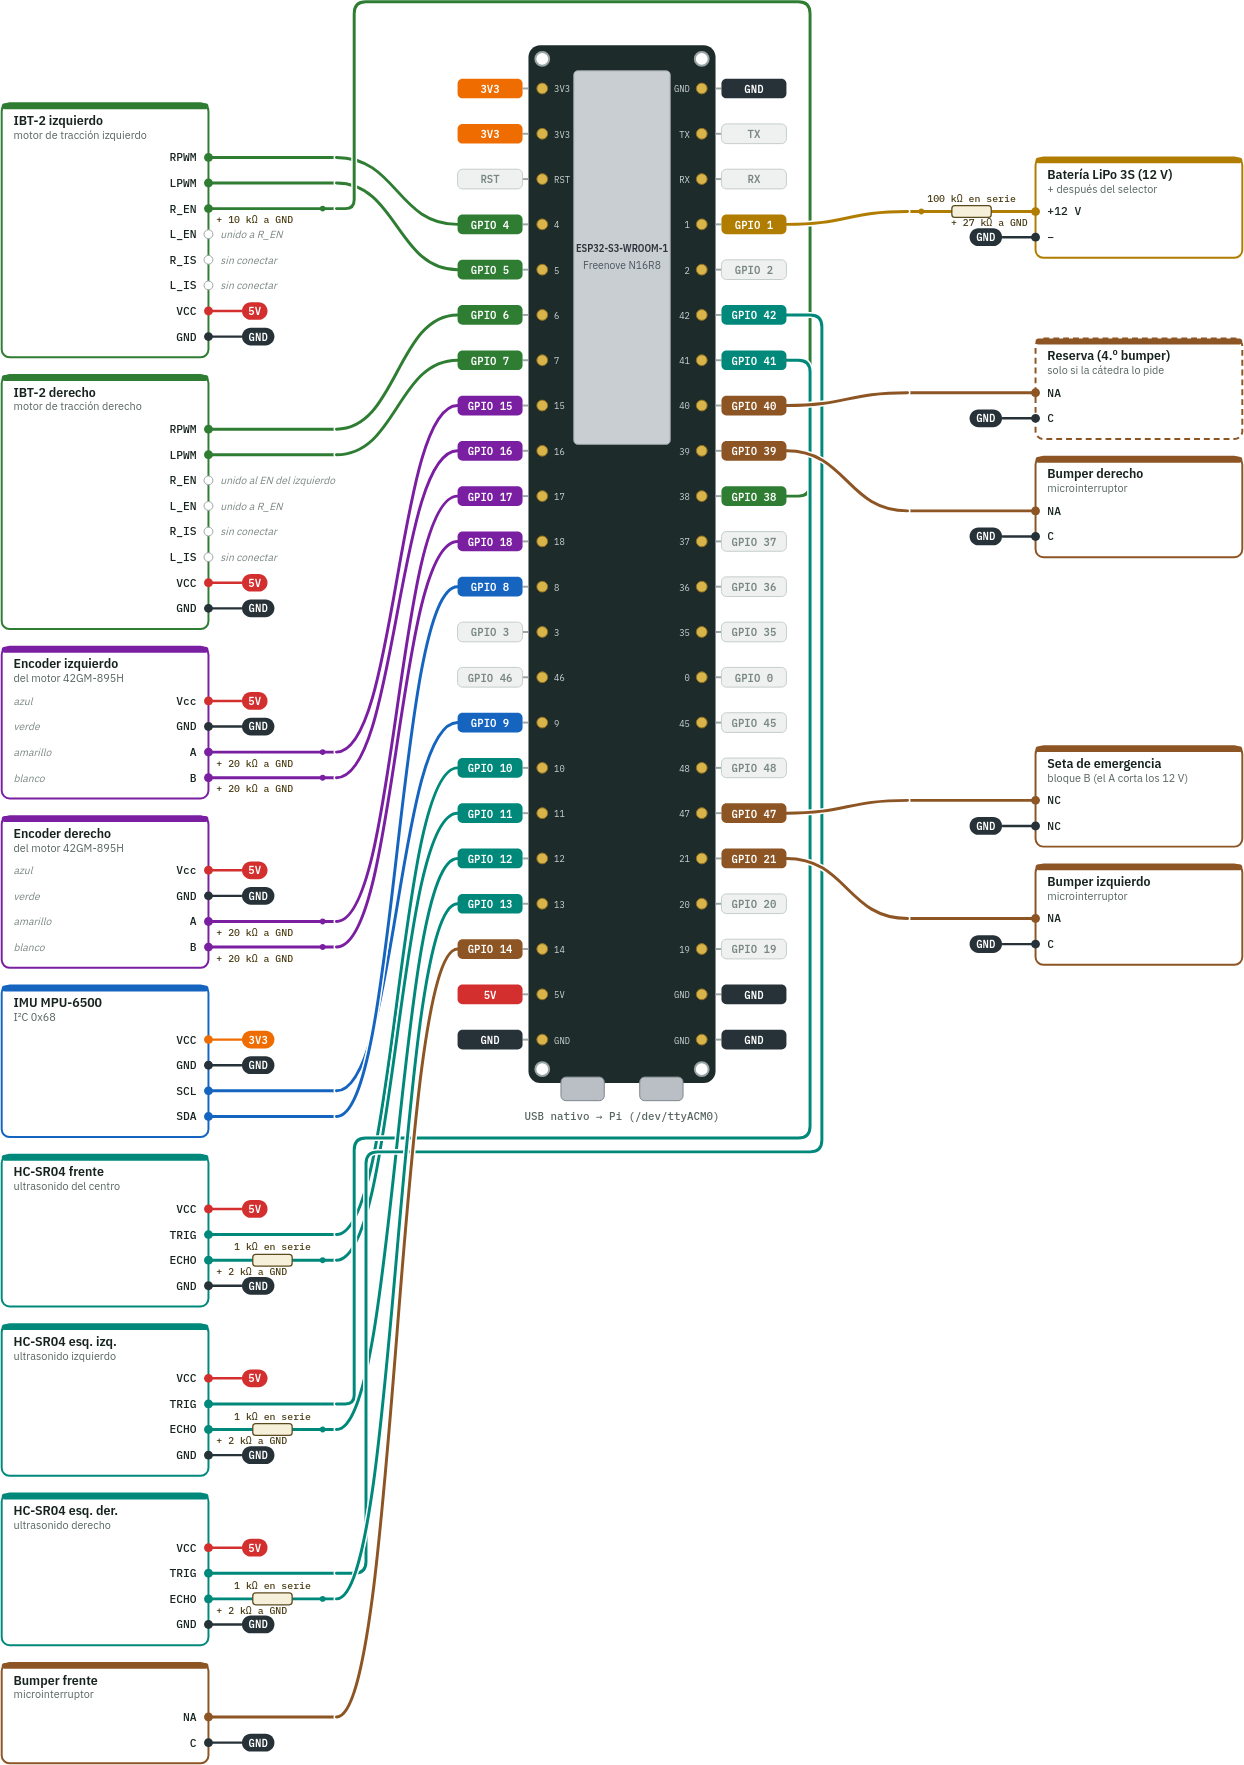
\includegraphics[height=0.82\textheight]{html_s3_cableado.png}
\caption{Cableado de la S3: cada periférico a un costado, con un cable de color de cada pin al pin de la ESP32
(de \archivo{docs/html/placa\_s3.html}). Las resistencias se dibujan sobre el cable.}
\end{figure}

\begin{figure}[H]
\centering
\begin{subfigure}{0.58\textwidth}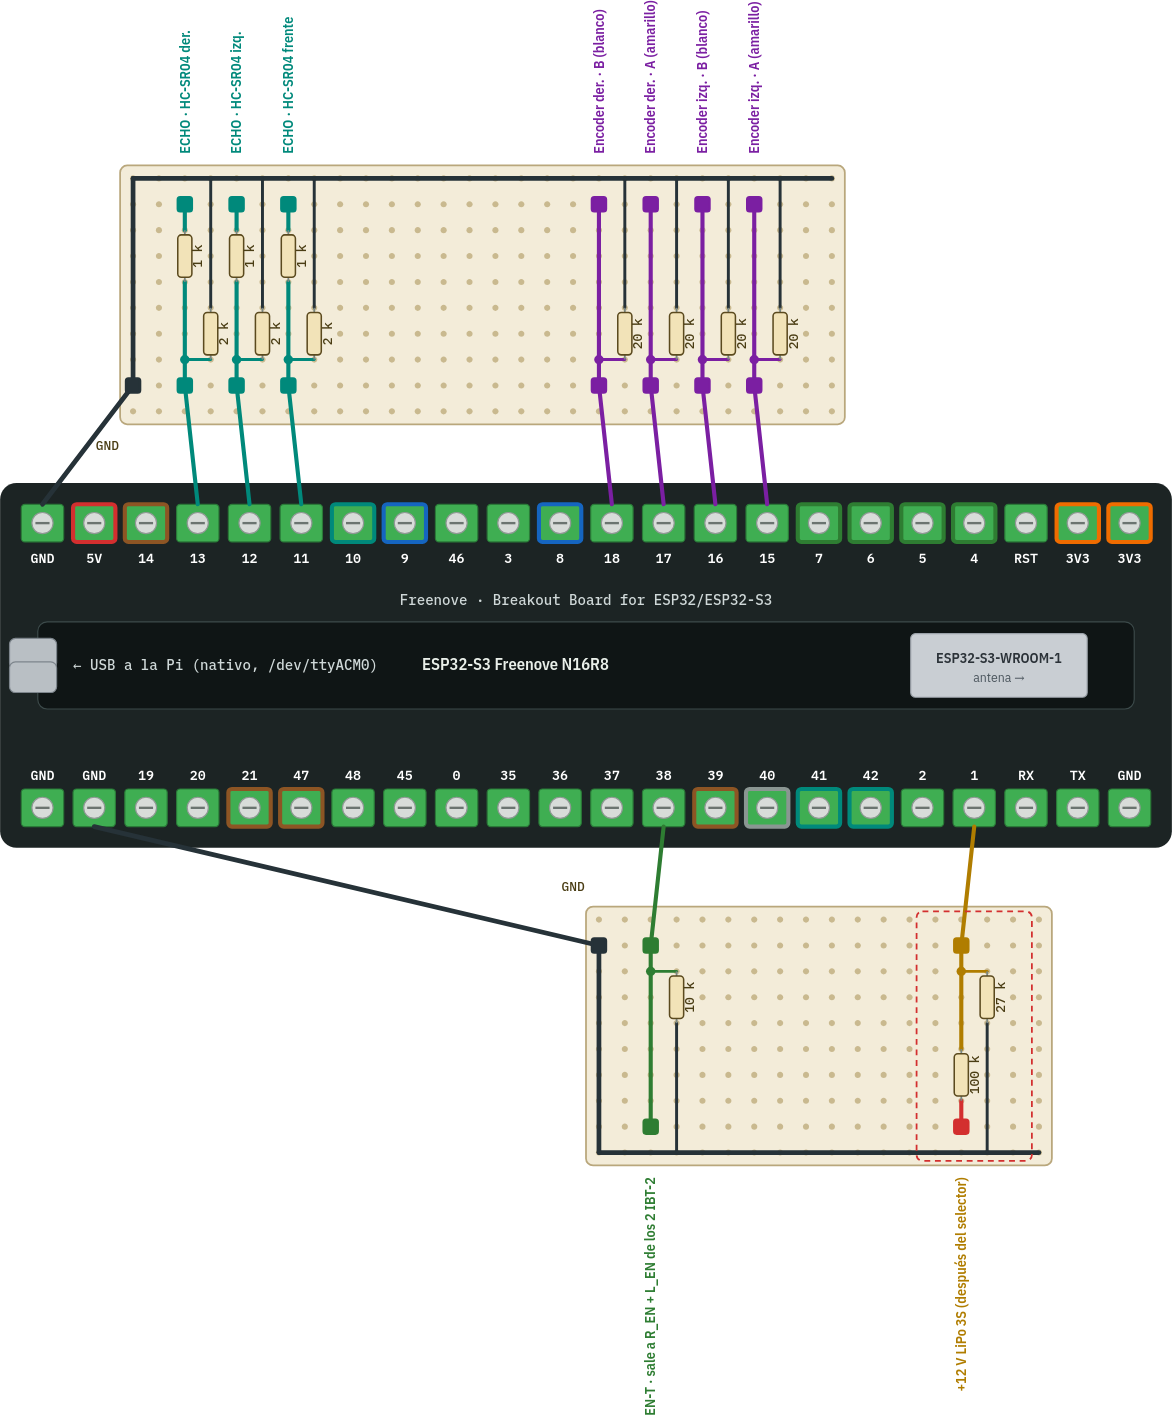
\includegraphics[width=\linewidth]{html_s3_perforadas.png}\caption{La Freenove con las dos perforadas.}\end{subfigure}\hfill
\begin{subfigure}{0.38\textwidth}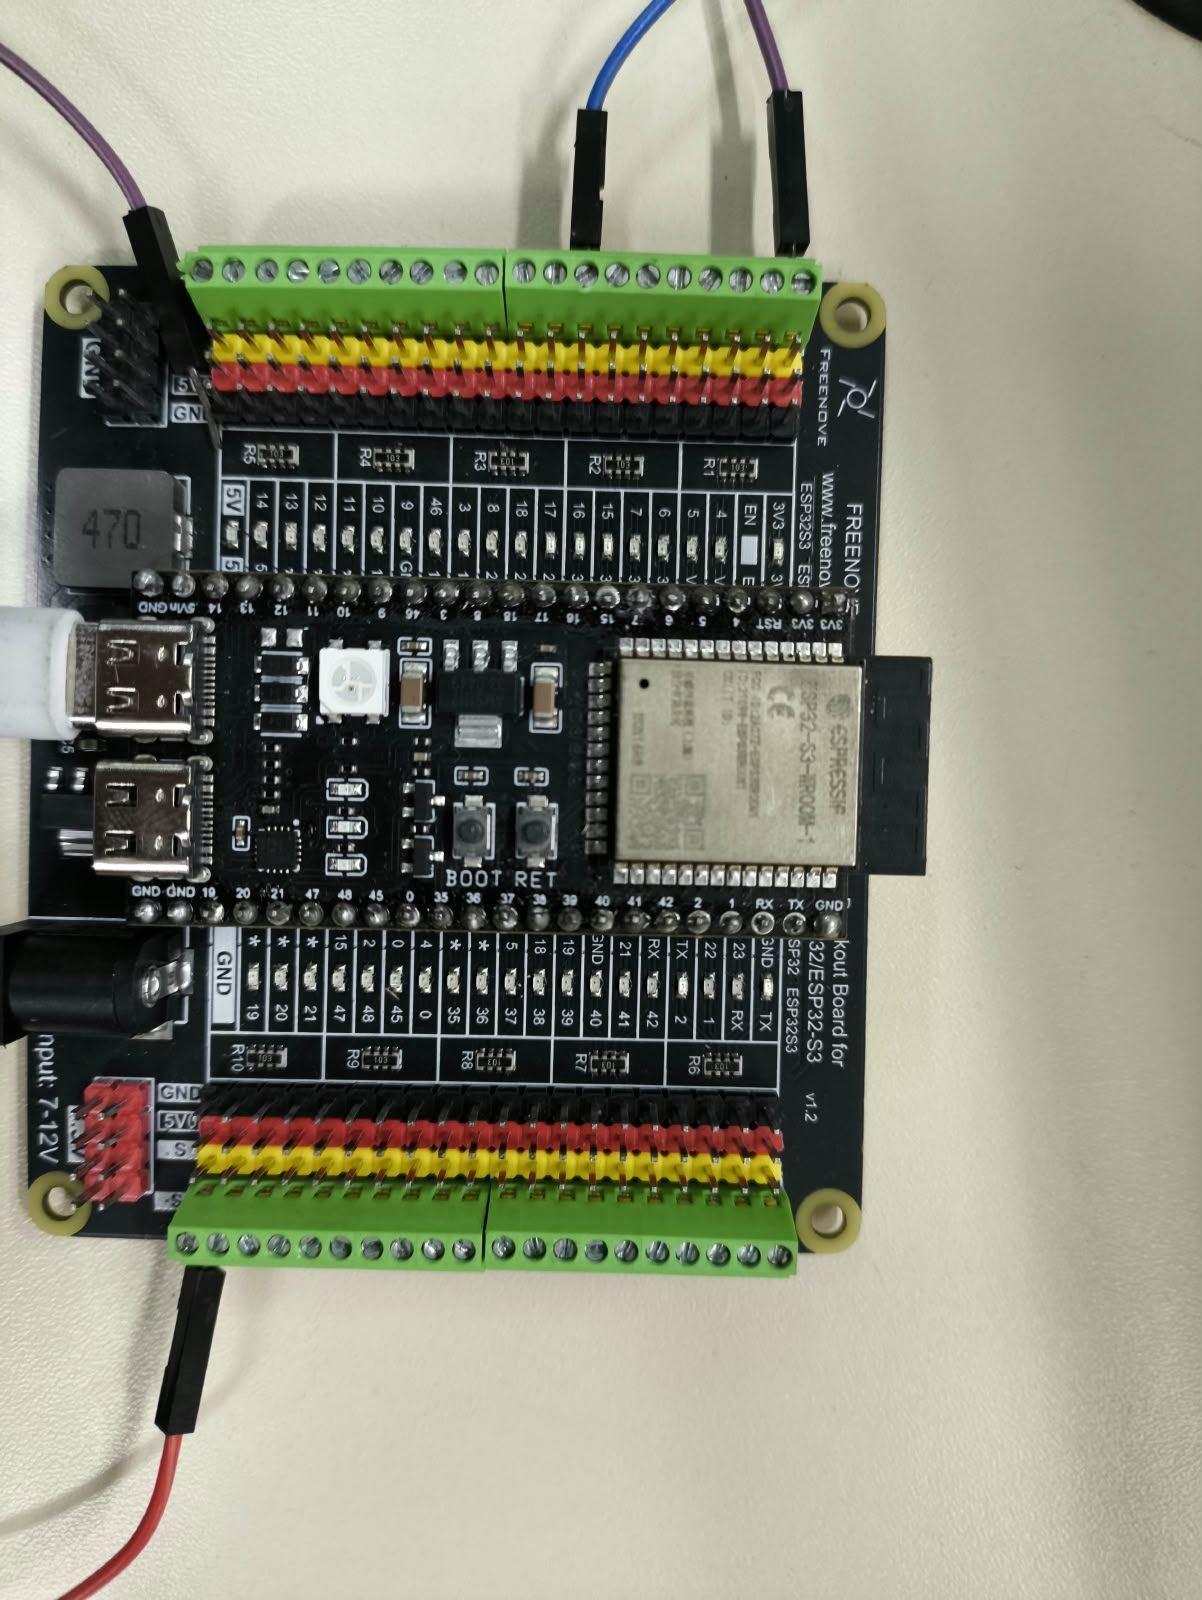
\includegraphics[width=\linewidth]{s3_foto.jpg}\\[4pt]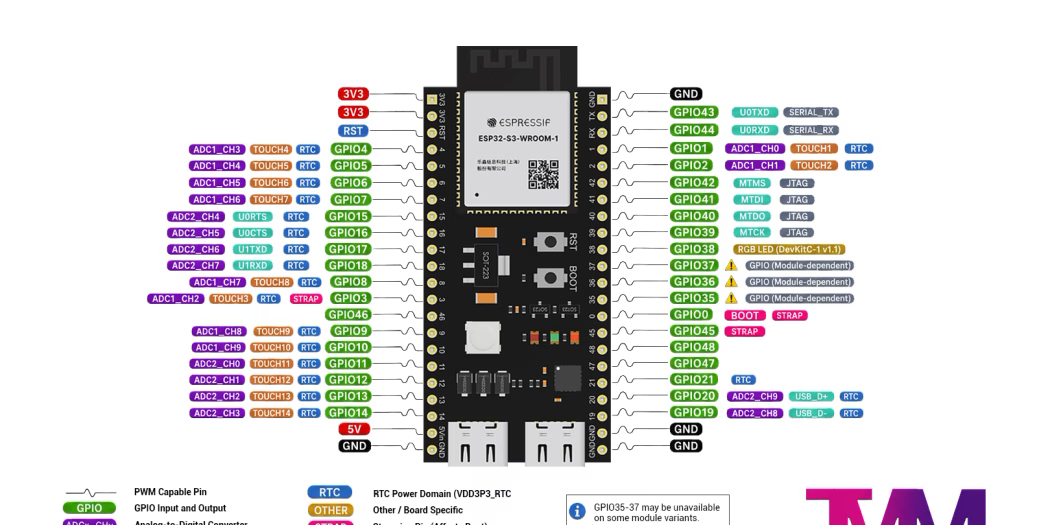
\includegraphics[width=\linewidth]{pinout_s3.png}\caption{Placa real y pinout.}\end{subfigure}
\caption{Montaje de la S3.}
\end{figure}

\section{ESP32-WROOM-32D: el brazo}

Placa HW-394 de 30 pines (USB-C, conversor CH340: aparece como \cod{/dev/ttyUSB0}), enchufada en un \textbf{shield de
borneras}, más una perforada chica de distribución con rieles de 5~V, 3,3~V, EN, GND y 6~V. Pines v0.5 (12/10).

{\small\begin{longtable}{@{}p{2.6cm} p{6.6cm} p{6.4cm}@{}}
\toprule
\textbf{GPIO} & \textbf{Conecta a} & \textbf{Nota} \\
\midrule
\endhead
21 · 22 & J1 IBT-2 RPWM · LPWM & 20~kHz (probado) \\
25 · 26 & J2 IBT-2 RPWM · LPWM & \\
16 · 17 & J3 IBT-2 RPWM · LPWM & \\
23 & R\_EN + L\_EN de los 3 IBT-2 & pull-down 10~kΩ (la única resistencia) \\
34 · 35 & Encoder J1 A · B & solo entrada; pull-up de la placa del encoder \\
36 (VP) · 39 (VN) & Encoder J2 A · B & solo entrada; pull-up de la placa del encoder \\
18 · 19 & Encoder J3 A · B & \\
4 & Servo de apertura & 50~Hz \\
14 & Servo de giro (J4) & saca pulsos al arrancar: el servo puede moverse un instante \\
32 · 33 · 27 & Finales de carrera J1 · J2 · J3 & NA a GND, pull-up interno \\
13 & libre & reserva \\
\bottomrule
\end{longtable}}

Evitar en la WROOM: 6--11 (flash), 0/2/5/12/15 (\textit{strapping}), 1/3 (UART0 = USB).

\begin{nota}[Un solo EN para las tres articulaciones]
Los tres IBT-2 del brazo comparten el EN (GPIO~23). Consecuencia: no se puede dejar una articulación en rueda libre
mientras otra se mueve. La que no se mueve queda \textbf{frenada} (puente habilitado con PWM 0). Rueda libre solo
cuando las tres están libres.
\end{nota}

\begin{figure}[H]
\centering
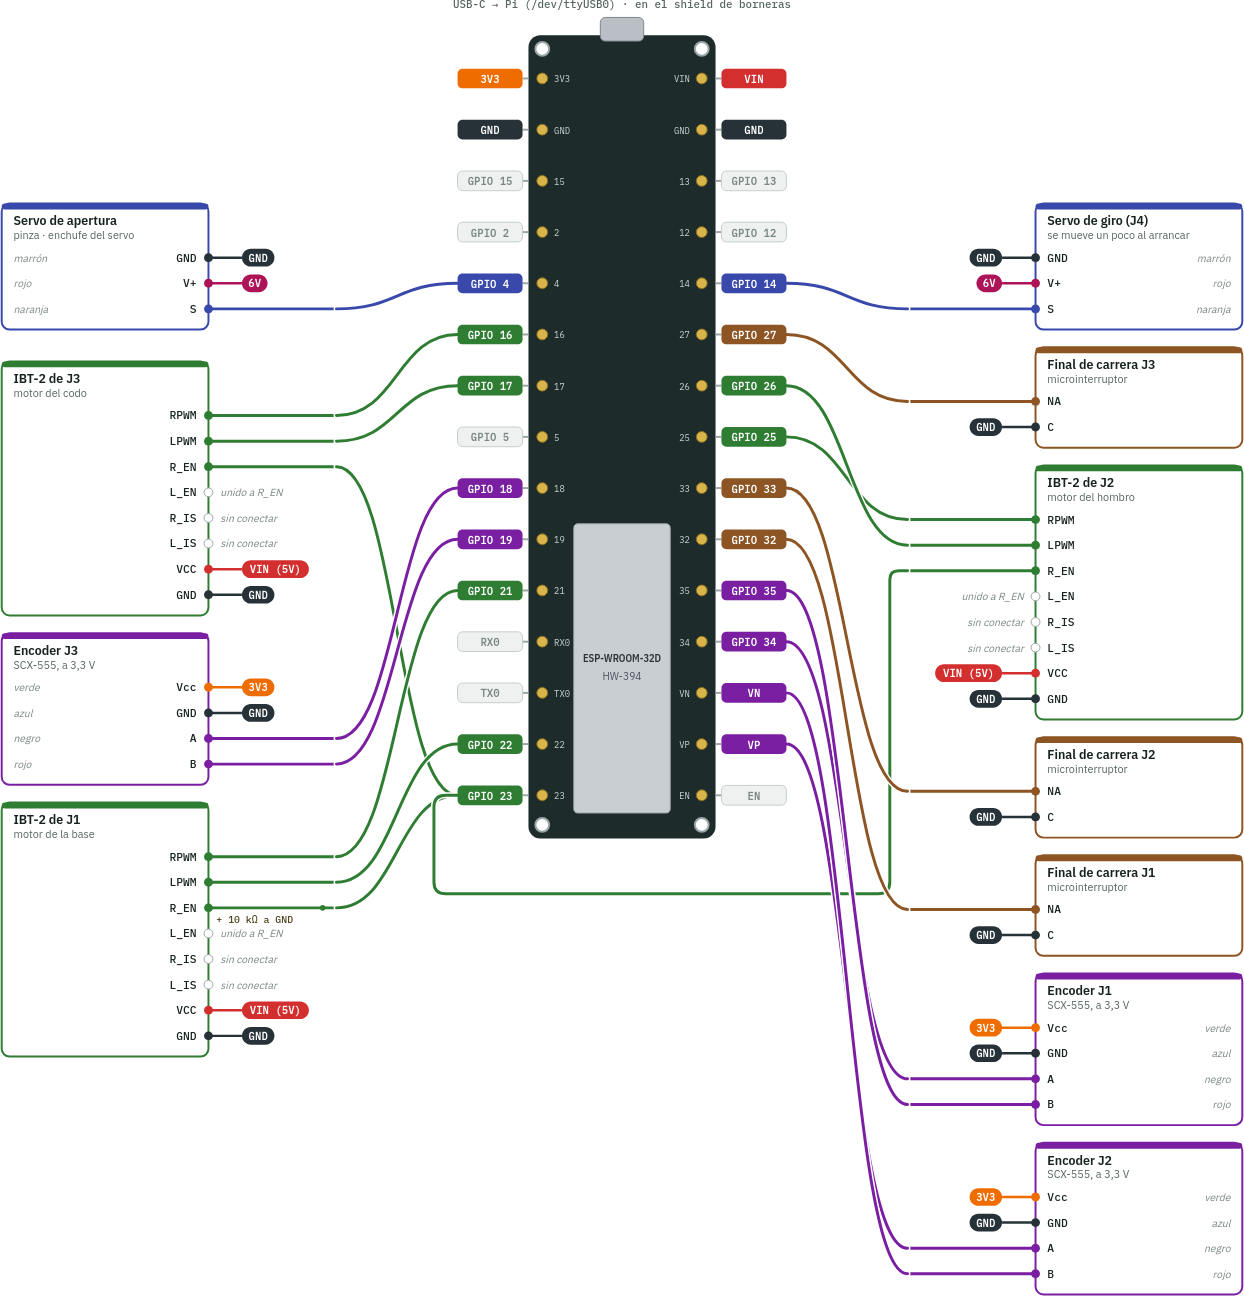
\includegraphics[width=\textwidth]{html_wroom_cableado.png}
\caption{Cableado de la WROOM (de \archivo{docs/html/placa\_wroom.html}).}
\end{figure}

\begin{figure}[H]
\centering
\begin{subfigure}{0.62\textwidth}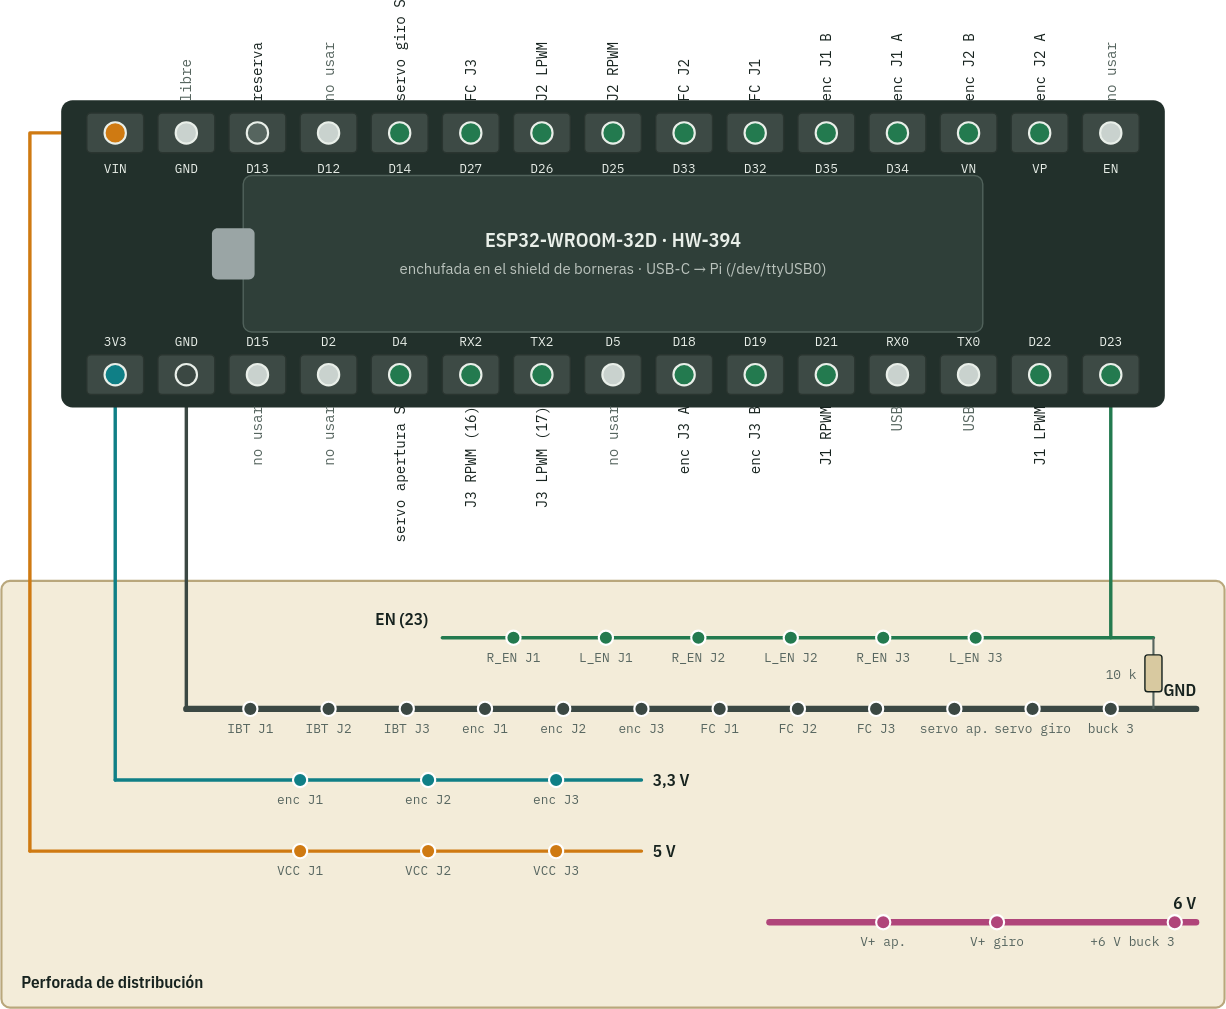
\includegraphics[width=\linewidth]{html_wroom_plano.png}\caption{Shield y perforada de distribución.}\end{subfigure}\hfill
\begin{subfigure}{0.34\textwidth}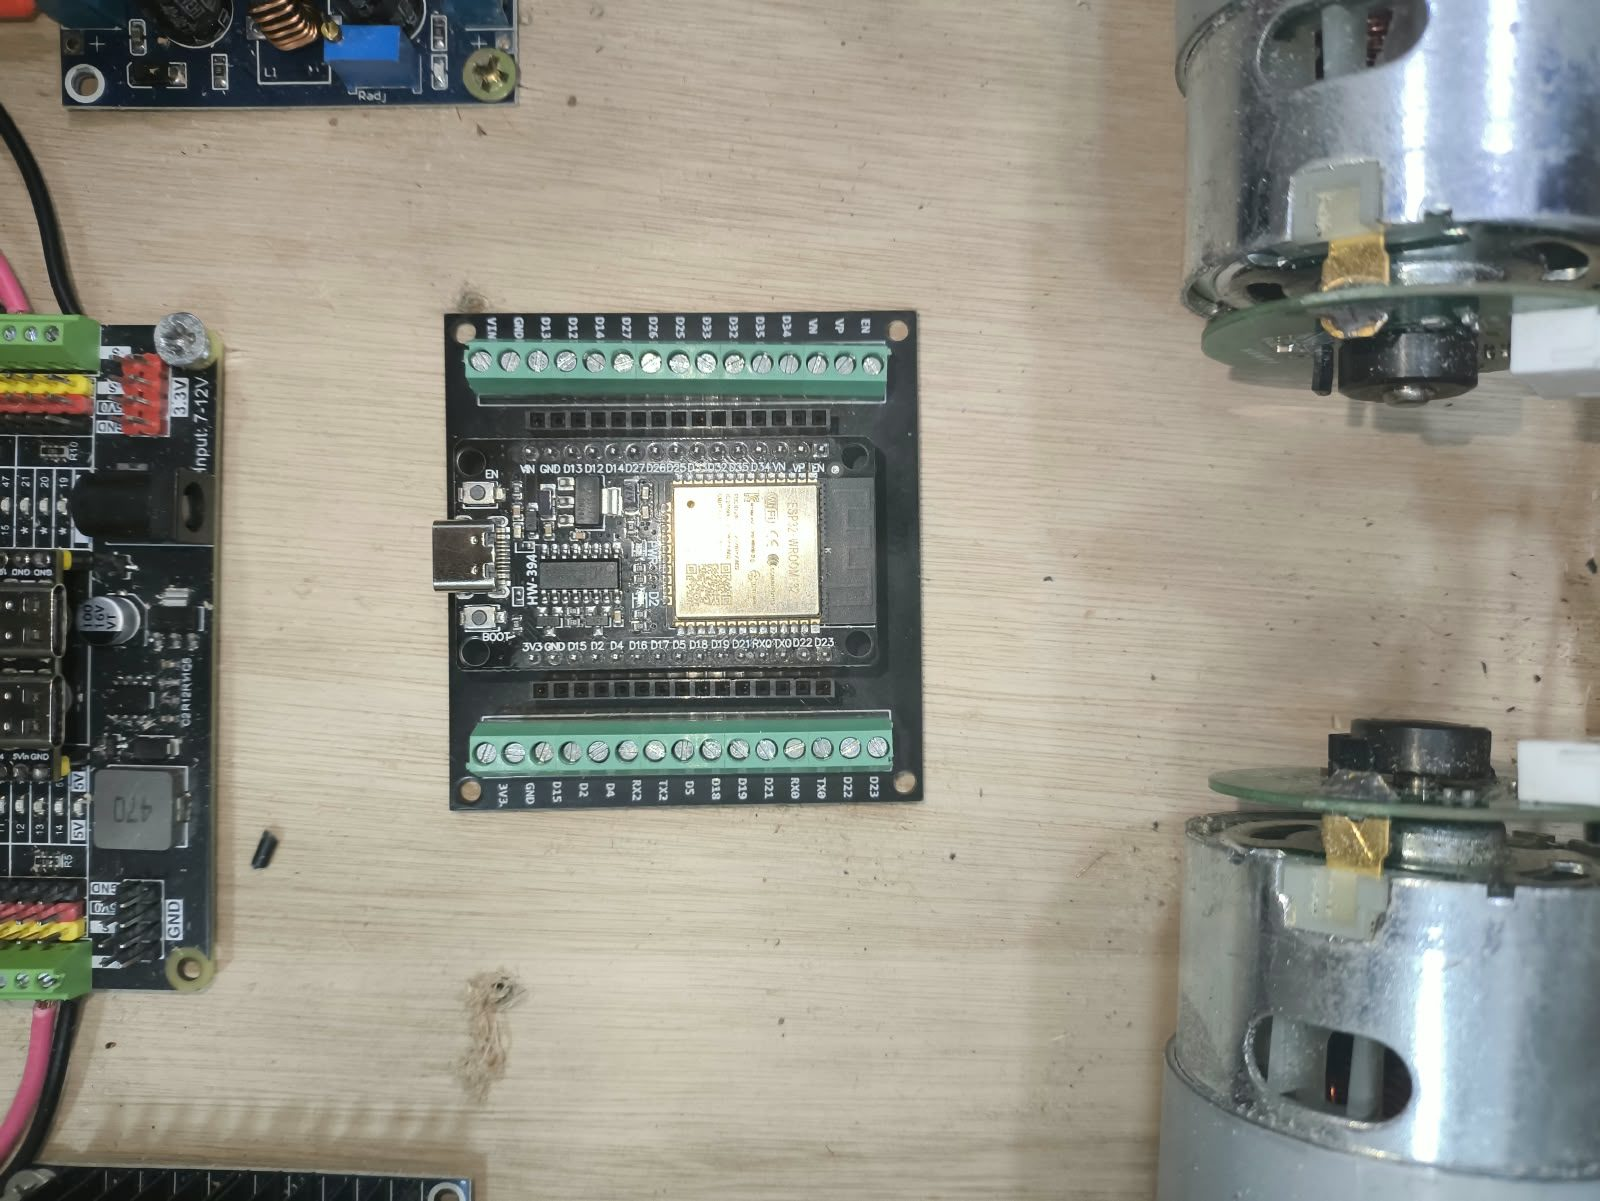
\includegraphics[width=\linewidth]{shield_wroom.jpg}\caption{Shield de borneras real.}\end{subfigure}
\caption{Montaje de la WROOM.}
\end{figure}

\section{Raspberry Pi 5}

{\small
\begin{tabularx}{\textwidth}{@{}l l X@{}}
\toprule
\textbf{Puerto} & \textbf{Conecta a} & \textbf{Nota} \\
\midrule
CSI0 · CSI1 & Cámaras NoIR izquierda · derecha & cable plano de 15 a 22 pines \\
USB & ESP32-S3 (base) & micro-ROS (\cod{/dev/serial/by-id/}\ldots) \\
USB & ESP32-WROOM (brazo) & micro-ROS a 115\,200 baudios \\
GPIO 14 · 15 (pines 8 · 10) & GPS UP501: RX · TX del GPS & UART0, \cod{/dev/ttyAMA0}, 9600 baudios, 3,3~V \\
USB-C & Power bank & 5~V 3~A \\
\bottomrule
\end{tabularx}}

La Pi va \textbf{arriba del mástil, junto a las cámaras}: el cable CSI es corto y sensible a interferencias, mientras
que el USB aguanta 1--2~m. Bajan por el mástil los dos USB hacia los ESP32. Los GPIO se atornillan en un HAT pasivo
de borneras.

\begin{nota}[Por qué usar \cod{/dev/serial/by-id/}]
Los nombres \cod{/dev/ttyACM0} y \cod{/dev/ttyUSB0} pueden cambiar (la S3 pasa a veces de ACM0 a ACM1 al reiniciarse).
Los enlaces de \cod{/dev/serial/by-id/} tienen el nombre del fabricante y no cambian: usarlos en los agentes.
\end{nota}

\begin{nota}[Corriente de los USB]
Sin la fuente oficial de 5~A, la Pi limita a 600~mA el total de los USB \textbf{y el ventilador}. Alcanza para los dos
ESP32 (unos 400~mA con sensores). No activar \cod{usb\_max\_current\_enable=1}. Verificar con la visión corriendo
10~min: \cod{vcgencmd get\_throttled} tiene que dar \cod{0x0}.
\end{nota}

\section{La seta, cable por cable}

\begin{figure}[H]
\centering
\begin{subfigure}{0.40\textwidth}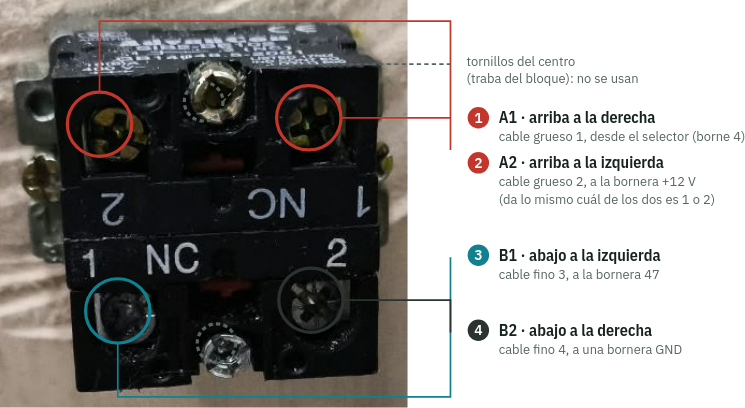
\includegraphics[width=\linewidth]{html_seta_foto.png}\caption{Qué tornillo es cuál.}\end{subfigure}\hfill
\begin{subfigure}{0.56\textwidth}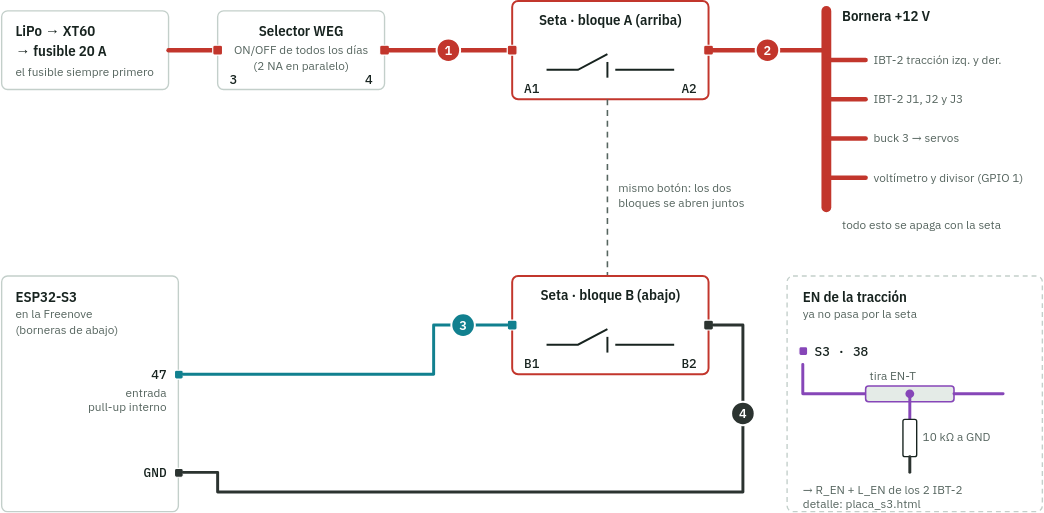
\includegraphics[width=\linewidth]{html_seta_circuito.png}\caption{Los 4 cables.}\end{subfigure}
\caption{La seta (de \archivo{docs/html/seta.html}). Bloque A (arriba): cables 1 y 2, en el + del bus de 12~V.
Bloque B (abajo): cables 3 y 4, entre el GPIO~47 y GND.}
\end{figure}

Antes de cablearla, \textbf{probar con el multímetro qué contactos son NC}. Prueba: con la seta apretada, 0~V en la
bornera +12~V y \cod{armar} tiene que fallar; al soltarla, las ruedas no arrancan solas.

\chapter{Firmware de los ESP32}\label{cap:firmware}

\section{Organización del código}

El firmware está en \archivo{firmware/} y se compila con \textbf{PlatformIO} (\cod{\textasciitilde/.platformio/penv/bin/pio}).
Hay un proyecto por placa y una carpeta de bibliotecas compartidas:

{\small
\begin{tabularx}{\textwidth}{@{}l X@{}}
\toprule
\textbf{Carpeta} & \textbf{Qué tiene} \\
\midrule
\archivo{firmware/lib/ControlArticulacion} & Control de un motor (cascada posición → velocidad), \textbf{sin Arduino} \\
\archivo{firmware/lib/EnlaceMicroRos} & Sesión con el agente: ping, armado, reconexión \\
\archivo{firmware/lib/BTS7960} & Driver del IBT-2 (dos PWM + EN) \\
\archivo{firmware/lib/EncoderPCNT} & Encoder por el contador de pulsos del ESP32 \\
\archivo{firmware/lib/HCSR04} & Los 3 ultrasonidos, sin bloquear (ECHO por interrupción) \\
\archivo{firmware/lib/MPU9250} & IMU (sirve para la MPU-6500) \\
\archivo{firmware/base/} & Proyecto de la S3: \archivo{src/}, \archivo{include/pins.h}, \archivo{include/base\_config.h} \\
\archivo{firmware/base/lib/BaseLogica} & Cinemática diferencial, odometría y seguridad de la base, \textbf{sin Arduino} \\
\archivo{firmware/brazo/} & Proyecto de la WROOM: \archivo{src/}, \archivo{include/pins.h}, \archivo{include/brazo\_config.h} \\
\bottomrule
\end{tabularx}}

Reglas del código:
\begin{itemize}
  \item Los pines están \textbf{solo} en \archivo{include/pins.h}; los parámetros, en \archivo{base\_config.h} o
        \archivo{brazo\_config.h}.
  \item Los drivers compartidos se enlazan con \cod{symlink://../lib/X} (no se copian).
  \item La lógica que no depende de Arduino (control, cinemática, seguridad) se prueba en la PC con
        \cod{pio test -e native}, con un motor simulado con el modelo de la entrega E5.
\end{itemize}

\subsection{Entornos de compilación}
Cada proyecto tiene tres entornos (\archivo{platformio.ini}):
\begin{description}
  \item[\cod{native}] Corre las pruebas en la PC. Base: 20 pruebas. Brazo: 17.
  \item[\cod{esp32s3} / \cod{esp32dev}] Firmware con \textbf{comandos por el monitor serie}. Para probar a mano.
  \item[\cod{ros}] El mismo firmware con \textbf{micro-ROS}: los comandos llegan por tópicos. Es el que se usa con la Pi.
\end{description}

\begin{lstlisting}[language=consola]
PIO=~/.platformio/penv/bin/pio
cd firmware/base                  # o firmware/brazo
$PIO test -e native               # pruebas de la lógica en la PC
$PIO run                          # compilar (modo serial)
$PIO run -t upload -t monitor     # flashear y abrir el monitor (¡12 V APAGADOS!)
$PIO run -e ros -t upload         # flashear la versión micro-ROS (detener antes el agente)
\end{lstlisting}

\section{Cómo corre el programa}

\begin{figure}[H]
\centering
\begin{tikzpicture}[node distance=4mm]
  \node[caja,text width=60mm,align=left] (c0) {\textbf{Núcleo 0: tarea de control (100 Hz)}\\\footnotesize
    cada 10 ms: leer encoders → calcular velocidades → seguridad → control → escribir PWM. Si deja de correr
    1~s, el watchdog de tareas \textbf{reinicia la placa}.};
  \node[caja,text width=60mm,align=left,right=8mm of c0] (c1) {\textbf{Núcleo 1: comunicación}\\\footnotesize
    leer comandos (serie o micro-ROS), validarlos y pasarlos a la tarea de control; publicar estado y sensores.};
  \draw[<->,thick] (c0) -- node[topico,above]{variables}node[topico,below]{protegidas} (c1);
\end{tikzpicture}
\caption{Las dos mitades del firmware. El control nunca espera a la comunicación.}
\end{figure}

\section{El control de un motor: cascada posición → velocidad}

La entrega E5 identificó cada motor como un \textbf{sistema de primer orden} de duty (\%) a velocidad (rpm):
\[
G(s) = \frac{\omega(s)}{u(s)} = \frac{K}{\tau s + 1}
\qquad\text{(J1: } K = 1{,}58~\text{rpm}/\%,\ \tau = 0{,}065\text{ s)}
\]
Como el modelo es de \textbf{velocidad}, el control es en \textbf{cascada}: un lazo externo de posición genera la
velocidad que tiene que seguir un lazo interno de velocidad.

\begin{figure}[H]
\centering
\resizebox{\textwidth}{!}{%
\begin{tikzpicture}[node distance=9mm,every node/.style={font=\small}]
  \node (qref) {$q_\text{obj}$};
  \node[circle,draw,right=6mm of qref,inner sep=1pt] (s1) {$\Sigma$};
  \node[caja,right=of s1] (pp) {P posición\\$K_{pp}\,e_q$};
  \node[caja,right=of pp] (sat) {saturación\\$v_\text{máx}$, $a_\text{máx}$};
  \node[circle,draw,right=of sat,inner sep=1pt] (s2) {$\Sigma$};
  \node[caja,right=of s2] (pi) {PI velocidad\\+ anti-windup};
  \node[circle,draw,right=of pi,inner sep=1pt] (s3) {$+$};
  \node[caja,above=7mm of s3] (ff) {feedforward\\zona muerta $u_0$ (+ $\omega/K$)};
  \node[caja,right=of s3] (ibt) {límite\\duty};
  \node[caja,right=of ibt] (mot) {IBT-2 +\\motor $\frac{K}{\tau s+1}$};
  \node[right=7mm of mot] (q) {$q$};
  \node[caja,below=9mm of pi] (enc) {encoder (PCNT)\\cuentas → $q$, $\omega$};
  \draw[->] (qref) -- (s1); \draw[->] (s1) -- node[above]{$e_q$} (pp); \draw[->] (pp) -- (sat);
  \draw[->] (sat) -- node[above]{$\omega_\text{ref}$} (s2); \draw[->] (s2) -- node[above]{$e_\omega$} (pi);
  \draw[->] (pi) -- (s3); \draw[->] (ff) -- (s3); \draw[->] (s3) -- (ibt); \draw[->] (ibt) -- node[above]{$u$ [\%]} (mot);
  \draw[->] (mot) -- (q);
  \draw[->] (mot.south) |- (enc);
  \draw[->] (enc.west) -| node[pos=0.8,left]{$\omega$} (s2.south);
  \draw[->] ($(enc.west)+(0,-0.2)$) -| node[pos=0.85,left]{$q$} (s1.south);
  \draw[->,gris] (sat.north) |- (ff.west);
  \node[font=\scriptsize,gris,anchor=north west] at ($(qref.south)+(-0.2,-1.6)$) {lazo externo (solo brazo)};
\end{tikzpicture}}
\caption{Control en cascada de \archivo{ControlArticulacion}. Las ruedas usan solo el lazo interno (velocidad).}
\label{fig:cascada}
\end{figure}

Lo que hace la tarea de control en cada paso (10~ms), para una articulación del brazo:

\begin{enumerate}
  \item \textbf{Error de posición}: $e_q = q_\text{obj} - q$.
  \item \textbf{Llegada con histéresis}: si $|e_q| < $ tolerancia (0,3° en J1), se considera que llegó y el motor
        queda frenado; recién se vuelve a mover si el error supera el doble (0,6°). Así no ``tiembla'' alrededor
        del objetivo.
  \item \textbf{Velocidad deseada}: $\omega_\text{des} = K_{pp}\, e_q$, saturada a $v_\text{máx}$ (30~°/s en J1) y con
        un mínimo $v_\text{mín}$ (3~°/s) para que no se clave a 1° del objetivo.
  \item \textbf{Rampa}: $\omega_\text{ref}$ se acerca a $\omega_\text{des}$ cambiando como mucho $a_\text{máx}\,\Delta t$
        (60~°/s²). El resultado es un perfil de velocidad aproximadamente \textbf{trapezoidal}.
  \item \textbf{Lazo de velocidad}: $e_\omega = \omega_\text{ref} - \omega$, y
        \[
          u = \underbrace{\operatorname{sgn}\cdot u_0 + \tfrac{\omega_\text{ref}}{K}}_{\text{feedforward}}
              + K_p\, e_\omega + K_i \!\int\! e_\omega\, dt
        \]
        donde $u_0$ es la \textbf{zona muerta} (el duty mínimo para que el motor arranque: 17~\% en J1). En J1 se usa
        solo la zona muerta como feedforward (\cod{ffSoloZonaMuerta}).
  \item \textbf{Anti-windup condicional}: si $u$ ya está saturado en el sentido del error, el integrador no acumula.
  \item \textbf{Límite de duty}: 40~\% en la puesta en marcha.
\end{enumerate}

\subsection{Parámetros de J1 (medidos el 02/10)}
\begin{center}
\begin{tabular}{@{}lll@{}}
\toprule
\textbf{Parámetro} & \textbf{Valor} & \textbf{Significado} \\
\midrule
Cuentas por vuelta del motor & 3200 & 16 PPR × 4 × 50 \\
Relación de la correa & 5 & 18 → 90 dientes \\
Rango & 45° a 225° & marco de \cod{brazo\_ik} \\
Modelo & $K = 1{,}58$, $\tau = 0{,}065$~s & E5 \\
Zona muerta & 17~\% & medida con el brazo \\
PI de velocidad & $K_p = 0{,}659$~\%/rpm, $K_i = 4{,}8$ & \\
$K_{pp}$, $v_\text{máx}$, $a_\text{máx}$ & 2~1/s, 30~°/s, 60~°/s² & \\
Tolerancia de llegada & 0,3° & \\
Atasco & duty $\geq$ 35~\% y $<$ 1,7~rpm durante 0,3~s & → falla \\
Signos & \cod{ENC\_INVERTIDO} y \cod{MOTOR\_INVERTIDO} en \cod{true} & \\
\bottomrule
\end{tabular}
\end{center}

\begin{pendiente}
J2 y J3 arrancan con los parámetros de J1 llevados a 58~rpm ($K \times 58/160$; $K_p$ y $K_i \times 160/58$). Hay que
medirlos con los motores nuevos: signos, zona muerta, $K$, $\tau$ y PI (pasos 0--3 de \archivo{pruebas-esp32/10}).
\end{pendiente}

\section{Firmware de la base (S3)}

\subsection{Velocidad de las ruedas}
\topic{/cmd\_vel} trae $(v, \omega)$. La S3 aplica la rampa, calcula las rpm de cada rueda con la cinemática
diferencial (figura~\ref{fig:diferencial}) y cada rueda tiene su propio lazo PI de velocidad (el mismo
\archivo{ControlArticulacion}, en modo velocidad). Si una rueda falla, las dos se frenan en el mismo paso.

\subsection{Odometría}
Con las cuentas de los encoders, cada 10~ms se calcula cuánto avanzó cada rueda ($\Delta s_i$, $\Delta s_d$) y se
integra la pose $(x, y, \theta)$ en el marco \cod{odom}:
\[
\Delta s = \frac{\Delta s_d + \Delta s_i}{2}, \quad
\Delta\theta = \frac{\Delta s_d - \Delta s_i}{b}, \quad
x \mathrel{+}= \Delta s \cos\!\left(\theta + \tfrac{\Delta\theta}{2}\right), \quad
y \mathrel{+}= \Delta s \sin\!\left(\theta + \tfrac{\Delta\theta}{2}\right), \quad
\theta \mathrel{+}= \Delta\theta
\]
Se publica en \topic{/odom} a 25~Hz. Es buena para distancias cortas en línea recta; en giros cerrados las ruedas
patinan y el ángulo se desvía. Por eso el recorrido autónomo toma el \textbf{rumbo del giróscopo} y solo el
\textbf{avance} de las ruedas (capítulo~\ref{cap:mision}).

\subsection{Seguridad de la base}
Se decide en la S3, sin esperar a la Pi:

\begin{longtable}{@{}p{5.2cm} p{5.6cm} p{4.4cm}@{}}
\toprule
\textbf{Causa} & \textbf{Qué hace} & \textbf{Cómo se sale} \\
\midrule
\endhead
Seta apretada (o cable cortado) & EMERGENCIA: puentes deshabilitados (EN = 0) & Soltar la seta, \cod{r} y \cod{armar} \\
Inclinación (roll o pitch) $> 25^\circ$ & VUELCO: frena & Nivelar la base y \cod{r} \\
IMU sin muestras por más de 200~ms & No se mueve (no puede vigilar el vuelco) & Solo, al volver los datos \\
Bumper del frente & No avanza; solo puede alejarse en línea recta & Solo, al soltarse \\
Bumper lateral & No gira (el costado barrería el objeto) & Solo, al soltarse \\
Ultrasonido del frente sin eco & No avanza; retroceder y girar sí & Solo, al volver el eco \\
Obstáculo al frente $< 0{,}20$~m & No avanza & Solo \\
Obstáculo entre 0,20 y 0,50~m & Tope de velocidad que baja linealmente a 0 & Solo \\
Sin \topic{/cmd\_vel} por 300~ms & Frena y anula el comando vigente & Con un comando nuevo \\
Batería $<$ 10,5~V & Aviso \cod{BATERIA\_BAJA} (no frena) & — \\
Rueda atascada o encoder con saltos & Base detenida & \cod{r} \\
\bottomrule
\end{longtable}

\begin{figure}[H]
\centering
\begin{tikzpicture}[scale=1]
  \fill[verde!20] (0,0) rectangle (2,2.5);
  \fill[naranja!25] (2,0) -- (2,2.5) -- (5,2.5) -- cycle;
  \fill[rojo!15] (0,0) rectangle (2,0.02);
  \draw[->] (0,0) -- (6,0) node[right]{distancia al frente [m]};
  \draw[->] (0,0) -- (0,3) node[above]{velocidad máxima de avance};
  \draw[very thick,rojo] (0,0) -- (2,0);
  \draw[very thick,acento] (2,0) -- (5,2.5) -- (5.8,2.5);
  \node[below] at (2,0) {0,20}; \node[below] at (5,0) {0,50};
  \node[left] at (0,2.5) {0,25 m/s};
  \node[font=\small,rojo] at (1,0.4) {no avanza};
  \node[font=\small,acento,rotate=40] at (3.3,1.5) {tope lineal};
\end{tikzpicture}
\caption{Tope de velocidad por cercanía de un obstáculo (HC-SR04 del frente). Retroceder y girar siempre se permite.}
\end{figure}

\subsection{Comandos por el monitor serie (base)}
\begin{longtable}{@{}p{3.6cm} p{11.9cm}@{}}
\toprule
\textbf{Comando} & \textbf{Qué hace} \\
\midrule
\endhead
\cod{e} & Estado: modo, seguridad, odometría y ruedas \\
\cod{sens} & Sensores: IMU, distancias, bumpers, seta, batería \\
\cod{v <v> <w> [s]} & Mover con rampa (m/s, rad/s) por \cod{s} segundos (por defecto 1, máximo 3). Ej.: \cod{v 0.1 0} \\
\cod{w <izq> <der> [s]} & rpm de cada rueda (solo el lazo de velocidad). Ej.: \cod{w 20 20} \\
\cod{d <izq> <der>} & Lazo abierto en \% (máximo 40); se corta a los 300~ms si no se repite \\
\cod{s} & Detener (freno) \\
\cod{l} & Liberar: puentes deshabilitados (rueda libre) \\
\cod{r} & Rearmar tras seta o vuelco (con la causa despejada) y borrar fallas \\
\cod{cal} & Calibrar el giróscopo (robot quieto, 2~s) \\
\cod{odo0} & Odometría a cero \\
\cod{log [hz]} & CSV para graficar (t, v, w, rpm de referencia y medidas, duty, x, y, θ); \cod{log 0} apaga \\
\cod{wd <ms>} & Watchdog de comandos (0 = apagado; con la Pi, 300) \\
\cod{?} & Ayuda \\
\bottomrule
\end{longtable}

\section{Firmware del brazo (WROOM)}

\subsection{El cero y el homing}
El encoder solo cuenta \textbf{cuánto se movió}, no dónde está. Al encender, el firmware no sabe el ángulo de cada
articulación y \textbf{rechaza todo movimiento en posición} hasta tener un cero. Hay dos formas:

\begin{description}
  \item[Cero manual (\cod{z})] Se lleva el brazo a mano (o con \cod{d}) a la pose de referencia
        (\cod{POSE\_CERO} = 90°, 90°, 0°) y se manda \cod{z}: ``el brazo \textbf{está} en esa pose''.
  \item[Homing (\cod{home <n>})] La articulación \cod{n} va despacio (10~rpm del motor) hacia su final de carrera.
        Cuando lo toca (3 lecturas seguidas en bajo), fija su ángulo en \cod{HOME\_Q} (\textbf{MEDIR}). De a una
        articulación. Se cancela si se pasa del recorrido máximo (rango + 10°), del tiempo (25~s) o si aparece una
        falla. Rechaza empezar con el final de carrera ya apretado.
\end{description}

\subsection{Protecciones del brazo}
\begin{itemize}
  \item Sin cero, no acepta movimientos en posición.
  \item Los objetivos se recortan a los límites de la E4. Fuera de los límites + 5° → falla y freno.
  \item Atasco (duty alto sin avanzar) → falla y freno. También detecta un encoder desconectado.
  \item Lecturas imposibles del encoder se descartan; 5 seguidas → falla.
  \item \cod{s}, el fin de \cod{d}/\cod{v} y el watchdog \textbf{frenan hasta que el eje queda quieto} y recién ahí
        sostienen la posición (no vuelven hacia atrás por la inercia).
  \item \cod{d} limitado a 30~\% y se corta a los 300~ms si no se repite; \cod{v} hasta 30~rpm y 5~s.
  \item Los servos no reciben pulsos hasta el primer \cod{pinza}/\cod{giro}.
  \item Watchdog de tareas: si la tarea de control se cuelga 1~s, la placa se reinicia.
\end{itemize}

\subsection{Comandos por el monitor serie (brazo)}
\begin{longtable}{@{}p{3.6cm} p{11.9cm}@{}}
\toprule
\textbf{Comando} & \textbf{Qué hace} \\
\midrule
\endhead
\cod{e} & Estado de las articulaciones \\
\cod{z [n]} & Cero manual: el brazo está en la pose de referencia (todas o la \cod{n}) \\
\cod{home <n>} & Homing con final de carrera de la articulación \cod{n} \\
\cod{m <q1> <q2> <q3>} & Mover las tres (grados). Ej.: \cod{m 90 90 0} \\
\cod{j <n> <q>} & Mover una articulación. Ej.: \cod{j 2 45} \\
\cod{v <n> <rpm> [s]} & Solo el lazo de velocidad (rpm del motor, máx. 30) por \cod{s} segundos \\
\cod{d <n> <pct>} & Lazo abierto (máx. 30~\%); se corta a los 300~ms si no se repite \\
\cod{s} & Detener: frena y, ya quieto, sostiene la posición \\
\cod{l} & Liberar: puentes deshabilitados (rueda libre: \textbf{J2 y J3 caen}) \\
\cod{r} & Borrar fallas (queda detenido) \\
\cod{pinza <0-100>} & 0 = abierta, 100 = cerrada \\
\cod{giro <grados>} & Giro de la pinza (J4), $-90$ a $90$ \\
\cod{log <n> [hz]} & CSV de la articulación \cod{n} (t, q objetivo, q, ω ref, ω, duty) \\
\cod{wd <ms>} & Watchdog de comandos \\
\cod{?} & Ayuda \\
\bottomrule
\end{longtable}

Con micro-ROS, \textbf{los mismos comandos} se mandan como texto por \topic{/base/comando} o \topic{/brazo/comando},
con las mismas validaciones (capítulo~\ref{cap:microros}).

\chapter{ROS 2 desde cero}\label{cap:ros2}

Este capítulo explica ROS~2 con los ejemplos del propio robot. Al terminarlo se puede mirar qué pasa dentro del
robot, mandarle órdenes a mano y escribir un nodo propio.

\section{Los conceptos}

\subsection{Nodos, tópicos y mensajes}

\begin{figure}[H]
\centering
\begin{tikzpicture}[node distance=10mm and 18mm]
  \node[nodo] (tel) {\cod{teleop\_twist\_keyboard}\\(publica)};
  \node[draw=acento,thick,fill=white,rounded corners=10pt,right=of tel,font=\ttfamily\small] (top) {/cmd\_vel};
  \node[nodo,right=of top] (base) {ESP32-S3 (micro-ROS)\\(suscribe)};
  \node[nodo,below=of top] (bag) {\cod{ros2 bag record}\\(también suscribe)};
  \draw[datos] (tel) -- node[topico,above]{Twist} (top);
  \draw[datos] (top) -- node[topico,above]{Twist} (base);
  \draw[datos] (top) -- (bag);
  \node[font=\scriptsize,gris,below=1mm of top,xshift=22mm] {tipo: \cod{geometry\_msgs/msg/Twist}};
\end{tikzpicture}
\caption{Un tópico es un canal con nombre. Quien publica no sabe quién escucha, y puede haber varios de cada lado.}
\end{figure}

\begin{description}
  \item[Nodo] Un programa que participa del sistema: \cod{brazo\_ik}, \cod{mision}, el detector YOLO, cada ESP32.
  \item[Tópico] Un canal con nombre, como \topic{/cmd\_vel}. Cualquier nodo puede publicar en él o suscribirse.
  \item[Mensaje] Lo que viaja por el tópico. Tiene un \textbf{tipo fijo} con campos definidos. Por ejemplo
        \cod{geometry\_msgs/msg/Twist} tiene \cod{linear} (x, y, z) y \cod{angular} (x, y, z). En \topic{/cmd\_vel}
        solo se usan \cod{linear.x} (avance, m/s) y \cod{angular.z} (giro, rad/s).
  \item[Publicar / suscribir] Mandar mensajes / recibirlos. Es asincrónico: el que publica no espera respuesta.
\end{description}

\subsection{Otras piezas}
\begin{description}
  \item[Parámetros] Valores de configuración de un nodo (\cod{largo\_herramienta}, \cod{marco}\ldots). Se pasan al
        arrancar (\cod{--ros-args -p nombre:=valor}) o desde un \textit{launch}.
  \item[Launch] Un archivo Python que arranca varios nodos con sus parámetros de una vez
        (\archivo{mision.launch.py}, \archivo{sim.launch.py}, \archivo{limon.launch.py}).
  \item[TF] Árbol de marcos de coordenadas. Cada mensaje con posición dice en qué marco está (\cod{header.frame\_id}),
        y TF sabe convertir de un marco a otro. Ej.: el limón llega en \cod{camera} y el brazo lo necesita en
        \cod{brazo\_base}.
  \item[Paquete] Carpeta con nodos, \textit{launch} y pruebas, que se compila con \cod{colcon}. En este repo:
        \cod{brazo\_ik}, \cod{mision}, \cod{simulacion} (en \archivo{ros2\_ws/src/}); en el repo de visión,
        \cod{yolo\_ros}.
  \item[Workspace] Carpeta con un \archivo{src/} de paquetes. \cod{colcon build} crea \archivo{build/},
        \archivo{install/} y \archivo{log/}.
  \item[Descubrimiento (DDS)] Los nodos se encuentran solos por la red local. Todos los que estén en la misma LAN y el
        mismo \cod{ROS\_DOMAIN\_ID} (0 por defecto) se ven entre sí.
\end{description}

\begin{peligro}[Cualquier computadora de la red puede mover el robot]
Una notebook con ROS~2 en la misma red Wi-Fi que la Pi ve los tópicos de los ESP32 reales y los puede comandar. La
simulación se aísla con \cod{export ROS\_AUTOMATIC\_DISCOVERY\_RANGE=LOCALHOST} en cada terminal (el \textit{launch}
de la simulación ya lo pone). Con el robot real, no dejar nodos corriendo con el brazo armado si no se usan.
\end{peligro}

\section{Preparar una terminal}

Cada terminal nueva necesita ``cargar'' ROS~2 y los workspaces que se vayan a usar:

\begin{lstlisting}[language=consola]
source /opt/ros/jazzy/setup.bash                    # ROS 2 base (siempre)
source ~/microros_ws/install/local_setup.bash       # para correr el agente micro-ROS (en la Pi)
source ~/recolector_de_frutas/ros2_ws/install/setup.bash   # brazo_ik, mision, simulacion
source ~/yolo_ws/install/setup.bash                 # yolo_ros (visión, en la Pi)
\end{lstlisting}

Compilar los paquetes del robot (después de cambiar algo):

\begin{lstlisting}[language=consola]
cd ~/recolector_de_frutas/ros2_ws
source /opt/ros/jazzy/setup.bash
colcon build --symlink-install            # --symlink-install: los .py se enlazan, no hace falta recompilar al editarlos
source install/setup.bash
colcon test && colcon test-result --verbose   # correr las pruebas
\end{lstlisting}

Conectarse a la Pi:
\begin{lstlisting}[language=consola]
ssh r2d2@100.116.96.71          # por Tailscale (desde cualquier red); en la LAN del lab: 192.168.2.219
\end{lstlisting}

\section{Mirar qué está pasando}

\begin{longtable}{@{}p{7.2cm} p{8.3cm}@{}}
\toprule
\textbf{Comando} & \textbf{Para qué} \\
\midrule
\endhead
\cod{ros2 node list} & Qué nodos están corriendo \\
\cod{ros2 topic list -t} & Qué tópicos existen y de qué tipo \\
\cod{ros2 topic echo /base/estado --field data} & Ver los mensajes que llegan (\cod{--field} muestra un solo campo) \\
\cod{ros2 topic echo /odom --once} & Ver un solo mensaje y salir \\
\cod{ros2 topic hz /odom} & A qué frecuencia llega (debería ser 25~Hz) \\
\cod{ros2 topic info -v /cmd\_vel} & Quién publica y quién está suscripto \\
\cod{ros2 interface show geometry\_msgs/msg/Twist} & Qué campos tiene un tipo de mensaje \\
\cod{ros2 param list /brazo\_ik} & Parámetros de un nodo \\
\cod{ros2 param get /brazo\_ik largo\_herramienta} & Leer un parámetro \\
\cod{rqt\_graph} & Dibujo del grafo de nodos y tópicos (pide entorno gráfico) \\
\cod{ros2 run tf2\_ros tf2\_echo brazo\_base camera} & Transformación entre dos marcos \\
\cod{ros2 bag record /odom /cmd\_vel /imu/data\_raw} & Grabar tópicos a un archivo (para analizar o para la entrega) \\
\cod{ros2 bag play <carpeta>} & Reproducir una grabación \\
\bottomrule
\end{longtable}

\section{Publicar a mano: \cod{ros2 topic pub}}

La forma general es:
\begin{lstlisting}[language=consola]
ros2 topic pub [--once | -r <Hz>] <tópico> <tipo> "<mensaje en YAML>"
\end{lstlisting}
\begin{itemize}
  \item \cod{--once}: publica una vez y sale (para comandos).
  \item \cod{-r 10}: publica 10 veces por segundo hasta Ctrl+C (para \topic{/cmd\_vel}: el watchdog de la base frena
        si deja de llegar por 300~ms).
  \item El mensaje va en YAML: \cod{\{campo: valor, otro: \{sub: valor\}\}}. Los campos que no se escriben quedan en 0.
\end{itemize}

\subsection{Ejemplos con el robot}

\textbf{Armar la base y avanzar} (con las ruedas en el aire la primera vez):
\begin{lstlisting}[language=consola]
ros2 topic pub --once /base/comando std_msgs/msg/String "{data: 'armar'}"
ros2 topic pub -r 10 /cmd_vel geometry_msgs/msg/Twist "{linear: {x: 0.1}, angular: {z: 0.0}}"
# Ctrl+C: deja de publicar y en 300 ms la base frena sola (watchdog)
\end{lstlisting}

\textbf{Girar en el lugar} a 0,5~rad/s hacia la izquierda:
\begin{lstlisting}[language=consola]
ros2 topic pub -r 10 /cmd_vel geometry_msgs/msg/Twist "{angular: {z: 0.5}}"
\end{lstlisting}

\textbf{Manejar con el teclado} (más cómodo):
\begin{lstlisting}[language=consola]
ros2 run teleop_twist_keyboard teleop_twist_keyboard
# i = adelante, , = atrás, j/l = girar, k = parar, q/z = más/menos velocidad
\end{lstlisting}

\textbf{Brazo}: fijar el cero, armar y mover J2 a 45° (0,79~rad):
\begin{lstlisting}[language=consola]
ros2 topic pub --once /brazo/comando std_msgs/msg/String "{data: 'z'}"
ros2 topic pub --once /brazo/comando std_msgs/msg/String "{data: 'armar'}"
ros2 topic pub --once /brazo/joint_cmd sensor_msgs/msg/JointState "{name: [j2], position: [0.79]}"
ros2 topic pub --once /brazo/joint_cmd sensor_msgs/msg/JointState "{name: [j1, j2, j3], position: [1.57, 1.2, -0.3]}"
\end{lstlisting}

\textbf{Pinza}: cerrar al 60~\% y girar 45°:
\begin{lstlisting}[language=consola]
ros2 topic pub --once /pinza/cierre std_msgs/msg/Float32 "{data: 60.0}"
ros2 topic pub --once /pinza/giro std_msgs/msg/Float32 "{data: 45.0}"
\end{lstlisting}

\textbf{Mandar el brazo a un punto} (con \cod{brazo\_ik} corriendo): el ejemplo de la E4 tiene que dar
$q = (0^\circ, 45^\circ, 0^\circ)$. Ojo: $q_1 = 0$ está fuera del rango de J1, así que se usa un punto a la izquierda:
\begin{lstlisting}[language=consola]
ros2 run brazo_ik nodo_ik &
ros2 topic echo /brazo/ik_estado --field data &
ros2 topic pub --once /brazo/objetivo geometry_msgs/msg/PointStamped \
  "{header: {frame_id: brazo_base}, point: {x: 0.0, y: 0.36832, z: 0.09103}}"
# /brazo/ik_estado: "ok q=[90.0, 45.0, 0.0]°"
\end{lstlisting}

\textbf{Detener todo}:
\begin{lstlisting}[language=consola]
ros2 topic pub --once /base/comando std_msgs/msg/String "{data: 's'}"
ros2 topic pub --once /brazo/comando std_msgs/msg/String "{data: 's'}"
ros2 topic pub --once /base/comando std_msgs/msg/String "{data: 'desarmar'}"
ros2 topic pub --once /brazo/comando std_msgs/msg/String "{data: 'desarmar'}"
\end{lstlisting}

\section{Los tipos de mensaje que usa el robot}

{\small\begin{longtable}{@{}p{4.7cm} p{4.4cm} p{6.4cm}@{}}
\toprule
\textbf{Tipo} & \textbf{Tópicos} & \textbf{Campos que importan} \\
\midrule
\endhead
\cod{geometry\_msgs/Twist} & \topic{/cmd\_vel} & \cod{linear.x} [m/s], \cod{angular.z} [rad/s] \\
\cod{nav\_msgs/Odometry} & \topic{/odom} & \cod{pose.pose.position.x/y}, \cod{pose.pose.orientation} (cuaternión), \cod{twist.twist} \\
\cod{sensor\_msgs/Imu} & \topic{/imu/data\_raw} & \cod{linear\_acceleration} [m/s²], \cod{angular\_velocity} [rad/s] \\
\cod{sensor\_msgs/Range} & \topic{/range/frente}, \cod{izq}, \cod{der} & \cod{range} [m]; +Inf = nada; NaN = sin eco \\
\cod{std\_msgs/UInt8} & \topic{/bumpers} & bit 0 frente, bit 1 izquierda, bit 2 derecha \\
\cod{sensor\_msgs/BatteryState} & \topic{/battery} & \cod{voltage} [V] \\
\cod{std\_msgs/String} & \topic{/base/estado}, \topic{/base/comando}, \topic{/brazo/estado}\ldots & \cod{data}: texto \\
\cod{sensor\_msgs/JointState} & \topic{/brazo/joint\_cmd}, \topic{/brazo/joint\_states} & \cod{name} (\cod{j1..j3}), \cod{position} [rad], \cod{velocity} [rad/s] \\
\cod{std\_msgs/Float32} & \topic{/pinza/cierre}, \topic{/pinza/giro} & \cod{data}: \% o grados \\
\cod{geometry\_msgs/PointStamped} & \topic{/limon/posicion}, \topic{/brazo/objetivo} & \cod{header.frame\_id}, \cod{point.x/y/z} [m] \\
\cod{vision\_msgs/Detection2DArray} & \topic{/yolo/detecciones} & cajas (centro, tamaño) y confianza \\
\cod{sensor\_msgs/NavSatFix} & \topic{/gps/fix} & \cod{latitude}, \cod{longitude} \\
\bottomrule
\end{longtable}}

\section{Escribir un nodo propio}

Ejemplo completo: un nodo que escucha \topic{/range/frente} y, si el robot está armado, avanza despacio hasta que
haya algo a menos de 40~cm. Sirve como plantilla.

\begin{lstlisting}[language=Python]
# ros2_ws/src/mi_paquete/mi_paquete/avanzar_hasta.py
import math
import rclpy
from rclpy.node import Node
from geometry_msgs.msg import Twist
from sensor_msgs.msg import Range


class AvanzarHasta(Node):
    def __init__(self):
        super().__init__('avanzar_hasta')                       # nombre del nodo
        self.declare_parameter('distancia', 0.40)               # parámetro con valor por defecto [m]
        self.declare_parameter('velocidad', 0.08)               # [m/s]
        self.pub = self.create_publisher(Twist, '/cmd_vel', 10)  # tópico, cola de 10
        self.create_subscription(Range, '/range/frente', self.al_rango, 10)
        self.create_timer(0.1, self.paso)                       # 10 Hz (el watchdog de la base es de 300 ms)
        self.rango = None

    def al_rango(self, msg):                                    # se llama con cada mensaje que llega
        self.rango = msg.range

    def paso(self):
        cmd = Twist()                                           # todo en 0 = frenar
        d = self.get_parameter('distancia').value
        if self.rango is not None and not math.isnan(self.rango) and self.rango > d:
            cmd.linear.x = self.get_parameter('velocidad').value
        self.pub.publish(cmd)


def main():
    rclpy.init()
    nodo = AvanzarHasta()
    try:
        rclpy.spin(nodo)                                        # atiende callbacks hasta Ctrl+C
    except KeyboardInterrupt:
        pass
    nodo.pub.publish(Twist())                                   # frenar al salir
    nodo.destroy_node()
    rclpy.try_shutdown()
\end{lstlisting}

Para registrarlo, en el \archivo{setup.py} del paquete:
\begin{lstlisting}[language=Python]
entry_points={'console_scripts': ['avanzar_hasta = mi_paquete.avanzar_hasta:main']},
\end{lstlisting}

Y para correrlo:
\begin{lstlisting}[language=consola]
cd ~/recolector_de_frutas/ros2_ws && colcon build --symlink-install --packages-select mi_paquete
source install/setup.bash
ros2 topic pub --once /base/comando std_msgs/msg/String "{data: 'armar'}"
ros2 run mi_paquete avanzar_hasta --ros-args -p distancia:=0.5 -p velocidad:=0.05
\end{lstlisting}

\begin{nota}[Cómo están hechos los nodos del robot]
\cod{mision} y \cod{recorrido} separan la \textbf{lógica} (\archivo{fsm.py}, \archivo{recorrido.py}, sin ROS) del
\textbf{nodo} (\archivo{nodo\_mision.py}, que solo traduce tópicos a llamadas). Así la lógica se prueba con
\cod{pytest} sin ROS ni hardware. \cod{brazo\_ik} hace lo mismo con \archivo{cinematica.py}. Conviene seguir ese
patrón en los nodos nuevos.
\end{nota}

\section{Un \textit{launch} mínimo}

\begin{lstlisting}[language=Python]
# launch/demo.launch.py
from launch import LaunchDescription
from launch_ros.actions import Node

def generate_launch_description():
    return LaunchDescription([
        Node(package='brazo_ik', executable='nodo_ik', parameters=[{'largo_herramienta': 0.075}]),
        Node(package='tf2_ros', executable='static_transform_publisher',
             arguments=['--x', '-0.10', '--y', '0', '--z', '0.35',
                        '--frame-id', 'brazo_base', '--child-frame-id', 'stereo_camera_link']),
    ])
\end{lstlisting}

\begin{lstlisting}[language=consola]
ros2 launch mi_paquete demo.launch.py
\end{lstlisting}

\section{Marcos de coordenadas (TF) del robot}

\begin{figure}[H]
\centering
\begin{tikzpicture}[every node/.append style={font=\small}]
  \node[caja] (odom) at (0,0) {\cod{odom}};
  \node[caja] (bl) at (4,0) {\cod{base\_link}};
  \node[caja] (bb) at (9,0) {\cod{brazo\_base}};
  \node[caja] (scl) at (9,-2.2) {\cod{stereo\_camera\_link}};
  \node[caja] (cam) at (14,-2.2) {\cod{camera}};
  \node[caja] (imu) at (2.5,-2.2) {\cod{imu\_link}};
  \node[caja] (gps) at (5.5,-2.2) {\cod{gps\_link}};
  \draw[flecha] (odom) -- node[topico,above]{/odom (S3)} (bl);
  \draw[flecha,dashed] (bl) -- node[topico,above]{fija (MEDIR)} (bb);
  \draw[flecha] (bb) -- node[topico,right]{\cod{mision.launch.py}} (scl);
  \draw[flecha] (scl) -- node[topico,above]{\cod{limon.launch.py}} (cam);
  \draw[flecha] (bl) -- (imu); \draw[flecha] (bl) -- (gps);
\end{tikzpicture}
\caption{Árbol de marcos. \cod{camera} es el marco óptico \textbf{rectificado} de la cámara izquierda ($x$ a la
derecha, $y$ hacia abajo, $z$ hacia adelante). \topic{/limon/posicion} viene en \cod{camera};
\topic{/brazo/objetivo} tiene que estar en \cod{brazo\_base}.}
\end{figure}

\chapter{micro-ROS: cómo hablan la Pi y los ESP32}\label{cap:microros}

\section{Qué es micro-ROS}

Un ESP32 no puede correr ROS~2 completo (no tiene sistema operativo ni red DDS). \textbf{micro-ROS} es una versión
reducida que corre en el microcontrolador y habla con un \textbf{agente} en la Pi por un enlace simple (acá, el USB
serie). El agente traduce: para el resto de ROS~2, el ESP32 es un nodo más.

\begin{figure}[H]
\centering
\begin{tikzpicture}
  \node[placa,text width=34mm] (esp) at (0,0) {ESP32-S3\\\footnotesize firmware con micro-ROS\\(nodo \cod{base})};
  \node[caja,text width=36mm] (ag) at (6.2,0) {agente micro-ROS\\\footnotesize\cod{micro\_ros\_agent serial}};
  \node[nodo,text width=36mm] (ros) at (11.6,0) {resto de ROS 2\\\footnotesize\cod{mision}, \cod{teleop}, \cod{ros2 topic}\ldots};
  \draw[<->,thick,acento] (esp) -- node[topico,above=2pt]{USB serie} node[topico,below=2pt]{XRCE-DDS} (ag);
  \draw[<->,thick,acento] (ag) -- node[topico,above=2pt]{DDS (red)} (ros);
  \begin{scope}[on background layer]
    \node[grupo,fit=(ag)(ros),label={[font=\small\bfseries]above:Raspberry Pi 5}] {};
  \end{scope}
\end{tikzpicture}
\caption{El agente es el puente. Hay \textbf{un agente por placa}, cada uno en su puerto USB.}
\end{figure}

\subsection{Arrancar los agentes (en la Pi)}
\begin{lstlisting}[language=consola]
source /opt/ros/jazzy/setup.bash
source ~/microros_ws/install/local_setup.bash
# Base (ESP32-S3, USB nativo)
ros2 run micro_ros_agent micro_ros_agent serial --dev /dev/serial/by-id/usb-Espressif_USB_JTAG_serial_debug_unit_*-if00
# Brazo (WROOM con CH340) — a 115200 baudios: a 921600 el CH340 pierde datos en la Pi
ros2 run micro_ros_agent micro_ros_agent serial --dev /dev/serial/by-id/usb-1a86_USB_Serial-if00-port0
\end{lstlisting}

\begin{nota}[Flashear con el agente corriendo]
El agente tiene abierto el puerto USB: hay que detenerlo antes de flashear (\cod{pio run -e ros -t upload}) y volver a
arrancarlo después. Si la S3 no abre sesión, puede haber quedado en \textbf{modo descarga} (pasa si el puerto se abre con
DTR/RTS bajos). Se saca con:
\cod{\textasciitilde/venvs/esptool/bin/esptool --port <S3> --before no\_reset --after watchdog-reset read-mac}.
\end{nota}

\section{La sesión: conexión, hora y ping}

\begin{enumerate}
  \item Al arrancar, el ESP32 busca al agente. Mientras no lo encuentra, no publica nada.
  \item Al conectarse, crea su nodo, sus publicadores y suscriptores, y \textbf{sincroniza la hora} con el agente
        (todos los mensajes llevan la hora de la Pi). Sin hora, no publica.
  \item Cada \textbf{100~ms} hace un \textbf{ping} al agente. Si fallan 3 seguidos ($\sim$1,5~s con los reintentos),
        considera la sesión perdida: \textbf{detiene los motores apenas lo detecta} y queda \textbf{desarmado}.
  \item Vuelve a buscar al agente y, al reconectar, arranca una sesión nueva, otra vez desarmada.
\end{enumerate}

\cod{/<parte>/estado} incluye los contadores \cod{enlace: pings\_fallidos cortes}: sirven para ver si el USB anda
bien. En la prueba con la Pi a plena carga hubo 0 cortes.

\section{Armar y desarmar}\label{sec:armar}

\begin{idea}[Qué es armar]
Cada ESP32 tiene un \textbf{seguro por sesión}. Al empezar cada sesión con el agente queda \textbf{DESARMADO}: ignora
las órdenes de movimiento (\topic{/cmd\_vel} en la base; \topic{/brazo/joint\_cmd}, la pinza y los comandos que mueven
en el brazo). Para habilitarlo se publica el texto \cod{armar} en \topic{/base/comando} o \topic{/brazo/comando}.
\end{idea}

\begin{figure}[H]
\centering
\begin{tikzpicture}
  \node[estado] (sin) at (0,0) {SIN AGENTE};
  \node[estado] (des) at (5.5,0) {DESARMADO};
  \node[estado,draw=verde,fill=verde!8] (arm) at (11,0) {ARMADO};
  \draw[flecha] (sin) -- node[topico,above]{conecta + hora} (des);
  \draw[flecha] ([yshift=2mm]des.east) -- node[topico,above]{\cod{armar}} ([yshift=2mm]arm.west);
  \draw[flecha] ([yshift=-2mm]arm.west) -- node[topico,below]{\cod{desarmar}} ([yshift=-2mm]des.east);
  \draw[flecha,rojo] (arm.south) -- ++(0,-1.0) -| node[topico,pos=0.25,below,text=rojo]{3 pings perdidos ($\sim$1,5 s): frena los motores} (sin.south);
  \draw[flecha,rojo] (des.north) -- ++(0,0.9) -| node[topico,pos=0.25,above,text=rojo]{se pierde el agente} (sin.north);
\end{tikzpicture}
\caption{Estados de la sesión micro-ROS de cada ESP32.}
\label{fig:armar}
\end{figure}

\begin{itemize}
  \item \textbf{Desarmado acepta}: detener (\cod{s}), liberar (\cod{l}), borrar fallas (\cod{r}), cero (\cod{z}),
        diagnóstico (\cod{e}, \cod{sens}), \cod{cal}, \cod{wd}.
  \item \textbf{Desarmado rechaza}: \topic{/cmd\_vel}, \cod{v}, \cod{w}, \cod{d}, \cod{m}, \cod{j}, \cod{home},
        \topic{/brazo/joint\_cmd}, \cod{pinza}, \cod{giro}.
\end{itemize}

\subsection{Por qué existe}
Imaginá que el USB hace falso contacto y la placa se reconecta. Si un nodo seguía publicando ``avanzá a 0,1~m/s''
(por ejemplo, el teclado que quedó abierto), sin el seguro el robot arrancaría solo al volver la conexión. Con el
seguro, después de cada reconexión \textbf{alguien tiene que volver a decir \cod{armar} a propósito}.

\subsection{Quién arma}
\begin{itemize}
  \item A mano: \cod{ros2 topic pub --once /base/comando std\_msgs/msg/String} \cod{"\{data: 'armar'\}"}.
  \item \cod{mision} arma el brazo en su estado INICIO, reintentando cada segundo hasta ver \cod{ARMADO} en
        \topic{/brazo/estado}. No lo vuelve a armar después de una reconexión: eso queda como falla.
  \item \cod{recorrido} arma la base en su estado INICIO, igual.
  \item \cod{mision} \textbf{desarma} el brazo si ve \cod{SETA} en \topic{/base/estado}.
\end{itemize}

\subsection{Armar no es todo}
Estar armado solo significa ``acepto órdenes de esta sesión''. Las demás protecciones siguen activas: en la base, la
seta, el vuelco, los bumpers, la distancia y el watchdog; en el brazo, el cero, los límites, el atasco. Por ejemplo,
con la seta apretada la base puede estar armada pero no se mueve. Al soltar la seta hay que mandar \cod{r} (rearmar
la seguridad) además de que esté armada.

\section{Watchdog de comandos}

En la base, con micro-ROS el watchdog de comandos \textbf{arranca en 300~ms y no se puede apagar} (se puede cambiar
entre 50 y 1000~ms con \cod{wd}). Si \topic{/cmd\_vel} deja de llegar por más de ese tiempo, la base frena. Por eso
\cod{ros2 topic pub} para moverse se usa con \cod{-r 10} (10 veces por segundo) y no con \cod{--once}.

\begin{pendiente}
Medir con las ruedas en el piso la distancia real de frenado por el watchdog. Estimación (revisión de Codex): a
1~m/s, $\sim$30~cm antes de empezar a frenar; en la simulación, 11--13~cm desde 0,2~m/s.
\end{pendiente}

\section{Tópicos de la base}

{\small\begin{longtable}{@{}p{3.6cm} p{3.9cm} p{1.5cm} p{5.9cm}@{}}
\toprule
\textbf{Tópico} & \textbf{Tipo} & \textbf{Sentido} & \textbf{Detalle} \\
\midrule
\endhead
\topic{/odom} & \cod{nav\_msgs/Odometry} & sale, 25~Hz & \cod{odom} → \cod{base\_link} \\
\topic{/imu/data\_raw} & \cod{sensor\_msgs/Imu} & sale, 50~Hz & m/s² y rad/s, sin orientación \\
\topic{/range/frente}, \topic{/range/izq}, \topic{/range/der} & \cod{sensor\_msgs/Range} & sale, 10~Hz & cada sensor mide cada 120~ms; +Inf = nada al alcance; NaN = sin eco \\
\topic{/bumpers} & \cod{std\_msgs/UInt8} & sale, 10~Hz & bits 0..2: frente, izquierda, derecha \\
\topic{/battery} & \cod{sensor\_msgs/BatteryState} & sale, 1~Hz & tensión \\
\topic{/base/estado} & \cod{std\_msgs/String} & sale, 2~Hz & armado, modo, seguridad, bloqueos, IMU, fallas, enlace \\
\topic{/base/respuesta} & \cod{std\_msgs/String} & sale & lo que mostraría el monitor serie \\
\topic{/cmd\_vel} & \cod{geometry\_msgs/Twist} & entra & \cod{linear.x} [m/s], \cod{angular.z} [rad/s] \\
\topic{/base/comando} & \cod{std\_msgs/String} & entra & cualquier comando del monitor, más \cod{armar} y \cod{desarmar} \\
\bottomrule
\end{longtable}}

\section{Tópicos del brazo}

{\small\begin{longtable}{@{}p{3.6cm} p{3.9cm} p{1.5cm} p{5.9cm}@{}}
\toprule
\textbf{Tópico} & \textbf{Tipo} & \textbf{Sentido} & \textbf{Detalle} \\
\midrule
\endhead
\topic{/brazo/joint\_states} & \cod{sensor\_msgs/JointState} & sale, 20~Hz & \cod{j1..j3}: posición [rad], velocidad [rad/s] \\
\topic{/brazo/estado} & \cod{std\_msgs/String} & sale, 2~Hz & armado; modo, cero, duty, falla y \cod{llego} de cada articulación \\
\topic{/brazo/respuesta} & \cod{std\_msgs/String} & sale & lo que mostraría el monitor serie \\
\topic{/brazo/joint\_cmd} & \cod{sensor\_msgs/JointState} & entra & posiciones [rad] con nombres \cod{j1..j3} (o las 3 en orden). Se valida todo: se aplica todo o nada \\
\topic{/pinza/cierre} & \cod{std\_msgs/Float32} & entra & 0 = abierta, 100 = cerrada \\
\topic{/pinza/giro} & \cod{std\_msgs/Float32} & entra & grados, $-90$..$90$ \\
\topic{/brazo/comando} & \cod{std\_msgs/String} & entra & cualquier comando del monitor (\cod{z}, \cod{home 2}, \cod{s}, \cod{r}\ldots), más \cod{armar} y \cod{desarmar} \\
\bottomrule
\end{longtable}}

Si se pierde el agente, J1--J3 se detienen y el brazo queda desarmado; \textbf{los servos quedan donde están}, para
no soltar el limón.

\chapter{Visión: encontrar el limón en 3D}\label{cap:vision}

La visión vive en un repositorio aparte, \cod{HecVelaz/vision\_estereo} (en la Pi: \archivo{\textasciitilde/vision\_estereo}).
Toda la cadena corre en la Raspberry Pi.

\section{La cadena completa}

\begin{figure}[H]
\centering
\resizebox{\textwidth}{!}{%
\begin{tikzpicture}[every node/.append style={font=\small}]
  \node[caja] (cl) at (0,0) {cámara izq.\\(cámara 0)};
  \node[caja] (cr) at (0,-2.2) {cámara der.\\(cámara 1)};
  \node[nodo] (rl) at (3.4,0) {rectificar};
  \node[nodo] (rr) at (3.4,-2.2) {rectificar};
  \node[nodo] (sg) at (7.6,-1.1) {disparidad\\SGBM};
  \node[nodo] (yo) at (7.6,1.5) {YOLO\\(NCNN)};
  \node[nodo] (lo) at (11.6,-1.1) {localizador};
  \node[caja] (out) at (15.4,-1.1) {\topic{/limon/posicion}\\PointStamped\\marco \cod{camera}};
  \draw[datos] (cl) -- (rl); \draw[datos] (cr) -- (rr);
  \draw[datos] (rl) -- node[topico,above,sloped]{/left/image\_rect} (sg);
  \draw[datos] (rr) -- node[topico,below,sloped]{/right/image\_rect} (sg);
  \draw[datos] (rl) |- (yo);
  \draw[datos] (sg) -- node[topico,above]{/disparity} (lo);
  \draw[datos] (yo) -| node[topico,pos=0.25,above]{/yolo/detecciones} (lo);
  \draw[datos] (lo) -- (out);
\end{tikzpicture}}
\caption{De las dos imágenes a la posición del limón. YOLO corre solo sobre la imagen izquierda rectificada; el
estéreo da la profundidad de cada píxel.}
\end{figure}

\section{Las cámaras}

\begin{itemize}
  \item Dos \textbf{Raspberry Pi Camera Module 3 NoIR} (sensor IMX708), por CSI. \textbf{La cámara 0 de libcamera es la
        izquierda} (verificado con la paralaje de un objeto cercano).
  \item Sensor completo 2304:1296 escalado a 640 × 480, \textbf{foco fijo} (izquierda 2,90, derecha 2,15 dioptrías),
        30~FPS (10~FPS dentro de la cadena del limón, para dejar CPU).
  \item Todo sale de un solo archivo: \archivo{config/camaras.yaml} (índices, modo, foco, FPS y carpeta de calibración).
  \item \textbf{NoIR} significa sin filtro infrarrojo: al sol los colores salen rosados y el detector puede fallar.
        Pendiente de probar al aire libre.
  \item Las dos cámaras \textbf{no están sincronizadas}: cada una toma la foto en su momento. Con el robot en
        movimiento la disparidad sale mal. Por eso \textbf{se localiza con el robot quieto}.
\end{itemize}

\section{Cómo funciona el estéreo}

\subsection{La idea}
Mirá un dedo con un ojo cerrado y después con el otro: el dedo ``salta'' respecto del fondo, y salta más cuanto más
cerca está. Las dos cámaras hacen lo mismo. Si un punto aparece en la columna $u_L$ de la imagen izquierda y en $u_R$
de la derecha, la \textbf{disparidad} es $d = u_L - u_R$ (en píxeles).

\begin{figure}[H]
\centering
\resizebox{\textwidth}{!}{%
\begin{tikzpicture}[scale=1.15]
  \coordinate (OL) at (0,0); \coordinate (OR) at (2,0); \coordinate (P) at (1.3,4);
  \draw[thick] (-0.8,0.8) -- (0.8,0.8);
  \draw[thick] (1.2,0.8) -- (2.8,0.8);
  \node[font=\scriptsize,anchor=east] at (-0.85,0.8) {imagen izq.};
  \node[font=\scriptsize,anchor=west] at (2.85,0.8) {imagen der.};
  \fill (OL) circle (1.5pt) node[below]{$O_L$}; \fill (OR) circle (1.5pt) node[below]{$O_R$};
  \fill[naranja] (P) circle (3pt) node[above]{limón $P$};
  \draw[naranja] (OL) -- (P); \draw[naranja] (OR) -- (P);
  \path (OL) -- (P) coordinate[pos=0.2] (pl); \path (OR) -- (P) coordinate[pos=0.2] (pr);
  \fill[acento] (pl) circle (1.5pt) node[above left=-1pt,font=\scriptsize]{$u_L$};
  \fill[acento] (pr) circle (1.5pt) node[above right=-1pt,font=\scriptsize]{$u_R$};
  \draw[<->] (0,-0.55) -- node[below]{$B$ = 89,5 mm (baseline)} (2,-0.55);
  \draw[<->] (-2.4,0) -- node[left]{$Z$} (-2.4,4);
  \draw[<->] (4.2,0) -- node[right]{$f$} (4.2,0.8);
  \node[align=left,anchor=west,font=\small] at (5.2,2.2) {
    $Z = \dfrac{f\,B}{d}$, \quad $d = u_L - u_R$\\[10pt]
    $X = \dfrac{(u - c_x)\,Z}{f}$, \quad $Y = \dfrac{(v - c_y)\,Z}{f}$\\[10pt]
    $f = 654{,}3$ px, \; $B = 0{,}0895$ m $\Rightarrow fB = 58{,}6$ px·m\\[4pt]
    $Z = 0{,}40$ m $\Rightarrow d = 146$ px; \; $Z = 0{,}90$ m $\Rightarrow d = 65$ px\\[6pt]
    Error: $\Delta Z \approx \dfrac{Z^2}{f B}\,\Delta d$; con $\Delta d = 0{,}5$ px a 0,9 m, $\Delta Z \approx 7$ mm};
\end{tikzpicture}}
\caption{Triangulación estéreo. El error crece con el cuadrado de la distancia: por eso el limón se mira de cerca.}
\end{figure}

\subsection{Calibración y rectificación}
Para usar esas fórmulas hacen falta $f$, $B$, el centro óptico $(c_x, c_y)$, la distorsión de cada lente y la
rotación entre las dos cámaras. Se miden con una \textbf{calibración estéreo}: se fotografía un tablero de ajedrez
(9 × 6 esquinas, cuadros de 25~mm) en unas 30 posiciones y OpenCV ajusta todos los parámetros.

Con eso se \textbf{rectifican} las imágenes: se deforman para que las dos queden como si las cámaras fueran
perfectamente paralelas. Entonces un punto aparece \textbf{en la misma fila} de las dos imágenes, y buscar su pareja es
buscar solo a lo largo de esa fila.

\begin{center}
\begin{tabular}{@{}ll@{}}
\toprule
\textbf{Calibración en uso} & \archivo{config/calibracion\_soporte\_2/} (soporte rígido, 01/10) \\
\midrule
Pares de imágenes & 34 \\
Error RMS estéreo & 0,36~px \\
Error epipolar medio (p95) & 0,08~px (0,21~px) \\
Baseline & 89,5~mm (con regla: 90~mm) \\
Focal rectificada & 654,3~px \\
Ventana de trabajo & 0,38--0,96~m (disparidad 61--156~px) \\
\bottomrule
\end{tabular}
\end{center}

\begin{peligro}[La calibración se pierde si algo se mueve]
Vale solo para el mismo modo de sensor, resolución y foco, y \textbf{mientras las cámaras no se muevan entre sí}. Si el
soporte se golpea o se cambia el foco, hay que recalibrar.
\end{peligro}

\begin{lstlisting}[language=consola]
python3 ~/vision_estereo/herramientas/ajustar_foco.py                 # foco por cámara (tablero a 55 cm)
python3 ~/vision_estereo/herramientas/calibrar_estereo.py capturar    # captura guiada (vista: /calibracion/vista)
python3 ~/vision_estereo/herramientas/calibrar_estereo.py calcular --salida config/calibracion_<nombre>
# después: apuntar "calibracion:" de config/camaras.yaml a la carpeta nueva
python3 ~/vision_estereo/herramientas/medir_profundidad_tablero.py    # control de escala
\end{lstlisting}

\subsection{Disparidad: SGBM}
El nodo de disparidad calcula $d$ para cada píxel. Hay dos algoritmos:
\begin{description}
  \item[BM] (\textit{block matching}): rápido ($\sim$10~Hz), más ruidoso, $\sim$500 puntos por limón.
  \item[SGBM] (\textit{semi-global}): más lento ($\sim$2,5~Hz), mucho más limpio, $\sim$1000 puntos por limón.
        \textbf{Es el que se usa} (por defecto desde el 01/10; \cod{ALGORITMO=0} vuelve a BM).
\end{description}
Solo se buscan disparidades entre 61 y 156~px (0,38 a 0,96~m). Eso tiene un costo: la \textbf{zona ciega}. Un punto en
la columna $u$ de la imagen izquierda solo se puede emparejar si $u - d \geq 0$; con la ventana actual, el cuarto
izquierdo de la imagen ($u <$ $\sim$163~px) \textbf{se detecta pero no se localiza}.

\section{El detector YOLO}

\begin{itemize}
  \item Modelo \textbf{YOLO26n} (nano) con una sola clase, \cod{limon}. Entrenado en Google Colab
        (\archivo{vision/entrenamiento\_limon/}) con datasets de Roboflow.
  \item Exportado a \textbf{NCNN} para la CPU de la Pi: 23~FPS solo; 7--9~FPS dentro de la cadena completa.
  \item En la Pi: \archivo{\textasciitilde/vision\_estereo/modelos/limon\_yolo26n\_ncnn\_model} (fuera de git). El \cod{.pt}
        está en Drive.
  \item Prueba (285 imágenes, 173 limones): precisión 0,953, recobrado 0,977, mAP50 0,978, mAP50-95 0,814. Son
        números optimistas: las imágenes de prueba son de las mismas fuentes que las de entrenamiento.
  \item Con un limón real en el laboratorio: confianza mediana 0,80.
\end{itemize}

\begin{pendiente}[Clases de la guía]
La guía (B3) pide distinguir \textbf{cosechable / no cosechable / obstáculo u oclusión}. Hoy hay una sola clase.
\end{pendiente}

\section{El localizador: de la caja al punto 3D}

YOLO da una caja; la disparidad da una profundidad por píxel. El problema es que dentro de la caja hay también hojas
y ramas detrás del limón. El \cod{localizador\_node} (\archivo{yolo\_ros/localizar.py}) hace:

\begin{enumerate}
  \item Toma solo el \textbf{centro de la caja} (el 50~\% central de cada lado): los bordes suelen ser fondo.
  \item Convierte cada disparidad válida a profundidad $Z = fB/d$ y descarta las que están fuera de 0,15--2~m.
  \item \textbf{Ordena las profundidades} y corta donde hay un salto de más de 5~cm: eso separa el limón del fondo.
  \item Toma el \textbf{primer grupo} (el más cercano) que tenga al menos 15 puntos (los grupitos sueltos son ruido).
  \item Del grupo usa solo los primeros 8~cm de profundidad (un limón mide $\sim$6~cm).
  \item Calcula $X$, $Y$, $Z$ con los píxeles de ese grupo y publica \topic{/limon/posicion}: el limón de mayor
        confianza que se pudo localizar.
\end{enumerate}

\begin{figure}[H]
\centering
\begin{tikzpicture}[x=1.4cm,y=1cm]
  \draw[->] (0,0) -- (8.2,0) node[right]{profundidad $Z$ [m]};
  \foreach \z in {0.52,0.53,0.53,0.54,0.54,0.55,0.55,0.56,0.57} \fill[naranja] ({(\z-0.45)*20},0.3) circle (2.5pt);
  \foreach \z in {0.71,0.72,0.74,0.75,0.77,0.78} \fill[verde] ({(\z-0.45)*20},0.3) circle (2.5pt);
  \fill[gris] ({(0.48-0.45)*20},0.3) circle (2.5pt);
  \draw[decorate,decoration={brace,amplitude=4pt}] ({(0.52-0.45)*20},0.55) -- node[above=4pt,font=\small]{limón (grupo usado)} ({(0.57-0.45)*20},0.55);
  \draw[decorate,decoration={brace,amplitude=4pt}] ({(0.71-0.45)*20},0.55) -- node[above=4pt,font=\small]{hojas detrás} ({(0.78-0.45)*20},0.55);
  \draw[dashed,rojo] ({(0.64-0.45)*20},-0.2) -- ({(0.64-0.45)*20},1.4) node[above,font=\scriptsize,rojo]{salto $>$ 5 cm};
  \node[font=\scriptsize,gris,below] at ({(0.48-0.45)*20},0.2) {ruido};
  \foreach \z in {0.5,0.6,0.7,0.8} \draw ({(\z-0.45)*20},0.05) -- ({(\z-0.45)*20},-0.05) node[below,font=\scriptsize]{\z};
\end{tikzpicture}
\caption{Corte por saltos de profundidad. El punto suelto más cercano no llega a 15 puntos y se descarta.}
\end{figure}

\begin{nota}[{Superficie, no centro}]
El punto publicado es la \textbf{superficie del limón que ve la cámara}. La misión le suma el radio del limón (3~cm)
a lo largo del rayo de la cámara para obtener el centro.
\end{nota}

\begin{nota}[Marco rectificado]
\topic{/limon/posicion} está en el marco óptico \textbf{rectificado} de la cámara izquierda (\cod{camera}): $x$ a la
derecha, $y$ hacia abajo, $z$ hacia adelante. Difiere del marco físico de la cámara en unos pocos grados (la rotación
de la rectificación). Como la TF cámara → brazo se mide contra la cinta, esa diferencia queda absorbida.
\end{nota}

\section{Resultados medidos}

\begin{center}
\begin{tabular}{@{}lcccc@{}}
\toprule
\textbf{Cinta [mm]} & 400 & 550 & 700 & 900 \\
\midrule
Tablero (estéreo) & 387,5 & 536,2 & 702,7 & 898,7 \\
Limón real, BM & 409,5 & 549,6 & 717,1 & 921,4 \\
Limón real, SGBM & 409,3 & 554,3 & 712,5 & 914,6 \\
\bottomrule
\end{tabular}
\end{center}

\begin{itemize}
  \item Con SGBM en el eje: error de +4 a +15~mm, ruido de $\pm$0,3--0,9~mm.
  \item Limón a los costados (6 puntos medidos con regla): error 3D máximo \textbf{17~mm}. La guía (B5) pide
        $\leq 35$~mm: \textbf{cumple en el laboratorio}.
  \item Queda $\sim$+1~cm de desfase en $Z$: el origen de la cinta (frente de la lente, no el centro óptico) más
        $\sim$1~\% de escala.
\end{itemize}

\begin{pendiente}
Prueba de campo (limón en un arbusto a 40--90~cm, \cod{guia\_limon.py --campo}) y prueba de las NoIR al sol.
\end{pendiente}

\section{Cómo se usa}

\begin{lstlisting}[language=consola]
# En la Pi: cámaras + rectificación + SGBM + YOLO + localizador
MODELO=~/vision_estereo/modelos/limon_yolo26n_ncnn_model CLASE=limon ~/vision_estereo/scripts/start_limon.sh

# En otra terminal:
ros2 topic echo /limon/posicion          # posición del limón [m], marco camera
ros2 topic hz /limon/posicion            # 2-4 Hz con un limón a la vista

# Ver las imágenes desde la notebook (web_video_server en el puerto 8080):
#   http://100.116.96.71:8080/stream?topic=/yolo/left/image_annotated
\end{lstlisting}

\begin{longtable}{@{}p{5.4cm} p{10.1cm}@{}}
\toprule
\textbf{Script} & \textbf{Qué hace} \\
\midrule
\endhead
\cod{start\_cameras.sh} (alias \cod{camaras}) & Solo las dos cámaras, a 30~FPS \\
\cod{start\_yolo\_web.sh} (alias \cod{yolo}) & Cámaras + YOLO + visor web \\
\cod{start\_estereo.sh} (alias \cod{estereo}) & Estéreo completo con nube de puntos \cod{/points2} \\
\cod{start\_limon.sh} & La cadena del limón (lo que usa el robot) \\
\cod{probar\_camaras.sh} (en \archivo{\textasciitilde/scripts}) & Diagnóstico de las cámaras \\
\bottomrule
\end{longtable}

\begin{nota}[Si una cámara falla]
Síntomas de cinta CSI dañada: \cod{Failed to write reg}, \cod{stream on failed}, \cod{Camera frontend has timed out}.
Se aísla intercambiando las cintas, \textbf{siempre con la Pi apagada}.
\end{nota}

\chapter{Cinemática del brazo}\label{cap:ik}

\section{El problema}

La visión dice \textbf{dónde} está el limón: un punto $(x, y, z)$ en metros. El firmware del brazo necesita
\textbf{ángulos}: $q_1$, $q_2$, $q_3$. Pasar de uno a otro es la \textbf{cinemática inversa} (IK). El camino contrario,
de ángulos a punto, es la \textbf{cinemática directa}. Las dos están en
\archivo{ros2\_ws/src/brazo\_ik/brazo\_ik/cinematica.py}, portadas del cuaderno de la entrega R1~E4.

\section{Cinemática directa}

Con las medidas de la figura~\ref{fig:brazo} (en mm):

\begin{enumerate}
  \item \textbf{Cuatro barras}: el ángulo de entrada es $\gamma_4 = q_2 + q_3 - 90^\circ$. Del cierre del mecanismo
        (balancines $L_{3,0}$, $L_{3,1}$ y acoplador $L_4$) sale el ángulo del antebrazo respecto de la prolongación de
        $L_2$:
        \begin{gather*}
          \ell = \sqrt{L_2^2 + L_{3,0}^2 - 2 L_2 L_{3,0} \cos\gamma_4}, \qquad
          \alpha_4 = \operatorname{atan2}\!\left(L_{3,0}\sin\gamma_4,\ L_2 - L_{3,0}\cos\gamma_4\right), \\
          \beta_4 = \arccos\frac{\ell^2 + L_{3,1}^2 - L_4^2}{2 L_{3,1}\,\ell}
        \end{gather*}
        \[ q_{3O} = \alpha_4 - \beta_4 \]
        Si el argumento del arccos se sale de $[-1, 1]$, el mecanismo no cierra: esa configuración no existe.
  \item \textbf{Ángulo de transmisión} $\mu$ (entre $L_{3,1}$ y $L_4$): si se acerca a 0° o 180°, el mecanismo está
        cerca de un punto muerto y no transmite fuerza. Se exige $15^\circ \leq \mu \leq 165^\circ$.
  \item \textbf{Muñeca} $P_3$: con $\theta = q_2 + q_{3O}$,
        \[
          r = L_2\cos q_2 + L_3\cos\theta, \qquad
          x = r\cos q_1, \quad y = r\sin q_1, \quad z = H_1 + L_2\sin q_2 + L_3\sin\theta
        \]
\end{enumerate}

\textbf{Ejemplo de la E4}: $q = (0^\circ, 45^\circ, 0^\circ)$ da la muñeca en $(368{,}32;\ 0;\ 91{,}03)$~mm, con
$q_{3O} = -113{,}5^\circ$. Con $q_1 = 90^\circ$, el mismo brazo apunta a la izquierda: $(0;\ 368{,}32;\ 91{,}03)$.

\section{Cinemática inversa, paso a paso}

Dado el objetivo de la muñeca $(x, y, z)$:

\begin{enumerate}
  \item \textbf{$q_1$}: la dirección horizontal, $q_1 = \operatorname{atan2}(y, x)$, llevada al rango
        $[45^\circ, 225^\circ]$ (atan2 da $(-180^\circ, 180^\circ]$; un objetivo atrás a la derecha da $-150^\circ$, que es $210^\circ$).
  \item \textbf{Problema plano}: $r = \sqrt{x^2 + y^2}$, $z' = z - H_1$. Queda un brazo de dos eslabones $L_2$, $L_3$ en
        el plano $(r, z')$.
  \item \textbf{Codo $q_{3O}$} por el teorema del coseno:
        \[ \cos q_{3O} = \frac{r^2 + z'^2 - L_2^2 - L_3^2}{2 L_2 L_3} \]
        Si $|\cos q_{3O}| > 1$: el punto está demasiado lejos ($> L_2 + L_3 = 679{,}7$~mm del hombro) o demasiado cerca.
        Hay dos soluciones, $\pm q_{3O}$ (``codo arriba'' y ``codo abajo''): se prueban las dos.
  \item \textbf{Hombro $q_2$}:
        \[ q_2 = \operatorname{atan2}(z', r) - \operatorname{atan2}(L_3\sin q_{3O},\ L_2 + L_3\cos q_{3O}) \]
  \item \textbf{Invertir el cuatro barras}: de $q_{3O}$ se obtienen hasta dos $\gamma_4$ candidatos, y
        $q_3 = \gamma_4 - q_2 + 90^\circ$.
  \item \textbf{Verificar con la directa}: cada candidato se pasa por la cinemática directa; si no vuelve al objetivo
        (a menos de $10^{-4}$~mm), pertenece a la otra rama de ensamble y se descarta.
  \item \textbf{Filtros}: límites de $q_1$, $q_2$, $q_3$; rama física $\gamma_4 \in (-180^\circ, 0^\circ)$ (la barra roja no cruza
        la verde); ángulo de transmisión entre 15° y 165°.
  \item De las soluciones que quedan, se elige la de menor $|q_3|$.
\end{enumerate}

Si no queda ninguna, la función devuelve los \textbf{motivos} (``q2 fuera de rango'', ``demasiado lejos'',
``cerca de punto muerto''\ldots), que el nodo publica en \topic{/brazo/ik\_estado}.

\section{Del punto de agarre a la muñeca}

El brazo mantiene la herramienta horizontal y apuntando en la dirección de $q_1$. Entonces el \textbf{punto de agarre}
(TCP, entre los dedos) está siempre a una distancia horizontal fija, \cod{largo\_herramienta}, más afuera que la
muñeca, en el mismo plano vertical:
\[
  r_\text{muñeca} = r_\text{TCP} - \texttt{largo\_herramienta}, \qquad
  (x, y)_\text{muñeca} = (x, y)_\text{TCP}\,\frac{r_\text{muñeca}}{r_\text{TCP}}, \qquad z_\text{muñeca} = z_\text{TCP}
\]

\begin{figure}[H]
\centering
\begin{tikzpicture}[scale=1.1]
  \draw[thick,acento] (0,0) -- (2.5,1) node[midway,above left]{antebrazo};
  \fill (2.5,1) circle (2pt) node[above]{muñeca $P_3$};
  \draw[line width=3pt,naranja] (2.5,1) -- (4,1);
  \fill[rojo] (4,1) circle (2.5pt) node[above right]{TCP};
  \draw[<->] (2.5,0.6) -- node[below]{\cod{largo\_herramienta}} (4,0.6);
  \draw[fill=naranja!30] (4.35,1) circle (0.35) node{\scriptsize limón};
\end{tikzpicture}
\caption{\topic{/brazo/objetivo} es el TCP. \cod{brazo\_ik} lo pasa a la muñeca antes de resolver.}
\end{figure}

\begin{pendiente}
\cod{largo\_herramienta} vale 0 por defecto (el objetivo es la muñeca). En la simulación, 0,075~m. Hay que
\textbf{medirlo en el robot real} y pasarle el mismo valor a \cod{brazo\_ik} y a \cod{mision}. Si el centro del agarre no
queda a la altura de la muñeca, falta además un desfase vertical (hoy no contemplado).
\end{pendiente}

\section{El nodo \cod{brazo\_ik}}

{\small
\begin{tabularx}{\textwidth}{@{}l l X@{}}
\toprule
\textbf{Tópico} & \textbf{Tipo} & \textbf{Qué} \\
\midrule
\topic{/brazo/objetivo} (entra) & \cod{PointStamped} & TCP en metros, marco \cod{brazo\_base} (otro marco se rechaza) \\
\topic{/brazo/joint\_cmd} (sale) & \cod{JointState} & \cod{j1..j3} en radianes, \textbf{solo si es alcanzable} \\
\topic{/brazo/ik\_estado} (sale) & \cod{String} & \cod{ok q=[\ldots]° mu=\ldots} o \cod{inalcanzable: <motivos>} \\
\bottomrule
\end{tabularx}}

Parámetros: \cod{marco} (\cod{brazo\_base}) y \cod{largo\_herramienta} (m).

\begin{lstlisting}[language=consola]
ros2 run brazo_ik nodo_ik --ros-args -p largo_herramienta:=0.0
ros2 topic echo /brazo/ik_estado --field data
ros2 topic pub --once /brazo/objetivo geometry_msgs/msg/PointStamped \
  "{header: {frame_id: brazo_base}, point: {x: 0.0, y: 0.36832, z: 0.09103}}"
# -> ok q=[90.0, 45.0, 0.0]° mu=65.1° err=4.77e-13 mm
\end{lstlisting}

\begin{nota}[Límites en dos lugares]
La geometría y los límites de \archivo{cinematica.py} \textbf{tienen que coincidir} con
\archivo{firmware/brazo/include/brazo\_config.h} y con el URDF de la simulación. Si se cambia uno, cambiar los tres.
\end{nota}

Pruebas: \cod{colcon test --packages-select brazo\_ik} (ejemplo numérico de la E4, 2000 idas y vueltas
directa → inversa → directa, casos inalcanzables).

\chapter{Misión y recorrido autónomo}\label{cap:mision}

El paquete \cod{mision} (\archivo{ros2\_ws/src/mision/}) tiene dos máquinas de estados que trabajan juntas:

\begin{description}
  \item[\cod{fsm.py} — la misión] Maneja el \textbf{brazo}: espera un limón estable, lo manda a agarrar, lo retira y
        lo suelta.
  \item[\cod{recorrido.py} — el recorrido] Maneja la \textbf{base}: avanza por el pasillo, frena cuando ve un limón,
        se arrima si está fuera de alcance, esquiva obstáculos. Se activa con el parámetro \cod{autonomo:=true}.
\end{description}

Las dos son Python puro, sin ROS (se prueban con \cod{colcon test}: 30 pruebas de la misión). \archivo{nodo\_mision.py}
es el nodo que las conecta con los tópicos.

\section{La misión (brazo)}

\begin{figure}[H]
\centering
\begin{tikzpicture}
  \node[estado] (ini) at (0,0) {INICIO};
  \node[estado] (esp) at (4,0) {ESPERAR};
  \node[estado] (apr) at (8.5,0) {APROXIMAR};
  \node[estado] (agr) at (8.5,-2.6) {AGARRAR};
  \node[estado] (ret) at (4,-2.6) {RETIRAR};
  \node[estado] (sol) at (0,-2.6) {SOLTAR};
  \node[estadorojo] (fal) at (13,-2.6) {FALLA};
  \draw[flecha] (ini) -- node[topico,above]{ARMADO} (esp);
  \draw[flecha] (esp) -- node[font=\scriptsize\ttfamily,above=3pt,align=center]{5 muestras estables\\y alcanzable} (apr);
  \draw[flecha] (apr) -- node[topico,right]{llegó} (agr);
  \draw[flecha] (agr) -- node[topico,above]{1,5 s} (ret);
  \draw[flecha] (ret) -- node[topico,above]{llegó} (sol);
  \draw[flecha] (sol.north east) -- node[topico,right,pos=0.4]{1,5 s} (esp.south west);
  \draw[flecha,rojo] (apr) -| (fal);
  \node[font=\scriptsize,text=rojo,align=left,anchor=west] at (13.2,-1.1) {falla del brazo,\\desarmado, sin estado\\2 s, inalcanzable, no\\llega en 20 s, SETA};
  \node[font=\scriptsize,above=1mm of ini,align=center] {manda \cod{armar} cada 1 s};
  \node[font=\scriptsize,below=1mm of fal,align=center] {manda \cod{s} (y \cod{desarmar}\\si fue la seta); se queda\\ahí: reiniciar el nodo};
\end{tikzpicture}
\caption{Máquina de estados de la misión. Cualquier estado con el brazo moviéndose puede ir a FALLA.}
\end{figure}

\subsection{Cada estado}
\begin{description}
  \item[INICIO] Manda \cod{armar} al brazo cada segundo hasta ver \cod{ARMADO} en \topic{/brazo/estado}.
  \item[ESPERAR] Junta posiciones de \topic{/limon/posicion}, pero \textbf{solo} si el brazo está armado, con cero,
        sin falla, quieto y con un \topic{/brazo/estado} de hace menos de 2~s, y (con el recorrido) la base quieta. Cada
        muestra se pasa al marco del brazo con TF y se le suma el radio del limón (3~cm) a lo largo del rayo de la
        cámara. Descarta muestras de imágenes de más de 1~s y las repetidas. Cuando hay \textbf{5 seguidas a menos de
        2~cm del promedio} (en una ventana de 3~s), pregunta si el promedio es alcanzable (la misma cuenta que
        \cod{brazo\_ik}). Si sí, pasa a APROXIMAR; si no, avisa ``fuera de alcance'' al recorrido.
  \item[APROXIMAR] Publica el punto en \topic{/brazo/objetivo}. Espera a que el brazo \textbf{llegue}.
  \item[AGARRAR] Cierra la pinza (\topic{/pinza/cierre} = \cod{cierre}, 100~\% por defecto: \textbf{MEDIR} sin
        aplastar) y espera 1,5~s.
  \item[RETIRAR] Manda el brazo a la pose de reposo (TCP en (0,068; 0,253; 0,360)~m, $q = (75^\circ, 110^\circ, -30^\circ)$: no tapa
        las cámaras ni toca el mástil).
  \item[SOLTAR] Abre la pinza, espera 1,5~s y vuelve a ESPERAR.
  \item[FALLA] Manda \cod{s} (detiene J1--J3; la pinza queda como está) y se queda ahí. Hay que reiniciar el nodo. Al
        cerrar el nodo (Ctrl+C) también manda \cod{s}.
\end{description}

\subsection{Qué significa ``llegó''}
No alcanza con que el firmware diga \cod{llego}: podría ser un estado viejo de un movimiento anterior. ``Llegó''
exige las tres cosas a la vez:
\begin{enumerate}
  \item \topic{/brazo/joint\_states} a menos de 1° de los ángulos que calculó \cod{brazo\_ik} \textbf{para este
        objetivo} (los de \topic{/brazo/joint\_cmd});
  \item velocidad de las tres articulaciones $<$ 0,02~rad/s (quieto);
  \item \cod{llego} en las tres en \topic{/brazo/estado}.
\end{enumerate}

\subsection{La seta y la misión}
La WROOM no ve la seta (está conectada a la S3). Si la seta corta los 12~V y la WROOM sigue armada, al soltar la seta
el brazo arrancaría de golpe con el error acumulado, mientras J2 y J3 caían. Por eso la misión escucha
\topic{/base/estado}: si aparece \cod{SETA}, manda \cod{desarmar} al brazo y pasa a FALLA.

\section{El recorrido (base)}

\begin{figure}[H]
\centering
\begin{tikzpicture}[lb/.style={font=\scriptsize\ttfamily}]
  \node[estado] (ini) at (0,0) {INICIO};
  \node[estado] (mir) at (4.5,0) {MIRAR};
  \node[estado] (ava) at (11,0) {AVANZAR};
  \node[estado] (arr) at (4.5,-2.8) {ARRIMAR};
  \node[estado] (fin) at (0,-2.8) {FIN};
  \node[estadorojo] (blo) at (11,-2.8) {BLOQUEADO};
  \node[estado] (esq) at (4.5,2.8) {ESQUIVAR};
  \node[estado] (pas) at (8.5,2.8) {PASAR};
  \node[estado] (vol) at (12.5,2.8) {VOLVER};
  \draw[flecha] (ini) -- node[lb,above]{ARMADA} (mir);
  \draw[flecha] ([yshift=1.5mm]mir.east) -- node[lb,above]{libre} ([yshift=1.5mm]ava.west);
  \draw[flecha] ([yshift=-1.5mm]ava.west) -- node[lb,below]{limón útil u obstáculo} ([yshift=-1.5mm]mir.east);
  \draw[flecha] ([xshift=2mm]mir.south) -- node[lb,right]{fuera de alcance} ([xshift=2mm]arr.north);
  \draw[flecha] ([xshift=-2mm]arr.north) -- node[lb,left]{llegó} ([xshift=-2mm]mir.south);
  \draw[flecha] ([xshift=-2mm]mir.north) -- node[lb,left]{obstáculo} ([xshift=-2mm]esq.south);
  \draw[flecha] (esq) -- (pas); \draw[flecha] (pas) -- (vol);
  \draw[flecha] (vol.south) |- node[lb,pos=0.75,above]{de vuelta en el centro} ([xshift=6mm,yshift=12mm]mir.north) -- ([xshift=6mm]mir.north);
  \draw[flecha,rojo] (mir.south east) -- node[lb,below,sloped,text=rojo]{sin lugar, bumper o FALLA} (blo.north west);
  \draw[flecha] (mir.south west) -- node[lb,above,sloped]{$x \geq x_\text{fin}$} (fin.north east);
\end{tikzpicture}
\caption{Máquina de estados del recorrido. La base \textbf{solo se mueve con la misión en ESPERAR} (brazo en reposo).}
\end{figure}

\begin{description}
  \item[INICIO] Frena y manda \cod{armar} a la base cada segundo hasta verla ARMADA.
  \item[AVANZAR] Va a 0,10~m/s por el centro del pasillo ($y = 0$), corrigiendo el rumbo. Frena (pasa a MIRAR) si ve
        un limón útil, si hay un obstáculo a menos de 0,30~m delante o al llegar al fin de la hilera (7,3~m).
  \item[MIRAR] Quieto. Si desde que frenó vio un limón útil, le da 3~s a la misión; si no vio nada, sigue a los
        0,5~s. Después decide: arrimar, retroceder por un limón que quedó atrás, avanzar, esquivar o terminar.
  \item[ARRIMAR] Se mueve a lo largo del pasillo hasta una $x$ objetivo, con la odometría. Como mucho 3 arrimes
        seguidos sin cosechar; después sigue de largo.
  \item[ESQUIVAR, PASAR, VOLVER] Se corre a un carril lateral ($y = \pm 0{,}25$~m) del lado con lugar, pasa el
        obstáculo y vuelve al centro, derecho.
  \item[BLOQUEADO] No hay lugar para esquivar, un bumper está apretado o la misión está en FALLA: frena y reintenta.
\end{description}

\subsection{Cuándo frena por un limón}
YOLO da cajas, no distancias. Pero un limón mide unos 6~cm, así que el \textbf{ancho de la caja} da una distancia
aproximada:
\[
  Z \approx \frac{f \cdot 0{,}06\text{ m}}{\text{ancho [px]}}
\]
Un limón es \textbf{útil} si esa $Z$ está en la ventana del estéreo y si está a la derecha de la zona ciega
($u \geq u_\text{mín}$). Un limón en la zona ciega ($u < u_\text{mín}$) con la cámara mirando de costado es un limón
que \textbf{ya quedó atrás}: el recorrido retrocede de a 10~cm (como mucho 40~cm por tramo, porque atrás no hay
sensores) hasta verlo en la zona útil.

\begin{pendiente}[Parámetros del recorrido para el robot real]
\cod{ParRecorrido} en \archivo{recorrido.py} usa la calibración vieja de la simulación: $f = 1076{,}5$~px,
$u_\text{mín} = 271$~px, ventana 0,40--0,95~m. Con las cámaras reales (calibración del soporte) son $f = 654{,}3$~px y
$u_\text{mín} \approx 163$~px. Hay que pasarlos por parámetro (\cod{f\_px}, \cod{u\_min}, \cod{z\_min}, \cod{z\_max}) al
probar en el robot.
\end{pendiente}

\subsection{Cuánto avanzar para alcanzar el limón}\label{sec:arrimar}
Esta es la respuesta a ``¿cómo sabe la rueda hasta dónde moverse?''. La rueda \textbf{no recibe las coordenadas del
limón}. Pasa esto:

\begin{enumerate}
  \item La misión tiene el limón en el marco del brazo, $p = (p_x, p_y, p_z)$, y la cinemática inversa dice que no
        se alcanza.
  \item El recorrido prueba desplazamientos $\Delta x$ a lo largo del pasillo, de $-0{,}60$ a $+0{,}60$~m de a
        1~cm. Mover la base $\Delta x$ hacia adelante equivale a que el limón quede en
        $(p_x - \Delta x,\ p_y,\ p_z)$ respecto del brazo.
  \item Se queda con los $\Delta x$ para los que el limón es alcanzable \textbf{con margen} (también corrido
        $\pm 2$~cm), y de esos elige el \textbf{más chico}, para que el limón siga a la vista.
  \item Pasa a ARRIMAR con $x_\text{obj} = x_\text{actual} + \Delta x$.
  \item En ARRIMAR manda \topic{/cmd\_vel} lento, mira \topic{/odom} (cuánto avanzaron las ruedas) y frena al llegar a
        $x_\text{obj}$ ($\pm 1$~cm).
  \item Vuelve a MIRAR: el estéreo vuelve a medir y ahora la misión lo puede agarrar.
\end{enumerate}

\begin{figure}[H]
\centering
\resizebox{\textwidth}{!}{%
\begin{tikzpicture}[scale=1.15]
  \draw[gris,dashed] (-0.5,0) node[left,font=\scriptsize,align=right]{centro del\\pasillo} -- (6.2,0);
  \fill[suave,draw=tinta] (0.6,-0.5) rectangle (2.2,0.5);
  \fill[acento] (1.0,0.25) circle (3pt);
  \draw[acento,dashed] (1.0,0.25) circle (1.25);
  \fill[naranja] (3.0,1.5) circle (4pt) node[above,font=\scriptsize]{limón};
  \draw[tinta,dashed] (2.9,-0.5) rectangle (4.5,0.5);
  \fill[acento!60] (3.3,0.25) circle (3pt);
  \draw[acento!60,dashed] (3.3,0.25) circle (1.25);
  \draw[->,thick,rojo] (1.0,-1.65) -- node[below,font=\small]{$\Delta x = +0{,}23$ m} (3.3,-1.65);
  \node[font=\scriptsize,anchor=west,align=left] at (7.0,1.2) {\textcolor{acento}{círculo lleno}: alcance antes;\\el limón queda afuera};
  \node[font=\scriptsize,anchor=west,align=left] at (7.0,0.0) {\textcolor{acento!60}{círculo claro}: alcance después;\\queda adentro, con margen de 2 cm};
  \node[font=\scriptsize,anchor=west,align=left] at (7.0,-1.2) {la distancia recorrida\\se mide con \topic{/odom}};
\end{tikzpicture}}
\caption{Arrimarse: el robot solo se mueve a lo largo del pasillo, lo justo para que el limón entre en el alcance
del brazo.}
\end{figure}

\subsection{Rumbo: ruedas para avanzar, giróscopo para girar}
La posición que usa el recorrido combina:
\begin{itemize}
  \item el \textbf{avance} medido por las ruedas (\topic{/odom});
  \item el \textbf{rumbo} integrado del giróscopo (\topic{/imu/data\_raw}, eje $z$).
\end{itemize}
En los giros cerrados las ruedas patinan: en la simulación, solo con la odometría el robot quedaba 13~cm corrido sin
enterarse. El giróscopo no patina. En el robot real hay que calibrar su sesgo en reposo (\cod{cal} de la base) y
\textbf{arrancar en el centro del pasillo, mirando a lo largo} (el recorrido supone que $y = 0$ es el centro).

\subsection{Esquivar}
Los tres HC-SR04 miran al frente (0° y $\pm 15^\circ$). Con cada eco, y suponiendo que puede venir de cualquier punto del
cono de $\pm 7{,}5^\circ$, el recorrido calcula qué parte del pasillo ocupa el obstáculo. Si hay lugar en un costado
(ancho del robot + 5~cm de cada lado), se corre a ese carril, avanza el largo supuesto del obstáculo (0,30~m) más su
propio largo y vuelve al centro.

\section{Cómo se lanza}

\begin{lstlisting}[language=consola]
# En la Pi, con el agente del brazo y la visión (start_limon.sh) corriendo:
ros2 launch mision mision.launch.py x:=-0.10 y:=0 z:=0.35 roll:=0 pitch:=0 yaw:=0   # TF medida (MEDIR)
ros2 topic echo /mision/estado --field data

# Con el recorrido autónomo (también el agente de la base), parámetros del nodo:
ros2 run mision nodo_mision --ros-args -p autonomo:=true -p largo_herramienta:=0.075 \
  -p f_px:=654.3 -p u_min:=163.0 -p z_min:=0.40 -p z_max:=0.95
\end{lstlisting}

\begin{nota}[La TF es obligatoria]
\archivo{mision.launch.py} \textbf{no arranca} sin los 6 argumentos de la TF \cod{brazo\_base} → \cod{stereo\_camera\_link}
(x, y, z, roll, pitch, yaw), para no mover el brazo con una TF inventada. Se miden con el soporte rígido de las
cámaras ya montado: x, y, z con cinta; los ángulos se ajustan hasta que un limón medido a mano dé el mismo punto en
\cod{brazo\_base}.
\end{nota}

{\small
\begin{tabularx}{\textwidth}{@{}l l X@{}}
\toprule
\textbf{Parámetro} & \textbf{Por defecto} & \textbf{Qué es} \\
\midrule
\cod{n\_muestras} & 5 & posiciones seguidas que tienen que coincidir \\
\cod{tol\_muestras} & 0,02~m & cada muestra a menos de esto del promedio \\
\cod{ventana} & 3~s & muestras más viejas se descartan \\
\cod{t\_mov\_max} & 20~s & tiempo máximo para llegar \\
\cod{t\_pinza} & 1,5~s & para cerrar o abrir \\
\cod{tol\_q}, \cod{tol\_v} & 1°, 0,02~rad/s & para considerar que llegó y está quieto \\
\cod{cierre} & 100~\% & cierre para agarrar (\textbf{MEDIR}) \\
\cod{reposo} & (0,068; 0,253; 0,360)~m & TCP de reposo \\
\cod{largo\_herramienta} & 0~m & muñeca → TCP (\textbf{MEDIR}; el mismo que \cod{brazo\_ik}) \\
\cod{radio\_limon} & 0,03~m & se suma a la superficie que da la visión \\
\cod{edad\_max\_imagen} & 1~s & detecciones más viejas se ignoran \\
\cod{autonomo} & \cod{false} & activa el recorrido \\
\bottomrule
\end{tabularx}}

\chapter{Simulación en Gazebo}\label{cap:sim}

El paquete \cod{simulacion} (\archivo{ros2\_ws/src/simulacion/}) arma en \textbf{Gazebo Harmonic} una hilera de
limoneros y el robot, con \textbf{los mismos tópicos y marcos que los ESP32}. Así \cod{mision}, \cod{brazo\_ik} y la
visión corren sin cambios, sin hardware.

\section{Qué hay en el mundo}
\begin{itemize}
  \item Pasillo a lo largo de $+x$, robot en el origen, \textbf{4 limoneros por lado} en $x$ = 1,5 / 3 / 4,5 / 6~m,
        $y = \pm 0{,}70$~m, con las medidas de R1.
  \item \textbf{12 limones cosechables} (3 por árbol de la fila izquierda).
  \item 2 obstáculos en el pasillo (una caja y un balde) que obligan a esquivar.
  \item \textbf{Marcas de parada} blancas en $x$ = 1,19 / 2,70 / 4,17 / 5,69~m: frenando con el eje de las ruedas
        sobre una marca, en el centro del pasillo, los 3 limones de ese árbol quedan a la vista y al alcance.
\end{itemize}

\section{Quién imita a quién}
{\small
\begin{tabularx}{\textwidth}{@{}l l X@{}}
\toprule
\textbf{Nodo de la simulación} & \textbf{Reemplaza a} & \textbf{Detalle} \\
\midrule
\cod{base\_sim} & firmware de la S3 & misma seguridad (\cod{SeguridadBase} portada), arranca DESARMADA \\
\cod{brazo\_sim} & firmware de la WROOM & mismos tópicos, perfil trapezoidal, arranca DESARMADO \\
\cod{limones\_sim} & visión & publica \topic{/limon/posicion} solo con el robot quieto y el limón en la zona útil \\
3 \cod{gpu\_lidar} & HC-SR04 & 5 rayos en un abanico de 15° cada uno \\
3 planchas con resorte & bumpers & apretado = hundida más de 3~mm \\
\bottomrule
\end{tabularx}}

\section{Cómo se usa}

\begin{lstlisting}[language=consola]
cd ~/Documentos/recolector_de_frutas/ros2_ws && source /opt/ros/jazzy/setup.bash
colcon build --symlink-install --packages-select simulacion && source install/setup.bash
export ROS_AUTOMATIC_DISCOVERY_RANGE=LOCALHOST          # ¡en CADA terminal! (aislar de los ESP32 reales)

ros2 launch simulacion sim.launch.py                    # robot y hilera (gui:=false: sin ventana)
ros2 launch simulacion sim.launch.py mision:=true       # + misión (arrimar con el teclado a una marca)
ros2 launch simulacion sim.launch.py mision:=true autonomo:=true   # cosecha sola toda la hilera

# Manejar a mano (otra terminal, con el export):
ros2 topic pub --once /base/comando std_msgs/msg/String "{data: armar}"
ros2 run teleop_twist_keyboard teleop_twist_keyboard --ros-args -p repeat_rate:=10.0
\end{lstlisting}

\begin{nota}[\cod{repeat\_rate}]
Sin \cod{repeat\_rate:=10.0}, el teclado publica solo al tocar una tecla y el watchdog de 300~ms frena la base entre
tecla y tecla.
\end{nota}

\begin{peligro}[Aislar la simulación]
Sin \cod{ROS\_AUTOMATIC\_DISCOVERY\_RANGE=LOCALHOST}, la simulación ve por la red los ESP32 reales conectados a la Pi:
el 28/09 la misión simulada leyó el estado del brazo real y le mandó comandos.
\end{peligro}

Si algo queda colgado después de cortar:
\begin{lstlisting}[language=consola]
pkill -9 -f "[g]z sim"
pkill -9 -f "[b]razo_sim|[b]ase_sim|[l]imones_sim|[p]arameter_bridge"
\end{lstlisting}

\section{Resultados}
\begin{itemize}
  \item Con \cod{mision:=true autonomo:=true}: recorre la hilera hasta $x = 7{,}32$~m en $\sim$9~min simulados y
        cosecha \textbf{12 de 12} limones, esquivando la caja por la derecha y el balde por la izquierda, sin tocarlos.
  \item El watchdog frena la base a los 300~ms (11--13~cm desde 0,2~m/s con la rampa).
  \item Con la cadena de visión real (\cod{vision:=yolo}): el estéreo localiza, pero YOLO no reconoce los limones
        sintéticos. No reentrenar con imágenes de Gazebo: arruinaría el modelo para los limones reales.
\end{itemize}

\begin{nota}[Trucos de la física]
Las masas del brazo van al 5~\% (si no, los impulsos del brazo deslizaban la base con las ruedas frenadas), el limón
agarrado se lleva con \cod{set\_pose} y \cod{limones\_sim} usa la pose real de Gazebo, no la odometría. Son cosas de la
simulación: en el robot real no aplican.
\end{nota}

\chapter{Puesta en marcha, paso a paso}\label{cap:marcha}

Este capítulo es la receta para encender y probar el robot real, en orden. Cada paso se apoya en el anterior: no
saltear pasos. \textbf{Hasta hoy (14/10) nada de esto se probó con los periféricos reales}: las placas solo se
probaron solas.

\begin{figure}[H]
\centering
\begin{tikzpicture}[node distance=3mm,every node/.style={font=\small}]
  \foreach \i/\t [count=\n] in {0/Antes de conectar,1/Encendido y agentes,2/Base en el aire,3/Base en el piso,
     4/Sensores en ROS,5/Visión,6/Brazo: J1,7/Brazo: J2 y J3,8/TF cámara → brazo,9/Misión,10/Recorrido autónomo} {
    \node[caja,minimum width=48mm,anchor=west] (p\n) at ({mod(\i,2)*80mm},{-floor(\i/2)*11mm}) {\textbf{\n.} \t};
  }
\end{tikzpicture}
\caption{Orden de las pruebas.}
\end{figure}

\section{Paso 0: antes de conectar}

\begin{itemize}[label=$\square$]
  \item \textbf{GND común}: un cable del GND de la S3 y otro del de la WROOM a la bornera de GND del bus de motores.
        Sin eso, los PWM no tienen referencia en los IBT-2. Los positivos de la LiPo y del power bank nunca se tocan.
  \item \textbf{Divisor de batería} 100~k / 30~k armado y medido \textbf{con la lógica apagada} antes de conectar la LiPo.
  \item \textbf{Fusible} de 20~A pegado al XT60. Cable del bus de al menos 14~AWG.
  \item \textbf{Buck 3} ajustado a 6~V sin carga, con el multímetro, antes de conectar los servos.
  \item \textbf{Seta}: verificar con el multímetro qué contactos son NC antes de cablearla.
  \item Pull-down de 10~kΩ en cada EN (S3 GPIO~38 y WROOM GPIO~23).
  \item Divisor 1~k / 2~k en cada ECHO de los HC-SR04.
  \item \textbf{Encoders de tracción}: medir sin alimentar la resistencia de cada salida a Vcc (debería dar $\approx$
        10~kΩ). Con los 20~kΩ a GND, girando despacio, el alto no tiene que pasar de 3,3~V.
  \item \textbf{Encoders del brazo} a 3,3~V (no a 5~V). Sin girar, A y B en 0 o 3,3~V, nunca a mitad; si no, falta el
        pull-up (10~kΩ a 3V3).
  \item \textbf{IBT-2 a 3,3~V}: leer el integrado de entrada de los 5 módulos. Con 74HC244 a 5~V el alto mínimo es
        3,5~V: los 3,3~V del ESP32 quedan fuera de hoja. Probar cada uno a 20~kHz.
  \item \textbf{LEDs de la Freenove}: medir si cargan el GPIO~1 (lectura de batería), los encoders o el I²C.
  \item Cables a las borneras con cobre pelado, \textbf{sin estañar}.
  \item Brazo en reposo \textbf{apoyado en un tope} (J2 y J3 caen sin corriente).
\end{itemize}

\section{Paso 1: encendido y agentes}

\begin{enumerate}
  \item Selector en \textbf{OFF}. Enchufar el power bank a la Pi y esperar que arranque.
  \item Conectar por SSH: \cod{ssh r2d2@100.116.96.71}.
  \item Verificar alimentación: \cod{vcgencmd get\_throttled} tiene que dar \cod{0x0}.
  \item Verificar que la Pi tenga el repo y los binarios al día (ver \cod{/pi-sync} en el capítulo~\ref{cap:estado}).
  \item Arrancar los dos agentes, cada uno en su terminal (sección~\ref{sec:armar}).
  \item Comprobar las tasas:
\begin{lstlisting}[language=consola]
ros2 topic hz /odom                      # 25 Hz
ros2 topic hz /brazo/joint_states        # 20 Hz
ros2 topic echo /base/estado --field data
ros2 topic echo /brazo/estado --field data
\end{lstlisting}
  \item Enchufar la LiPo (XT60) con el selector en OFF. Mirar el voltímetro.
\end{enumerate}

\section{Paso 2: base con las ruedas en el aire}

Con la base sobre un soporte, ruedas sin tocar nada. Mejor en modo serie (firmware \cod{esp32s3}, monitor abierto),
o por \topic{/base/comando} con micro-ROS (la respuesta sale en \topic{/base/respuesta}).

\begin{enumerate}
  \item \cod{sens}: ver que respondan la IMU, las distancias, los bumpers, la seta y la batería. Comparar la tensión
        con el tester.
  \item Selector en ON. \cod{r} (rearmar la seguridad) y, con micro-ROS, \cod{armar}.
  \item \cod{d 25 0} repetido (rueda izquierda), después \cod{d 0 25} (derecha). Cada rueda tiene que girar
        \textbf{hacia adelante} y \cod{e} mostrar rpm positivas.
        \begin{itemize}
          \item Gira al revés → cambiar \cod{MOTOR\_INVERTIDO} en \archivo{base\_config.h}.
          \item Gira bien pero las rpm salen negativas → cambiar \cod{ENC\_INVERTIDO}.
        \end{itemize}
  \item \textbf{Cuentas por vuelta}: con la base liberada (\cod{l}), marcar la rueda, girarla a mano 10 vueltas hacia
        adelante y leer \cod{vueltas} en \cod{e}. Si no da 10: nuevo valor = $8316 \times 10 / \text{vueltas leídas}$.
  \item \cod{log 20} y \cod{w 20 20 3}: CSV de la respuesta del lazo de velocidad, para graficar.
  \item \cod{v 0.1 0 2}, \cod{v 0 0.5 2}: movimiento con rampa.
  \item Probar la seta: apretarla → EMERGENCIA, 0~V en la bornera +12~V, \cod{armar} y \cod{v} rechazados. Soltarla:
        las ruedas \textbf{no} arrancan solas; hace falta \cod{r}.
  \item Probar el watchdog: \cod{ros2 topic pub -r 10 /cmd\_vel \ldots} y cortar con Ctrl+C: frena a los 300~ms.
\end{enumerate}

\section{Paso 3: base en el piso}

\begin{enumerate}
  \item \cod{odo0}, \cod{v 0.1 0 3} y medir con cinta cuánto avanzó. Comparar con $x$ en \cod{e}: corregir
        \cod{radioRueda} en \cod{CFG\_DIF}.
  \item Girar 360° en el lugar (\cod{v 0 0.5}) y comparar el ángulo: corregir la \cod{trocha}.
  \item \cod{cal} con el robot quieto (sesgo del giróscopo).
  \item Teleop con el teclado desde la Pi:
\begin{lstlisting}[language=consola]
ros2 topic pub --once /base/comando std_msgs/msg/String "{data: 'armar'}"
ros2 run teleop_twist_keyboard teleop_twist_keyboard --ros-args -p repeat_rate:=10.0
\end{lstlisting}
  \item Medir la distancia de frenado del watchdog a 0,25~m/s.
  \item Grabar un rosbag de \topic{/cmd\_vel} y \topic{/odom} (criterio M1 de la arquitectura).
\end{enumerate}

\section{Paso 4: sensores en ROS}
\begin{itemize}
  \item \topic{/range/frente}: acercar una caja; tiene que bajar. A menos de 0,20~m la base no avanza.
  \item \topic{/bumpers}: apretar cada uno; bit 0 frente, 1 izquierda, 2 derecha.
  \item \topic{/imu/data\_raw}: inclinar la base; a más de 25° entra en VUELCO.
  \item \topic{/battery}: comparar con el tester.
  \item \topic{/gps/fix} (GPS en la Pi): \cod{cat /dev/ttyAMA0} tiene que mostrar frases \cod{\$GP\ldots}. El fix
        solo sale a cielo abierto: bajo techo no ve satélites, y después de apagar la Pi tarda $\sim$5~min (arranque en frío).
\end{itemize}

\section{Paso 5: visión}
\begin{enumerate}
  \item \cod{\textasciitilde/scripts/probar\_camaras.sh}: las dos cámaras a 30~FPS.
  \item \cod{start\_limon.sh} con el modelo (capítulo~\ref{cap:vision}).
  \item Limón real a 40/55/70/90~cm en el eje: \topic{/limon/posicion} contra cinta.
  \item Prueba de campo en un arbusto y al sol (NoIR).
\end{enumerate}

\section{Paso 6: brazo con J1}
Una articulación a la vez, con la fuente limitada a 2--3~A si se puede.
\begin{enumerate}
  \item Reflashear la WROOM con los pines v0.5.
  \item \cod{d 1 20} repetido: ver con \cod{e} que la velocidad tenga el mismo signo que el duty.
  \item \cod{v 1 10 3}: lazo de velocidad solo.
  \item Llevar J1 a la marca del banco (brazo hacia la izquierda) y \cod{z 1}. O \cod{home 1} con el final de carrera.
  \item \cod{j 1 120}, \cod{j 1 60}: movimientos en posición.
  \item Con micro-ROS: \cod{armar} y \topic{/brazo/joint\_cmd}.
\end{enumerate}

\section{Paso 7: J2 y J3 (cuando lleguen los motores)}
\begin{enumerate}
  \item Montar con el brazo \textbf{apoyado}: no se sostienen solos.
  \item Medir signos (\cod{ENC\_INVERTIDO}, \cod{MOTOR\_INVERTIDO}) con \cod{d}.
  \item Identificar zona muerta, $K$, $\tau$ y ajustar el PI (pasos 0--3 de \archivo{pruebas-esp32/10}).
  \item Medir \cod{HOME\_Q} (ángulo de cada final de carrera) y \cod{POSE\_CERO}.
  \item Ajustar \cod{kpPos}, \cod{velMax}, \cod{accMax} con carga.
  \item Probar \topic{/brazo/objetivo} con \cod{brazo\_ik} a varios puntos medidos con cinta.
\end{enumerate}

\section{Paso 8: TF cámara → brazo}
\begin{enumerate}
  \item Con el soporte de cámaras montado en el mástil, medir con cinta $x$, $y$, $z$ de \cod{stereo\_camera\_link}
        respecto de \cod{brazo\_base}.
  \item Lanzar \cod{mision.launch.py} con esos valores y ángulos aproximados.
  \item Poner un limón en un lugar medido a mano y comparar con lo que da la TF
        (\cod{ros2 run tf2\_ros tf2\_echo brazo\_base camera} + \topic{/limon/posicion}). Ajustar roll, pitch y yaw.
  \item Medir \cod{largo\_herramienta}.
\end{enumerate}

\section{Paso 9: misión}
\begin{enumerate}
  \item Base quieta, limón a la vista y al alcance. Mano en la seta.
  \item \cod{cierre} bajo al principio (por ejemplo 40) y subirlo hasta que agarre sin aplastar.
  \item \cod{ros2 launch mision mision.launch.py \ldots} y seguir \topic{/mision/estado}.
  \item Video de al menos 5 cosechas seguidas (criterio M4).
\end{enumerate}

\section{Paso 10: recorrido autónomo}
\begin{enumerate}
  \item Robot en el centro del pasillo, mirando a lo largo.
  \item Parámetros de la zona útil de la cámara real (\cod{f\_px}, \cod{u\_min}).
  \item \cod{autonomo:=true}, con alguien al lado con la mano en la seta.
\end{enumerate}

\chapter{Diagnóstico: qué hacer si algo no anda}\label{cap:diag}

\section{Primero, mirar el estado}
Casi todo problema aparece en el texto de estado de cada placa:
\begin{lstlisting}[language=consola]
ros2 topic echo /base/estado --field data       # modo, seguridad, bloqueos, IMU, fallas, enlace
ros2 topic echo /brazo/estado --field data      # armado; por articulación: modo, cero, duty, falla, llego
ros2 topic echo /base/respuesta --field data    # respuesta a cada comando (por qué se rechazó)
ros2 topic echo /brazo/respuesta --field data
ros2 topic echo /mision/estado --field data     # estado y motivo de la misión
ros2 topic echo /brazo/ik_estado --field data   # por qué un punto es inalcanzable
\end{lstlisting}

\section{Tabla de síntomas}

\begin{longtable}{@{}p{4.6cm} p{5.0cm} p{5.9cm}@{}}
\toprule
\textbf{Síntoma} & \textbf{Causa probable} & \textbf{Qué hacer} \\
\midrule
\endhead
\multicolumn{3}{@{}l}{\textbf{Enlace y micro-ROS}} \\
\topic{/odom} o \topic{/brazo/joint\_states} no aparecen & Agente no corriendo, puerto equivocado o placa sin hora &
  Arrancar el agente con el puerto de \cod{/dev/serial/by-id/}; esperar unos segundos \\
La S3 no abre sesión & Quedó en modo descarga & \cod{esptool --before no\_reset --after watchdog-reset read-mac} \\
El brazo se reconecta cada $\sim$1~s & Baudios altos en el CH340 & Usar 115\,200 (el agente con \cod{-b 115200} si se cambió) \\
\cod{pings\_fallidos} o \cod{cortes} suben & USB flojo o la Pi sin energía & Revisar cables; \cod{dmesg}; \cod{vcgencmd get\_throttled} \\
No se puede flashear & El agente tiene el puerto & Detener el agente antes de \cod{pio run -t upload} \\
\midrule
\multicolumn{3}{@{}l}{\textbf{Base}} \\
\topic{/cmd\_vel} no mueve nada & Base desarmada & \cod{armar} por \topic{/base/comando} \\
Armada pero no se mueve & Seta, vuelco, IMU sin datos, sin eco al frente, obstáculo cerca & Leer \topic{/base/estado}; despejar la causa y \cod{r} \\
Avanza a los tirones y frena & \cod{/cmd\_vel} publicado con \cod{--once} o teleop sin \cod{repeat\_rate} & Publicar a 10~Hz (\cod{-r 10}; \cod{repeat\_rate:=10.0}) \\
Una rueda gira al revés & Signo del motor & \cod{MOTOR\_INVERTIDO} \\
rpm negativas yendo adelante & Signo del encoder & \cod{ENC\_INVERTIDO} \\
Avanza menos o más que lo pedido & Radio de rueda o cuentas por vuelta & Medir con cinta y corregir \cod{CFG\_DIF} \\
Gira de más o de menos & Trocha & Medir y corregir \cod{trocha} \\
Falla de rueda / atasco & Rueda trabada o encoder desconectado & Revisar; \cod{r} \\
Encoder cuenta solo, quieto & Entrada al aire (falta pull-up) o ruido & Revisar cableado y pull-ups \\
\cod{BATERIA\_BAJA} con la batería llena & Seta apretada (divisor en 0~V) o divisor mal & Normal con la seta; si no, medir el divisor \\
Bumper o seta disparan solos & Ruido (no hay capacitores) & 100~nF de ese pin a GND \\
\midrule
\multicolumn{3}{@{}l}{\textbf{Brazo}} \\
Rechaza movimientos & Desarmado o sin cero & \cod{armar}; \cod{z} en la pose de referencia o \cod{home <n>} \\
\cod{FueraDeLimites} & Se movió a mano o el cero está mal & \cod{r}; rehacer el cero \\
Atasco & Obstáculo, correa floja o encoder desconectado & Revisar; \cod{r} \\
Tiembla cerca del objetivo & PI o $v_\text{mín}$ mal ajustados & Bajar $K_p$; ajustar \cod{velMin} y tolerancia \\
J2 o J3 caen & No se autobloquean & Apoyar el brazo; nunca \cod{l} con el brazo levantado \\
\cod{inalcanzable} en \topic{/brazo/ik\_estado} & Punto fuera del espacio de trabajo o del rango de J1 & Leer el motivo; acercar la base \\
Servo da un salto al encender & GPIO~14 pulsa al arrancar & Conectar los 6~V después de que arranque la WROOM, o pasar la señal al GPIO~13 \\
\midrule
\multicolumn{3}{@{}l}{\textbf{Visión y misión}} \\
Sin \topic{/limon/posicion} con el limón a la vista & Limón en la zona ciega, fuera de 0,38--0,96~m o robot en movimiento & Correr el robot; frenar \\
Posiciones que saltan & Exposición sin sincronizar, robot moviéndose & Localizar quieto \\
Cámara no arranca & Cinta CSI & Intercambiar cintas con la Pi apagada \\
Colores rosados al sol & Cámaras NoIR & Pendiente: probar o sombrear \\
Misión en FALLA & Ver el motivo en \topic{/mision/estado} & Corregir y reiniciar el nodo \\
Misión se queda en ESPERAR & Limón inestable, brazo no quieto o fuera de alcance & Ver \topic{/mision/estado}; acercar la base \\
La simulación mueve el robot real & Falta aislar & \cod{ROS\_AUTOMATIC\_DISCOVERY\_RANGE=}\allowbreak\cod{LOCALHOST} \\
\midrule
\multicolumn{3}{@{}l}{\textbf{Energía}} \\
La Pi se reinicia o \cod{get\_throttled} $\neq$ \cod{0x0} & Power bank al límite o cable largo & Una sola salida, cable corto; bajar carga \\
Salta el fusible & Cortocircuito & \textbf{No} reemplazar sin encontrar el corto \\
\bottomrule
\end{longtable}

\section{Comandos útiles de la Pi}

\begin{lstlisting}[language=consola]
vcgencmd get_throttled                  # 0x0 = sin problemas de alimentación ni temperatura
vcgencmd pmic_read_adc EXT5V_V          # tensión de entrada (>= 4,9 V)
dmesg -w                                # desconexiones USB
ls -l /dev/serial/by-id/                # qué placa está en qué puerto
htop                                    # uso de CPU (YOLO + SGBM son lo más pesado)
\end{lstlisting}

\chapter{Estado del proyecto y lo que falta}\label{cap:estado}

\section{Qué está hecho y qué no (14/10/2026)}

\begin{longtable}{@{}p{3.6cm} p{2.0cm} p{9.5cm}@{}}
\toprule
\textbf{Parte} & \textbf{Estado} & \textbf{Detalle} \\
\midrule
\endhead
Firmware de la base & \ok\ código & 20 pruebas OK; micro-ROS probado con la placa sola (tasas nominales, armado,
  reconexión). \textbf{Sin probar con motores ni sensores.} \\
Firmware del brazo & \ok\ código & 17 pruebas OK; J1 medido en el banco (\cod{pruebas-esp32/10}). Pines v0.5 sin
  flashear en la Pi. J2/J3 sin motores. \\
\cod{brazo\_ik} & \ok & 7 pruebas OK; probado en la notebook. \\
\cod{mision} y \cod{recorrido} & \ok\ sim & 35 pruebas OK (con la hilera por GPS); 12 de 12 limones en la simulación. Sin probar con el brazo real. \\
Simulación & \ok & Gazebo Harmonic con base, brazo, sensores y hilera. \\
Visión & \ok\ lab & Estéreo calibrado (RMS 0,36~px); limón real con error 3D $\leq$ 17~mm. Falta la prueba de campo. \\
YOLO & parcial & Una clase (\cod{limon}); B3 pide tres. \\
Potencia & armando & Diseño v0.7 revisado por Codex; faltan el portafusible y cambiar el Deans por XT60. \\
Placas & armando & Diseño de las perforadas y los shields listo (\archivo{docs/html/}). \\
Cableado general & $\sim$10~\% & \\
GPS & \ok\ afuera & Conectado a la Pi; primer fix el 21/10 ($\sim$5~min, 3 satélites, $\sigma \approx 21$~m). La hilera por GPS (N1) está en \cod{mision}, sin probar afuera. \\
App móvil, luz, buzzer & después & Después de la prueba integrada. \\
\bottomrule
\end{longtable}

\section{Valores marcados MEDIR}

\begin{longtable}{@{}p{4.8cm} p{4.2cm} p{6.5cm}@{}}
\toprule
\textbf{Valor} & \textbf{Dónde} & \textbf{Cómo} \\
\midrule
\endhead
\cod{cuentasPorVuelta} (8316) & \archivo{base\_config.h} & 10 vueltas a mano (paso 2) \\
Radio de rueda (0,075) y trocha (0,40) & \cod{CFG\_DIF} & cinta, avance y giro de 360° (paso 3) \\
Signos de motores y encoders & \archivo{base\_config.h}, \archivo{brazo\_config.h} & \cod{d} y \cod{e} \\
Modelo y PI de las ruedas & \cod{CFG\_RUEDA} & \cod{log} + \cod{d} \\
J2/J3: $K$, $\tau$, zona muerta, PI & \cod{CFG\_ART} & pasos 0--3 de \archivo{pruebas-esp32/10} \\
\cod{HOME\_Q}, \cod{POSE\_CERO} & \archivo{brazo\_config.h} & con la mecánica armada \\
Pulsos de los servos & \archivo{brazo\_config.h} & sin forzar la pinza contra el tope \\
Balancín del cuatro barras (40 o 60~mm) & \archivo{cinematica.py} & calibre \\
\cod{largo\_herramienta} & \cod{brazo\_ik} y \cod{mision} & muñeca → centro del agarre \\
\cod{cierre} & \cod{mision} & con un limón, sin aplastar \\
TF \cod{brazo\_base} → \cod{stereo\_camera\_link} & \archivo{mision.launch.py} & cinta + limón medido \\
Zona útil de la cámara real & \cod{ParRecorrido} & $f = 654{,}3$, $u_\text{mín} \approx 163$ \\
Parada real por watchdog & — & cinta, a 0,25~m/s \\
Peso del robot y autonomía real & — & balanza; pinza amperométrica \\
\bottomrule
\end{longtable}

\section{Plan hasta la entrega (9/11/2026)}

\begin{center}
\begin{tabular}{@{}lp{12cm}@{}}
\toprule
\textbf{Semana} & \textbf{Objetivo} \\
\midrule
6--12/10 & Potencia + S3 + sensores + visión real \\
13--19/10 & Base con teleop, GPS/IMU, soporte de cámaras, J1 por micro-ROS, IBT-2 de J2/J3 cableados \\
20--26/10 & Hilera real, app, TF \\
27/10--2/11 & J2/J3 (partiendo de J1) y \cod{mision} real \\
3--9/11 & Integración, 30 frutos, informes \\
\bottomrule
\end{tabular}
\end{center}

\section{Mantener la Pi al día}

La Pi tiene una copia del repo por \cod{rsync} (sin \cod{.git}) en \archivo{\textasciitilde/recolector\_de\_frutas}. El
comando \cod{/pi-sync} de Claude Code hace: \cod{rsync} del repo, \cod{colcon build} de los paquetes que cambiaron y, si
cambió el firmware, compilar y flashear los ESP32 desde la Pi. Pendiente a la fecha: recompilar \cod{mision} (seta) y
reflashear la base (LiPo, 08/10) y el brazo (pines v0.5, 12/10).

\begin{center}
\begin{tabular}{@{}ll@{}}
\toprule
\textbf{En la Pi} & \textbf{Qué hay} \\
\midrule
\archivo{\textasciitilde/recolector\_de\_frutas} & copia del repo \\
\archivo{\textasciitilde/vision\_estereo} & repo de visión (clon de git) \\
\archivo{\textasciitilde/microros\_ws} & agente micro-ROS \\
\archivo{\textasciitilde/firmware/<base|brazo>} & binarios para flashear \\
\archivo{\textasciitilde/venvs/esptool} & esptool \\
\archivo{\textasciitilde/scripts}, \archivo{\textasciitilde/logs} & scripts y registros \\
\archivo{\textasciitilde/ros/}, \archivo{\textasciitilde/venvs/} & workspaces y entornos de Python \\
\bottomrule
\end{tabular}
\end{center}

\appendix
\chapter{Referencia rápida}\label{ap:ref}

\section{Todos los tópicos}

{\small\begin{longtable}{@{}p{4.0cm} p{4.6cm} p{3.4cm} p{3.4cm}@{}}
\toprule
\textbf{Tópico} & \textbf{Tipo} & \textbf{Publica} & \textbf{Suscribe} \\
\midrule
\endhead
\topic{/cmd\_vel} & \cod{geometry\_msgs/Twist} & recorrido, teleop & S3 \\
\topic{/odom} & \cod{nav\_msgs/Odometry} & S3 (25~Hz) & recorrido \\
\topic{/imu/data\_raw} & \cod{sensor\_msgs/Imu} & S3 (50~Hz) & recorrido \\
\topic{/range/frente|izq|der} & \cod{sensor\_msgs/Range} & S3 (10~Hz) & recorrido \\
\topic{/bumpers} & \cod{std\_msgs/UInt8} & S3 (10~Hz) & recorrido \\
\topic{/battery} & \cod{sensor\_msgs/BatteryState} & S3 (1~Hz) & — \\
\topic{/base/estado} & \cod{std\_msgs/String} & S3 (2~Hz) & mision, recorrido \\
\topic{/base/comando} & \cod{std\_msgs/String} & recorrido, a mano & S3 \\
\topic{/base/respuesta} & \cod{std\_msgs/String} & S3 & — \\
\topic{/gps/fix} & \cod{sensor\_msgs/NavSatFix} & \cod{nmea\_navsat\_driver} (Pi, 1~Hz) & mision (hilera) \\
\topic{/brazo/joint\_states} & \cod{sensor\_msgs/JointState} & WROOM (20~Hz) & mision \\
\topic{/brazo/estado} & \cod{std\_msgs/String} & WROOM (2~Hz) & mision \\
\topic{/brazo/comando} & \cod{std\_msgs/String} & mision, a mano & WROOM \\
\topic{/brazo/respuesta} & \cod{std\_msgs/String} & WROOM & — \\
\topic{/brazo/joint\_cmd} & \cod{sensor\_msgs/JointState} & \cod{brazo\_ik} & WROOM, mision \\
\topic{/brazo/objetivo} & \cod{geometry\_msgs/PointStamped} & mision & \cod{brazo\_ik} \\
\topic{/brazo/ik\_estado} & \cod{std\_msgs/String} & \cod{brazo\_ik} & mision \\
\topic{/pinza/cierre} & \cod{std\_msgs/Float32} & mision & WROOM \\
\topic{/pinza/giro} & \cod{std\_msgs/Float32} & a mano & WROOM \\
\topic{/yolo/detecciones} & \cod{vision\_msgs/Detection2DArray} & \cod{detector\_node} & localizador, recorrido \\
\topic{/limon/posicion} & \cod{geometry\_msgs/PointStamped} & \cod{localizador\_node} & mision \\
\topic{/mision/estado} & \cod{std\_msgs/String} & mision & — \\
\topic{/recorrido/estado} & \cod{std\_msgs/String} & recorrido & — \\
\topic{/hilera/estado} & \cod{std\_msgs/String} & mision (1~Hz, con la hilera por GPS) & — \\
\bottomrule
\end{longtable}}

\section{Comandos de todos los días}

\begin{lstlisting}[language=consola]
# --- Conectarse y preparar
ssh r2d2@100.116.96.71
source /opt/ros/jazzy/setup.bash

# --- Agentes micro-ROS (una terminal cada uno)
source ~/microros_ws/install/local_setup.bash
ros2 run micro_ros_agent micro_ros_agent serial --dev /dev/serial/by-id/usb-Espressif_USB_JTAG_serial_debug_unit_*-if00
ros2 run micro_ros_agent micro_ros_agent serial --dev /dev/serial/by-id/usb-1a86_USB_Serial-if00-port0

# --- Base
ros2 topic pub --once /base/comando std_msgs/msg/String "{data: 'armar'}"
ros2 run teleop_twist_keyboard teleop_twist_keyboard --ros-args -p repeat_rate:=10.0
ros2 topic pub --once /base/comando std_msgs/msg/String "{data: 's'}"

# --- Brazo
ros2 topic pub --once /brazo/comando std_msgs/msg/String "{data: 'z'}"
ros2 topic pub --once /brazo/comando std_msgs/msg/String "{data: 'armar'}"
ros2 topic pub --once /brazo/joint_cmd sensor_msgs/msg/JointState "{name: [j1], position: [1.57]}"
ros2 topic pub --once /pinza/cierre std_msgs/msg/Float32 "{data: 50.0}"

# --- Visión
MODELO=~/vision_estereo/modelos/limon_yolo26n_ncnn_model CLASE=limon ~/vision_estereo/scripts/start_limon.sh

# --- Misión
ros2 launch mision mision.launch.py x:=... y:=... z:=... roll:=... pitch:=... yaw:=...

# --- Firmware (en la notebook)
cd firmware/base && ~/.platformio/penv/bin/pio test -e native && ~/.platformio/penv/bin/pio run -e ros

# --- Grabar para la entrega
ros2 bag record /cmd_vel /odom /imu/data_raw /range/frente /bumpers /base/estado /limon/posicion /mision/estado /gps/fix /hilera/estado
\end{lstlisting}

\section{Estructura del repositorio}

\begin{lstlisting}
recolector_de_frutas/
|-- CLAUDE.md                 estado y reglas del proyecto
|-- docs/
|   |-- INDICE.md             índice de documentos
|   |-- ARQUITECTURA.md       arquitectura del objetivo mínimo
|   |-- CONEXIONES.md         pines, potencia, autonomía, "antes de conectar"
|   |-- BITACORA.md           bitácora por fecha
|   |-- html/                 páginas interactivas (todo.html junta todas)
|   |-- manual/               este manual (manual.tex)
|   |-- fotos/                hojas de datos y fotos
|   |-- TPF R1/, TPF R2/      entregas
|-- firmware/
|   |-- lib/                  drivers y control compartidos
|   |-- base/                 ESP32-S3 (PlatformIO)
|   `-- brazo/                ESP32-WROOM (PlatformIO)
|-- ros2_ws/src/
|   |-- brazo_ik/             cinemática inversa
|   |-- mision/               misión + recorrido + TF cámara → brazo
|   `-- simulacion/           Gazebo Harmonic
`-- vision/entrenamiento_limon/   cuaderno de Colab del detector
\end{lstlisting}

\section{Documentos relacionados}
\begin{itemize}
  \item \archivo{docs/CONEXIONES.md}: la fuente de los pines, la potencia y la lista ``Antes de conectar''.
  \item \archivo{docs/html/todo.html}: todas las páginas de cableado en una, con cajas clickeables.
  \item \archivo{firmware/base/README.md}, \archivo{firmware/brazo/README.md}: detalle del firmware.
  \item \archivo{ros2\_ws/src/*/README.md}: detalle de cada paquete.
  \item \archivo{\textasciitilde/vision\_estereo/README.md}: detalle de la visión.
  \item \archivo{docs/BITACORA.md}: por qué se tomó cada decisión.
\end{itemize}


\end{document}
